% Options for packages loaded elsewhere
\PassOptionsToPackage{unicode}{hyperref}
\PassOptionsToPackage{hyphens}{url}
\PassOptionsToPackage{dvipsnames,svgnames,x11names}{xcolor}
%
\documentclass[
  letterpaper,
  DIV=11,
  numbers=noendperiod]{scrreprt}

\usepackage{amsmath,amssymb}
\usepackage{iftex}
\ifPDFTeX
  \usepackage[T1]{fontenc}
  \usepackage[utf8]{inputenc}
  \usepackage{textcomp} % provide euro and other symbols
\else % if luatex or xetex
  \usepackage{unicode-math}
  \defaultfontfeatures{Scale=MatchLowercase}
  \defaultfontfeatures[\rmfamily]{Ligatures=TeX,Scale=1}
\fi
\usepackage{lmodern}
\ifPDFTeX\else  
    % xetex/luatex font selection
\fi
% Use upquote if available, for straight quotes in verbatim environments
\IfFileExists{upquote.sty}{\usepackage{upquote}}{}
\IfFileExists{microtype.sty}{% use microtype if available
  \usepackage[]{microtype}
  \UseMicrotypeSet[protrusion]{basicmath} % disable protrusion for tt fonts
}{}
\makeatletter
\@ifundefined{KOMAClassName}{% if non-KOMA class
  \IfFileExists{parskip.sty}{%
    \usepackage{parskip}
  }{% else
    \setlength{\parindent}{0pt}
    \setlength{\parskip}{6pt plus 2pt minus 1pt}}
}{% if KOMA class
  \KOMAoptions{parskip=half}}
\makeatother
\usepackage{xcolor}
\setlength{\emergencystretch}{3em} % prevent overfull lines
\setcounter{secnumdepth}{5}
% Make \paragraph and \subparagraph free-standing
\ifx\paragraph\undefined\else
  \let\oldparagraph\paragraph
  \renewcommand{\paragraph}[1]{\oldparagraph{#1}\mbox{}}
\fi
\ifx\subparagraph\undefined\else
  \let\oldsubparagraph\subparagraph
  \renewcommand{\subparagraph}[1]{\oldsubparagraph{#1}\mbox{}}
\fi


\providecommand{\tightlist}{%
  \setlength{\itemsep}{0pt}\setlength{\parskip}{0pt}}\usepackage{longtable,booktabs,array}
\usepackage{calc} % for calculating minipage widths
% Correct order of tables after \paragraph or \subparagraph
\usepackage{etoolbox}
\makeatletter
\patchcmd\longtable{\par}{\if@noskipsec\mbox{}\fi\par}{}{}
\makeatother
% Allow footnotes in longtable head/foot
\IfFileExists{footnotehyper.sty}{\usepackage{footnotehyper}}{\usepackage{footnote}}
\makesavenoteenv{longtable}
\usepackage{graphicx}
\makeatletter
\def\maxwidth{\ifdim\Gin@nat@width>\linewidth\linewidth\else\Gin@nat@width\fi}
\def\maxheight{\ifdim\Gin@nat@height>\textheight\textheight\else\Gin@nat@height\fi}
\makeatother
% Scale images if necessary, so that they will not overflow the page
% margins by default, and it is still possible to overwrite the defaults
% using explicit options in \includegraphics[width, height, ...]{}
\setkeys{Gin}{width=\maxwidth,height=\maxheight,keepaspectratio}
% Set default figure placement to htbp
\makeatletter
\def\fps@figure{htbp}
\makeatother

\usepackage[hangul]{kotex}
\usepackage{iftex}
\ifPDFTeX
 \usepackage{dhucs-nanumfont}
\else\ifXeTeX
 \setmainhangulfont{NanumMyeongjo}
\else\ifLuaTeX
 \setmainhangulfont{NanumMyeongjo}
\fi\fi\fi
\KOMAoption{captions}{tableheading}
\makeatletter
\@ifpackageloaded{tcolorbox}{}{\usepackage[skins,breakable]{tcolorbox}}
\@ifpackageloaded{fontawesome5}{}{\usepackage{fontawesome5}}
\definecolor{quarto-callout-color}{HTML}{909090}
\definecolor{quarto-callout-note-color}{HTML}{0758E5}
\definecolor{quarto-callout-important-color}{HTML}{CC1914}
\definecolor{quarto-callout-warning-color}{HTML}{EB9113}
\definecolor{quarto-callout-tip-color}{HTML}{00A047}
\definecolor{quarto-callout-caution-color}{HTML}{FC5300}
\definecolor{quarto-callout-color-frame}{HTML}{acacac}
\definecolor{quarto-callout-note-color-frame}{HTML}{4582ec}
\definecolor{quarto-callout-important-color-frame}{HTML}{d9534f}
\definecolor{quarto-callout-warning-color-frame}{HTML}{f0ad4e}
\definecolor{quarto-callout-tip-color-frame}{HTML}{02b875}
\definecolor{quarto-callout-caution-color-frame}{HTML}{fd7e14}
\makeatother
\makeatletter
\@ifpackageloaded{bookmark}{}{\usepackage{bookmark}}
\makeatother
\makeatletter
\@ifpackageloaded{caption}{}{\usepackage{caption}}
\AtBeginDocument{%
\ifdefined\contentsname
  \renewcommand*\contentsname{Table of contents}
\else
  \newcommand\contentsname{Table of contents}
\fi
\ifdefined\listfigurename
  \renewcommand*\listfigurename{List of Figures}
\else
  \newcommand\listfigurename{List of Figures}
\fi
\ifdefined\listtablename
  \renewcommand*\listtablename{List of Tables}
\else
  \newcommand\listtablename{List of Tables}
\fi
\ifdefined\figurename
  \renewcommand*\figurename{Figure}
\else
  \newcommand\figurename{Figure}
\fi
\ifdefined\tablename
  \renewcommand*\tablename{Table}
\else
  \newcommand\tablename{Table}
\fi
}
\@ifpackageloaded{float}{}{\usepackage{float}}
\floatstyle{ruled}
\@ifundefined{c@chapter}{\newfloat{codelisting}{h}{lop}}{\newfloat{codelisting}{h}{lop}[chapter]}
\floatname{codelisting}{Listing}
\newcommand*\listoflistings{\listof{codelisting}{List of Listings}}
\makeatother
\makeatletter
\makeatother
\makeatletter
\@ifpackageloaded{caption}{}{\usepackage{caption}}
\@ifpackageloaded{subcaption}{}{\usepackage{subcaption}}
\makeatother
\ifLuaTeX
  \usepackage{selnolig}  % disable illegal ligatures
\fi
\usepackage{bookmark}

\IfFileExists{xurl.sty}{\usepackage{xurl}}{} % add URL line breaks if available
\urlstyle{same} % disable monospaced font for URLs
\hypersetup{
  pdftitle={Derivatives},
  pdfauthor={Kim Hyeonghwan},
  colorlinks=true,
  linkcolor={blue},
  filecolor={Maroon},
  citecolor={Blue},
  urlcolor={Blue},
  pdfcreator={LaTeX via pandoc}}

\title{Derivatives}
\author{Kim Hyeonghwan}
\date{2024-04-29}

\begin{document}
\maketitle

\renewcommand*\contentsname{Table of contents}
{
\hypersetup{linkcolor=}
\setcounter{tocdepth}{2}
\tableofcontents
}
\bookmarksetup{startatroot}

\chapter*{Welcome!}\label{welcome}
\addcontentsline{toc}{chapter}{Welcome!}

\markboth{Welcome!}{Welcome!}

안녕하세요, KAIST MFE 24봄학기에 이수한 류혁선 교수님의 선물 및 옵션
과목입니다.

교재인 Options Futures and Other Derivatives(J.C. Hull, 11th)의 챕터별
요약과 연습문제 풀이를 정리해두었습니다.

\bookmarksetup{startatroot}

\chapter*{Chapter 3}\label{chapter-3}
\addcontentsline{toc}{chapter}{Chapter 3}

\markboth{Chapter 3}{Chapter 3}

선물을 이용한 헷징전략\\
\emph{(Hedging Strategies Using Futures)}

\section*{기본 원리}\label{uxae30uxbcf8-uxc6d0uxb9ac}
\addcontentsline{toc}{section}{기본 원리}

\markright{기본 원리}

기관이나 개인이 선물을 이용하여 리스크를 헷지한다는 것은, 기본적으로
\textbf{자신이 보유한 포지션이 지닌 가격변동위험과 반대 방향의
가격변동위험을 가진 선물계약을 보유}하는 것을 의미합니다.

즉, 현재 A회사의 포지션이 원달러 환율에 의한 가격변동위험에 노출되어
있어 \textbf{향후 3개월간 달러당 환율이 1원 오를때 1억원의 손실을 입는
구조}라면 달러당 환율이 \textbf{1원 오를때 1억원의 이익이 발생하는 3개월
만기 선물계약}을 보유하면 됩니다.

이렇게 되면, 향후 3개월간 달러당 환율이 10원 올라 나의 포지션에서
10억원의 손실이 발생하더라도 선물계약에서 10억원의 이익이 발생하여
\textbf{손익이 상쇄(offset)}됩니다. 따라서 선물계약을 체결한 시점 이후의
가격변동위험은 ``0''이기 때문에 \textbf{A회사가 체감하는 환율의
실질가격(realized price, effective price)은 3개월간 선물계약의
체결가격으로 고정(lock)}됩니다. 이러한 과정을 \textbf{``헷징''}이라고
합니다.

\begin{tcolorbox}[enhanced jigsaw, toprule=.15mm, breakable, left=2mm, leftrule=.75mm, opacitybacktitle=0.6, coltitle=black, rightrule=.15mm, colback=white, titlerule=0mm, bottomtitle=1mm, colframe=quarto-callout-tip-color-frame, title=\textcolor{quarto-callout-tip-color}{\faLightbulb}\hspace{0.5em}{매도 헷지 vs.~매수 헷지}, toptitle=1mm, arc=.35mm, colbacktitle=quarto-callout-tip-color!10!white, opacityback=0, bottomrule=.15mm]

헷지 과정에서 선물을 매도하는 경우 매도 헷지(Short Hedges), 매수하는
경우 매수 헷지(Long Hedges)라고 합니다.\\
\textbf{매도 헷지}는 특정 자산을 미래시점에 매도할 예정으로, 자산의
가격하락위험 회피를 목적으로 선물을 매도하여 가격이 하락하더라도
선물계약에서 이익이 발생하도록 하는 헷지 방법입니다. 주로 원자재 생산자,
수출업자 등 현재 자산을 보유하고있거나 보유할 예정으로 이를 판매할
목적인 경우 활용합니다.\\
\textbf{매수 헷지}는 특정 자산을 미래시점에 매수할 예정으로, 자산의
가격상승위험 회피를 목적으로 선물을 매수하는 헷지 방법입니다. 주로
원자재를 이용하여 상품을 제조하는 제조업자, 수입업자 등 미래에 특정
자산을 구매할 목적인 경우 활용합니다.

\end{tcolorbox}

\section*{헷징에 대한
논쟁}\label{uxd5f7uxc9d5uxc5d0-uxb300uxd55c-uxb17cuxc7c1}
\addcontentsline{toc}{section}{헷징에 대한 논쟁}

\markright{헷징에 대한 논쟁}

회사가 본인이 직면한 리스크를 최소화할 수 있다는 점에서 \textbf{헷징의
중요성과 필요성은 명확}합니다. 파생상품을 이용하여 \textbf{적은 비용으로
리스크를 최소화하고, 본연의 경영활동에 집중}할 수 있기 때문입니다.
그러나, 실제로 헷징이 완벽하게 이루어지는 경우는 많지 않은데, 여기에는
다양한 이유들이 있습니다.

\begin{itemize}
\item
  \textbf{헷징과 주주} : 회사가 직면한 리스크에 대해서, 대개 주주들은
  이를 인지하고 직접 헷지하거나 포트폴리오를 다변화하여 관리합니다. 이
  경우, 회사의 리스크 헷지를 주주들이 원하지 않을 수 있습니다.
\item
  \textbf{헷징과 경쟁자} : 산업군 내 경쟁자가 존재하고, 모든 경쟁자가
  헷징을 하지 않는 경우 헷징이 경쟁에 불리하게 작용할 수 있습니다. 내가
  헷징을 하지 않으면 가격변동위험에 노출되지만, 다른 경쟁사도 동일
  위험에 노출되므로 경쟁력에는 영향이 없습니다. 반대로, 나만 헷징하는
  경우 가격변동위험은 최소화되지만 향후 가격이 유리하게 변동하여
  선물계약에서 손실이 발생한다면, 나에게만 손실이 발생하므로 경쟁력이
  약화될 수 있습니다.
\item
  \textbf{헷징과 손익} : 선물을 이용한 헷징은 미래가격을 선물가격으로
  고정시켜 가격변동위험을 없애는 것입니다. 향후 가격변동으로 인해
  선물계약에서 이익이 발생할 수도, 손실이 발생할 수도 있습니다. 하지만,
  때때로 의사결정자 또는 주주들은 헷징으로 인해 선물에서 평가손실이
  발생하면 이를 납득하지 못하곤 합니다. 모든 의사결정자와 주주가
  파생상품 메커니즘을 정확히 이해하기는 어렵기 때문입니다.
\end{itemize}

\section*{베이시스
리스크}\label{uxbca0uxc774uxc2dcuxc2a4-uxb9acuxc2a4uxd06c}
\addcontentsline{toc}{section}{베이시스 리스크}

\markright{베이시스 리스크}

선물을 이용한 헷징은 내가 보유한 자산에 대한 선물을 내가 헷지하고자 하는
기간에 대해 내가 보유한 수량만큼 매수하거나 매도하는 방식으로
이루어집니다. 하지만, 실제로 정확한 헷징은 매우 어렵습니다.\\
\strut ~~1. 선물의 \textbf{기초자산과 보유한 자산이 완벽히 동일}해야
합니다.\\
\strut ~~2. 내가 보유한 자산을 \textbf{언제까지 헷지할 것인지 정확히
알아야} 합니다.\\
\strut ~~3. 헷징 종료일과 선물 만기일이 항상 동일하지 않습니다. 이 경우,
\textbf{헷징 종료시 선물계약을 처분}해야합니다.\\
상기 이유들은 \emph{베이시스 리스크}를 발생시키는 원인이 됩니다.

\begin{itemize}
\item
  \textbf{베이시스(Basis)} : 베이시스란, 기초자산의 가격에서 선물가격을
  차감한 값을 말합니다. \[Basis = Spot\;price - Futures\;price\] 선물의
  본질을 고려할 때, 선물가격은 현물가격과 유사하게 형성되며 만기일에는
  현물가격으로 수렴하는 것을 직관적으로 알 수 있습니다. 따라서,
  \textbf{베이시스}는 0을 중심으로 움직이다가, \textbf{선물 만기일이
  가까워지면서 0으로 수렴}하게 됩니다.\\
  선물을 이용하여 헷지하는 경우, 일반적으로 선물 만기일 이전에 헷지를
  종료하게 됩니다. 이때, 헷지종료시점에 선물가격(\(F_t\))은
  현물가격(\(S_t\))과 다르므로 그 차이(\(B_2=F_2-S_2\))만큼 예기치 못한
  손익이 발생합니다. 이를 \textbf{\emph{베이시스 리스크}}라고 합니다.\\
  만약, 선물의 기초자산과 보유한 자산이 정확히 일치하지 않는 경우
  헷지종료시점의 기초자산가격과 보유한 자산의 가격의
  차이(\(S^*_t-S_t\))만큼 추가적인 손익이 발생합니다. 즉, \emph{베이시스
  리스크}가 확대되며 이러한 헷지를 \emph{교차헷지}라고 합니다.
\item
  \textbf{선물계약 선택} : 베이시스 리스크 최소화를 위해서는 내가 보유한
  자산과 \textbf{정확히 일치하거나 거의 유사한(}\(corelation\approx 1\))
  기초자산의 선물을, 헷지종료시점을 기준으로 가장 가까운 만기의 선물을
  선택하는 것이 유리합니다. 다만, 실제로는 선물 유동성이 최근월물 위주로
  형성되므로, 최근월물을 롤오버하는 방식이 많이 사용됩니다.
\end{itemize}

\section*{\texorpdfstring{교차 헷지(\emph{Cross
Hedging})}{교차 헷지(Cross Hedging)}}\label{uxad50uxcc28-uxd5f7uxc9c0cross-hedging}
\addcontentsline{toc}{section}{교차 헷지(\emph{Cross Hedging})}

\markright{교차 헷지(\emph{Cross Hedging})}

교차 헷지는 내가 보유한 자산과 선물의 기초자산이 같지 않은 경우를
말합니다. 항공사가 항공기 제트연료 가격 헷지를 위해 등유선물을 이용하는
것을 예로 들 수 있습니다.\\
헷지비율(\emph{hedge ratio})은 보유자산의 명목금액 대비 선물계약의
명목금액의 비율로, 일반적으로 가격변동위험 최소화를 위해 1이 되도록
설정합니다.\\
그러나, 교차 헷지를 해야하는 경우 헷지비율을 1로 설정해도 가격변동위험을
최소화되지 않을 수 있습니다. 이 경우, \textbf{보유 포트폴리오의 변동성이
최소화되는 헷지비율을 설정}해야 합니다.

\begin{itemize}
\item
  \textbf{헷지비율 계산} : 먼저, 보유자산의 가격을 \(S\), 선물가격을
  \(F\), 헷지비율을 \(h\)라고 하고 \(S\)와 \(F\)간에 선형성이 존재한다고
  가정하면, 가격의 증분 \(\Delta S\)와 \(\Delta F\)를 아래와 같이 표현할
  수 있습니다. \[\Delta S=a+b\Delta F+\epsilon\] 이때, \(h\)만큼
  매도헷지를 실행한 포트폴리오 가격의 증분은,
  \[\Delta S-h\Delta F=a+(b-h)\Delta F+\epsilon\] 포트폴리오의 변동성
  최소화를 위해서는 \(h=b\)임을 쉽게 알 수 있습니다.\\
  따라서, 선형회귀분석으로 추정한 계수 \(b\)가 최적 헷지비율(\(h^*\))이
  됩니다. \[h^*=b=\rho \frac{\sigma _S}{\sigma _F}\] 이를 통해
  보유자산과 선물 기초자산이 동일한
  경우(\(\rho=1, \sigma _S=\sigma _F\))의 최적헷지비율은 1이 되며,
  선물의 가격이 현물의 2배 민감도로 움직일 때(\(\sigma _F=2\sigma _S\))
  최적헷지비율이 0.5가 되는 것을 이해할 수 있습니다.
\item
  \textbf{최적 계약 수} : 보유자산의 수량을 \(Q_A\), 선물 1계약의 수량을
  \(Q_F\), 최적헷지비율을 \(h^*\)라고 하면, 최적헷지를 위한 선물계약 수
  \(N^*\)는, \[N^*=\frac{h^* Q_A}{Q_F}\]
\end{itemize}

\begin{tcolorbox}[enhanced jigsaw, toprule=.15mm, breakable, left=2mm, leftrule=.75mm, opacitybacktitle=0.6, coltitle=black, rightrule=.15mm, colback=white, titlerule=0mm, bottomtitle=1mm, colframe=quarto-callout-note-color-frame, title=\textcolor{quarto-callout-note-color}{\faInfo}\hspace{0.5em}{최적헷지비율 및 계약수 예시}, toptitle=1mm, arc=.35mm, colbacktitle=quarto-callout-note-color!10!white, opacityback=0, bottomrule=.15mm]

제트연료 가격의 변동성을 \(\sigma _A=0.1\), 등유선물 가격의 변동성을
\(\sigma _F=0.2\), 제트연료와 등유선물 가격간 상관계수를
\(\rho = 0.8\)라고 하고, 헷지대상 제트연료가 200만 갤런 및 CME등유선물이
1계약당 4만갤런이라고 하자. 그러면, \[h^*=0.8*\frac{0.1}{0.2}=0.4\]
\[N^*=0.4*\frac{2,000,000}{40,000}=20contract\]

\end{tcolorbox}

\begin{itemize}
\tightlist
\item
  \textbf{일일정산의 영향} : 현재까지는 일일정산이 없다고 가정하였으나,
  실제 선물을 거래할 때는 오늘 선물의 종가로 보유선물계약을 평가하여
  하루단위로 손익을 정산하고 있습니다.\\
  \textbf{일일정산 반영}을 위해 앞선 수식을 \textbf{일수익률}을 기준으로
  정리해보겠습니다. 보유자산 가격의 일수익률의 표준편차를
  \(\hat{\sigma}_S\), 선물가격의 일수익률의 표준편차를
  \(\hat{\sigma}_F\), 현물 및 선물의 일수익률간 상관계수를
  \(\hat{\rho}\)라고 하면,
  \[h^*=\rho \frac{\sigma _S}{\sigma _F}=\hat{\rho} \frac{\hat{\sigma} _S S}{\hat{\sigma} _F F}\]
  \[N^*=\frac{h^* Q_A}{Q_F}=\hat{\rho} \frac{\hat{\sigma} _S S Q_A}{\hat{\sigma} _F F Q_F}\]
  이제, 실제 가격변화를 사용한 최적헷지비율 \(h^*\)대신 일수익률을
  이용한 최적헷지비율을 \(\hat{h}^*\)라고 하면, 아래와 같이 정리할 수
  있습니다.
  \[\hat{h}^*=\hat{\rho} \frac{\hat{\sigma} _S}{\hat{\sigma} _F},\; N^*=\frac{\hat{h}^* V_A}{V_F}=\frac{\hat{h}^* A Q_A}{F Q_F}\]
\end{itemize}

\begin{tcolorbox}[enhanced jigsaw, toprule=.15mm, breakable, left=2mm, leftrule=.75mm, opacitybacktitle=0.6, coltitle=black, rightrule=.15mm, colback=white, titlerule=0mm, bottomtitle=1mm, colframe=quarto-callout-note-color-frame, title=\textcolor{quarto-callout-note-color}{\faInfo}\hspace{0.5em}{최적헷지비율 및 계약수 예시2}, toptitle=1mm, arc=.35mm, colbacktitle=quarto-callout-note-color!10!white, opacityback=0, bottomrule=.15mm]

제트연료 가격이 \(1.1\), 등유선물 가격이 \(1.2\), 제트연료와 등유선물
일수익률간 상관계수를 \(\hat{\rho} = 0.8\)라고 하고, 헷지대상 제트연료가
200만 갤런 및 CME등유선물이 1계약당 4만갤런이라고 하자. 그러면, 하루
헷지에 필요한 최적수량은
\[N^*=0.8*\frac{2,000,000 \times 1.1}{40,000 \times 1.2}=36.67\]

\end{tcolorbox}

\section*{주가지수선물}\label{uxc8fcuxac00uxc9c0uxc218uxc120uxbb3c}
\addcontentsline{toc}{section}{주가지수선물}

\markright{주가지수선물}

주가지수란, 주식 포트폴리오의 수익률을 추정하도록 설계한 지수를
말합니다. 일반적으로 구성종목을 정한 후, 동일한 비중 또는
시가총액(유통주식수*주가)비율로 비중을 정하는 방식을 차용합니다. 보통
배당은 반영하지 않아 자본손익만을 추종하며, 구성종목의 주가 변동에 따라
지수의 구성비중이 실시간 변동하는 특징이 있습니다.

\begin{itemize}
\item
  \textbf{주요 지수} : 미국의 대표적인 주가지수로는 다우존스30(DJIA),
  S\&P500, Nasdaq100 등이 있고 중국의 CSI300 및 국내는 KOSPI200,
  KOSDAQ150 등이 있습니다.
\item
  \textbf{주식 포트폴리오 헷지} : 주가지수선물을 이용하여 주식
  포트폴리오를 헷지할 때, 포트폴리오의 가치를 \(V_A\), 주가지수선물
  1계약의 가치를 \(V_F\), 해당 지수에 대한 포트폴리오 베타를
  \(\beta\)라고 하면 최적계약 수는 아래와 같습니다.
  \[N^*=\beta\frac{V_A}{V_F}\] 만약 헷지기간 중 베타가 변동하는 경우,
  \((\beta - \beta ^*)\times\frac{V_A}{V_F}\)만큼 선물계약을 조정해야
  합니다.
\item
  \textbf{주식 포트폴리오를 헷지하는 이유} : 원문 책의 Table3.4를
  참조하면, 주식포트폴리오 헷지를 통해 가격변동위험을 통제하고 나면
  투자자가 얻는 수익은 무위험이자율 수준입니다.\\
  여기서 한가지 근원적인 의문이 발생합니다. \textbf{\emph{이자율 정도의
  수익은 은행에 돈을 넣어두면 생기는데, 왜 주식포트폴리오를 매수하고
  번거롭게 선물로 헷지하는 일을 해야하는거지?}}\\
  이에 대한 답으로는 ``시장 전체의 위험(market risk)는 헷지하고
  포트폴리오의 초과 수익(\(\alpha\))만 얻고싶은'' 경우, ``포트폴리오를
  장기간 보유할 계획이나, 단기적으로 가격변동에 대한 헷지가 필요''한
  경우 등이 있습니다.
\end{itemize}

\begin{tcolorbox}[enhanced jigsaw, toprule=.15mm, breakable, left=2mm, leftrule=.75mm, opacitybacktitle=0.6, coltitle=black, rightrule=.15mm, colback=white, titlerule=0mm, bottomtitle=1mm, colframe=quarto-callout-note-color-frame, title=\textcolor{quarto-callout-note-color}{\faInfo}\hspace{0.5em}{시장위험 헷지 예시}, toptitle=1mm, arc=.35mm, colbacktitle=quarto-callout-note-color!10!white, opacityback=0, bottomrule=.15mm]

현재 주식 포트폴리오의 가치는 200만 달러, 베타는 1.1, CME SnP500선물
1계약의 가치는 10만 달러라고 하자.\\
시장 위험을 헷지하기 위한 최적계약수는
\(N^*=1.1\times\frac{2,000,000}{100,000}=22\)이고, 22계약을 매도하여
헷징포트폴리오를 구축하였다.\\
선물 만기일에 S\&P500지수는 20\%하락, 나의 포트폴리오는
12\%하락하였다면, 헷징포트폴리오는 -24만\$ 및 선물에서 +44만\$ 이익이
발생하여 합계 20만\$의 이익이 발생한다.\\
즉, 시장은 전체적으로 하락하였으나 내 포트폴리오가 outperform하여
초과이익 \(\alpha\)가 발생한 것으로 해석할 수 있다.

\end{tcolorbox}

\section*{\texorpdfstring{스택 앤 롤(\emph{Stack And
Roll})}{스택 앤 롤(Stack And Roll)}}\label{uxc2a4uxd0dd-uxc564-uxb864stack-and-roll}
\addcontentsline{toc}{section}{스택 앤 롤(\emph{Stack And Roll})}

\markright{스택 앤 롤(\emph{Stack And Roll})}

선물을 이용하여 헷지할 때, \textbf{헷지종료시점이 선물 만기일보다
나중}인 경우가 있습니다. 이때는 먼저 선물을 이용해 헷지한 다음,
\textbf{만기일 직전에 선물 포지션을 청산함과 동시에 만기가 긴 선물로
새로운 포지션을 구축}하는 방법을 사용합니다. 이것이 \emph{스택 앤 롤}
방법입니다.\\
물론 헷지종료시점과 정확히 일치하는 선물을 사용하는 것이 가장 좋지만,
\textbf{선물의 유동성은 만기가 짧은 종목에 집중}되어 있어 원하는 만기의
선물을 거래하기 어렵습니다. 실제로는 \textbf{가장 만기가 짧은 최근월물로
헷지}하고, \textbf{만기가 도래할 때마다 다음 최근월물로 갈아타는
\emph{롤오버(Roll-over)} 방식}이 많이 사용됩니다.

\begin{tcolorbox}[enhanced jigsaw, toprule=.15mm, breakable, left=2mm, leftrule=.75mm, opacitybacktitle=0.6, coltitle=black, rightrule=.15mm, colback=white, titlerule=0mm, bottomtitle=1mm, colframe=quarto-callout-tip-color-frame, title=\textcolor{quarto-callout-tip-color}{\faLightbulb}\hspace{0.5em}{Stack and Roll의 위험성 : Metallgesellschaft 사례}, toptitle=1mm, arc=.35mm, colbacktitle=quarto-callout-tip-color!10!white, opacityback=0, bottomrule=.15mm]

Metallgesellschaft(이하, MG)는 독일의 원자재 회사로 등유와 가솔린을
판매하는 사업을 영위.\\
판매계약은 향후 5\textasciitilde10년까지 고정가격에 체결되어있어, MG는
원자재 가격상승위험 회피를 위해 선물을 매수하여 헷지 실행. 다만, 만기가
5\textasciitilde10년 뒤인 선물은 거래가 어려워 최근월물을
롤오버하였는데, 여기서 단기적으로 원자재의 가격이 하락하면서 선물
포지션에서 손실이 누적됨.\\
이를 만회하기 위해서는 판매대금을 받아야하는데, 미래시점의 판매대금을
미리 받을 수는 없어 현금흐름위험(cashflow risk)에 직면.\\
결국 선물 포지션이 강제청산(margin call)되면서, 막대한 손실을 입음.

\end{tcolorbox}

\section*{Appendix : CAPM}\label{sec-CAPM}
\addcontentsline{toc}{section}{Appendix : CAPM}

\markright{Appendix : CAPM}

자본자산가격결정모형(CAPM, \textbf{C}apital \textbf{A}sset
\textbf{P}ricing \textbf{M}odel)은 포트폴리오의 리스크 대비 기대수익률을
측정하는 모델입니다. 리스크는 시장 전체의 리스크로 분산(diversified)할
수 없는 \emph{Systematic risk}와 분산할 수 있는 자산 고유의 위험인
\emph{Nonsystematic risk}로 구성됩니다. CAPM 유도에 필요한 가정과 결과
산식은 다음과 같습니다.

\begin{enumerate}
\def\labelenumi{\arabic{enumi}.}
\tightlist
\item
  투자자는 기대수익률과 수익률의 표준편차만을 고려하여 투자자산을
  결정한다.
\item
  자산의 수익률은 시장의 수익률 대비 민감도 \(\beta\)로부터
  산출된다.(Only one factor) 즉, 자산들간의 상관계수는 각 자산의
  \(\beta\)의 비율과 같다.
\item
  투자자는 한 투자기간에 대해서만 고려하며, 투자기간은 모든 투자자가
  같다.
\item
  투자자는 무위험수익률 \(R_f\)로 무한히 빌리거나 빌려줄 수 있다.
\item
  세금은 고려하지 않는다.
\item
  자산의 기대수익률과 표준편차, 상관계수는 모든 투자자에게 동일하다.
\end{enumerate}

\[E(R_{portfolio})=R_f+\beta(R_{market}-R_f)\]

\bookmarksetup{startatroot}

\chapter*{Chapter 4}\label{chapter-4}
\addcontentsline{toc}{chapter}{Chapter 4}

\markboth{Chapter 4}{Chapter 4}

\textbf{이자율 (\emph{Interest Rates})}

파생상품과 여러 금융상품의 가치평가에 쓰이는 매우 중요한요소

\section*{4.1 이자율의
종류}\label{uxc774uxc790uxc728uxc758-uxc885uxb958}
\addcontentsline{toc}{section}{4.1 이자율의 종류}

\markright{4.1 이자율의 종류}

이자율이란 돈을 빌린사람이 빌려준 사람에게 지급하는 돈에 적용되는 율로
주택담보, 예금수익률, 신용대출 등 수많은 이자율의 종류가 있습니다.
이자율에 영향을 주는 요소 중 하나로 신용위험(\emph{Credit Risk})가
있는데, 돈을 빌린사람이 디폴트 등으로 돈을 값지 못하게 될 위험을
말합니다. 그 위험이 클수록 이자율은 증가하게 되고, 해당 이자율과
무위험이자율 간의 차이를 신용스프레드(\emph{Credit Spread})라 합니다.

\subsection*{Treasury Rates}\label{treasury-rates}
\addcontentsline{toc}{subsection}{Treasury Rates}

T-bill, T-bond와 같은 국가가 발행한 채권에 투자할 때 얻는 수익률을
말합니다. 이 수익률은 결국 \textbf{해당 채권을 발행한 국가에 돈을
빌려주고 받는 이자율}을 의미합니다. 일반적으로 선진국의 국채가 파산할
위험은 거의 없기때문에, 무위험이자율로 여겨지곤 합니다. 그러나,
개발도상국의 국채를 생각해보면 파산위험이 0은 아니므로, 엄밀한 의미의
무위험이자율은 아닙니다.

\subsection*{Overnight Rates}\label{overnight-rates}
\addcontentsline{toc}{subsection}{Overnight Rates}

각국의 시중은행은 중앙은행의 정책에 따라 지급준비금이라는 형태로 일정
비율 이상의 현금을 유지해야합니다. 매일 마감작업 이후, 지급준비금이
부족한 은행은 현금이 충분한 은행으로부터 지급준비금 부족액을 다음날까지
빌리게 되는데, 이 때 적용되는 것이 1일물 금리입니다. 대표적으로 미국
연준의 경우 \emph{federal funds rate}를 예시로 들 수 있고, 이 금리를
이용하여 이루어진 실제 은행간 거래를 거래량 가중평균하여 산출한 금리를
\emph{effective federal funds rate}라고 합니다. 다른 예시로는 영국의
SONIA(\emph{sterling overnight index average}), EU의 ESTER(\emph{euro
short-term rate}), 스위스의 SARON(\emph{swiss average rate overnight}),
일본의 TONAR(\emph{tokyo overnight average rate})가 있으며, 우리나라는
콜금리가 대표적입니다.

\subsection*{Repo rates or RP rates}\label{repo-rates-or-rp-rates}
\addcontentsline{toc}{subsection}{Repo rates or RP rates}

연준금리나 일반적인 1일물 금리와 달리, 담보부 금리입니다. 주로 금융기관
간에 국채나 안전자산을 담보로 짧은기간 현금을 빌릴때 이용되는 금리이며,
담보가 있는 만큼 신용 기반의 1일물 금리보다 무위험에 가깝기때문에 조금
더 낮게 형성됩니다. 일반적으로 \emph{overnight repos}가 쓰이지만, 간혹
기간이 긴 \emph{term repos}도 사용됩니다. 대표적으로 미국의
SOFR(\emph{secured overnight financing rate})가 있으며, 우리나라의 신규
금리인 KOFR(\emph{Korea overnight financing rate})도 여기에 해당합니다.

\section*{4.2 Reference rates}\label{reference-rates}
\addcontentsline{toc}{section}{4.2 Reference rates}

\markright{4.2 Reference rates}

기준금리는 금융시장에서 매우 중요한 역할을 담당합니다. 시장참가자간 돈을
빌리는 등 거래를 할 때, 기준금리에 일정 금리를 가산하는 식으로 주로
활용되기 때문에 합리적이고 공정한 방식으로 산출되는 것이 매우
중요합니다.

\subsection*{Libor, London Inter Bank Offered
Rates}\label{libor-london-inter-bank-offered-rates}
\addcontentsline{toc}{subsection}{Libor, London Inter Bank Offered
Rates}

역사적으로 매우 중요한 기준금리로서, 런던의 글로벌 은행들 간의 거래에
적용되는 금리로 1일물부터 1년물까지 존재합니다. 글로벌 은행들의 신용은
매우 높은 수준이기 때문에, 일반적으로 무위험금리의 대용치로 많이
사용되었습니다. 대게 장외파생상품 또는 다양한 금융상품에 있어 기준금리로
활용되었기 때문에, libor에 연계된 자금규모는 수백조 달러에
육박하였습니다. 그러나, 신용 기반의 금리인 점과 은행의 호가금리에
기반한다는 치명적인 단점이 있고, 2012년 이를 이용한 Libor 조작사태가
벌어지면서 기준금리의 대규모 전환을 맞이하였고, EU벤치마크법 등 다양한
논의 끝에 현재는 다른 무위험금리로 Libor를 대체하고자 하는 추세입니다.

\subsection*{The New reference rates}\label{the-new-reference-rates}
\addcontentsline{toc}{subsection}{The New reference rates}

각국은 Libor를 대체할 새로운 기준금리를 개발하였고, 상기에 서술한 KOFR,
SOFR, SONIA, ESTER, SARON, TONAR 등이 여기에 해당합니다.

새로운 기준금리는 1일물 금리로 정의되며, 이를 기반으로 3개월, 6개월 등의
기간구조를 산출합니다. SOFR를 예시로 들면, n일간 SOFR금리는 다음과
같습니다.

\[[(1+r_1 \hat{d}_1)(1+r_2 \hat{d}_2)\dots(1+r_n \hat{d}_n)-1]\times \frac{360}{D}\]
\[where\;\hat{d}_i=\frac{d_i}{360},\;D=\sum d_i\]

대게 \(d_i\)는 1이며, 주말이나 휴일이 포함된 경우 해당 일을 가산합니다.
이러한 방식으로 산출 된 기준금리는 무위험금리로 여겨집니다. 1일물 금리를
compounding하여 산출하였고, 담보가 있거나 신용위험이 거의 없는 기관간
금리이기 때문입니다.

Libor와 새로운 기준금리의 또하나의 큰 차이점은 산출시점입니다. 3개월
Libor는 현재시점에서 \emph{forward looking} 방식으로 산출되지만, 3개월
SOFR는 과거 3개월간 실현된 1일물 SOFR를 compounding하여 \emph{backward
looking} 방식으로 산출합니다.

\subsection*{Reference rates and Credit
risk}\label{reference-rates-and-credit-risk}
\addcontentsline{toc}{subsection}{Reference rates and Credit risk}

은행간 금리의 또다른 문제점은, 평소에는 파산할 위험이 거의 없지만,
금융위기같은 극단적인 상황에서는 은행도 파산할 수 있으며, 따라서 은행의
신용위험이 증가한다는 것 입니다. 이러한 경우, 무위험금리로 여겨지던
Libor금리에 은행의 신용위험이 더해지면서 실질적으로
무위험금리+신용스프레드가 적용된 Libor금리가 형성되므로 정상적인
기준금리의 역할을 할 수 없습니다.

그러나, 새로운 기준금리는 사실상 무위험금리에 해당하므로 신용위험으로
인해 기준금리가 왜곡될 문제는 없다고 봐도 무방합니다.

\section*{4.3 The Risk-free rate}\label{the-risk-free-rate}
\addcontentsline{toc}{section}{4.3 The Risk-free rate}

\markright{4.3 The Risk-free rate}

앞선 장에서, 파생상품의 프라이싱에는 무위험 포트폴리오를 구축할 수 있고,
여기에서 무위험이자율 만큼의 수익이 발생한다는 가정을 사용하였습니다.
즉, 무위험이자율은 파생상품의 프라이싱에 매우 핵심적인 역할을 하고
있습니다. 실제로 트레이더들은 국채를 이용해서 무위험 포트폴리오를
구축하는 것이 자연스러워보이나, 현실은 그렇지 않습니다. 일반적으로
국채금리는 세금 등의 규제적인 이유로 낮게 형성되기 때문입니다.

\begin{enumerate}
\def\labelenumi{\arabic{enumi}.}
\tightlist
\item
  대부분의 은행이 여유자본을 활용할 때, 국채에 투자하는 일은 없고 대신
  다른 무위험자산을 찾는다.
\item
  미국의 경우, 대부분의 주에서 국채의 이자수익에 대한 세금혜택이 존재
\end{enumerate}

따라서, 무위험이자율은 앞서 살펴본 1일물 금리를 주로 사용하게 됩니다.

\section*{4.4 Measuring interest rates}\label{measuring-interest-rates}
\addcontentsline{toc}{section}{4.4 Measuring interest rates}

\markright{4.4 Measuring interest rates}

예금 이자에 1년간 10\%의 금리가 적용된다는 것은, 이자율의 측정방법을
무엇으로 하느냐에 따라 다른 결과가 나올 수 있습니다.

\begin{enumerate}
\def\labelenumi{\arabic{enumi}.}
\item
  단리 : 100만원을 투자하고 1년 후 110만원을 돌려받으므로 10\% 수익에
  해당
\item
  복리 : 복리 주기에 따른 중간이자를 다시 재투자하므로, 단리보다
  실질이자율이 높게 됨

  \begin{itemize}
  \tightlist
  \item
    semiannually : \(100\times 1.05\times 1.05=110.25\), 10.25\%
  \item
    monthly : \(100\times(1+\frac{10\%}{12})^{12}=110.47\), 10.47\%
  \item
    즉, \(원금\times(1+\frac{이자율}{지급횟수})^{기간\times 지급횟수}\)
  \end{itemize}
\item
  연속복리 : 이자를 매 순간순간 지급하고 재투자한다면,
\end{enumerate}

\[원금\times(1+\frac{이자율}{지급횟수})^{기간\times 지급횟수}\rightarrow 원금\times e^{이자율\times 기간}\]
\[where\;지급횟수\rightarrow \infty\]

\section*{4.5 Zero-rates}\label{zero-rates}
\addcontentsline{toc}{section}{4.5 Zero-rates}

\markright{4.5 Zero-rates}

\textbf{원금을 n년간 투자}할 때, 중간이자 및 옵션 없이 \textbf{만기에
원금과 이자를 일시에 정산}받는다면, 이때 적용되는 이자율은 쿠폰이 없는
채권에 투자한 것과 같으므로 zero-coupon interest rate라고 할 수
있습니다. 일반적으로 이를 \emph{n-year spot rate} 또는 \emph{n-year zero
rate}라고 합니다.

채권에 투자할 때, 일반적으로 이표채에 투자하게되므로 5년 만기 국채를
사더라도 해당 국채의 YTM이 5년짜리 zero-rate를 의미하는 것은 아닙니다.
중간에 이자수익이 발생하기 때문입니다.(\(Duration\ne 5\))

\begin{itemize}
\tightlist
\item
  예시 : 5년 zero rate가 연속복리로 5\%라면 5년후 수익은
  \(100\times e^{0.05\times 5}=128.40\)
\end{itemize}

\section*{4.6 Bond pricing}\label{bond-pricing}
\addcontentsline{toc}{section}{4.6 Bond pricing}

\markright{4.6 Bond pricing}

채권의 가치평가는 채권의 만기까지 발생하는 이자와 원금을 각각 현재가치로
환산한 후 합하여 계산합니다. 여기에서, 각각의 이자와 원금을 현재가치로
할인하는데 쓰이는 이자율이 \emph{zero rates}입니다.

\begin{longtable}[]{@{}lr@{}}
\toprule\noalign{}
years & Zero rates \\
\midrule\noalign{}
\endhead
\bottomrule\noalign{}
\endlastfoot
0.5 & 5.0\% \\
1.0 & 5.8\% \\
1.5 & 6.4\% \\
2.0 & 6.8\% \\
\end{longtable}

원금이 100\$이고 쿠폰이 6\%인 채권이 semiannually 이자를 지급하고, 위의
zero rates를 적용하면 채권의 가격은 다음과 같습니다.

\[3e^{-0.05\times 0.5}+3e^{-0.058\times 1.0}+3e^{-0.064\times 1.5}+103e^{-0.068\times 2.0}=98.39\]

\subsection*{Bond Yield}\label{bond-yield}
\addcontentsline{toc}{subsection}{Bond Yield}

채권의 수익률이란, 채권의 현금흐름과 현재 가격을 일치시키는 수익률을
말합니다. 즉, 상기 zero rates를 통해 구한 채권가격과 채권의 현금흐름에
단일 수익률을 적용하여 구한 현재가치가 같아지면 됩니다.

\[YTM\; y\; :\; 3e^{-y\times 0.5}+3e^{-y\times 1.0}+3e^{-y\times 1.5}+103e^{-y\times 2.0}=98.39\]

수치해석방법을 통해 y를 구하면, 약 6.76\%임을 알 수 있습니다.

\subsection*{Par Yield}\label{par-yield}
\addcontentsline{toc}{subsection}{Par Yield}

\emph{par yield}란, zero rates를 통해 채권가격을 산출할 때,
\textbf{채권가격이 par가 되는 coupon rate}를 말합니다. 즉, 위의 예시에서
par yield는

\[\frac{c}{2}e^{-0.05\times 0.5}+\frac{c}{2}e^{-0.058\times 1.0}+\frac{c}{2}e^{-0.064\times 1.5}+(100+\frac{c}{2})e^{-0.068\times 2.0}=100(par)\]
\[c\approx 6.87\%\]

\section*{4.7 Determining zero rates}\label{determining-zero-rates}
\addcontentsline{toc}{section}{4.7 Determining zero rates}

\markright{4.7 Determining zero rates}

실제로 zero rates는 잘 알려져있지 않으므로, 국채수익률을 이용하여 zero
rates를 역산하는 방식을 주로 사용합니다. 이때 사용하는 방식을
\emph{Bootstrap method}라고 하며, 다음과 같습니다.

\begin{enumerate}
\def\labelenumi{\arabic{enumi}.}
\tightlist
\item
  채권은 연 2회 이자를 지급한다고 가정
\item
  3개월, 6개월, 1년, 2년, 1.5년, 2년 zero rates를 구하고자 함
\item
  각 만기별 국채를 통해 만기별 채권 YTM을 산출
\item
  3개월 및 6개월 국채는 잔여 이자지급이 없으므로 YTM=zero-rate
\item
  6개월 zero-rate와 1년만기 국채의 가격을 통해 1년 zero-rate 산출
\item
  6개월 및 1년 zero-rate와 1.5년 국채가격을 통해 1.5년 zero-rate 산출
\item
  같은 방법으로 2년 zero-rate 산출
\end{enumerate}

\section*{4.8 Foward rates}\label{foward-rates}
\addcontentsline{toc}{section}{4.8 Foward rates}

\markright{4.8 Foward rates}

선도금리란, 미래시점에 적용되는 금리를 말합니다. 예를 들어 현재시점에서
1년뒤에 1년간 적용되는 선도금리를 구한다고 가정하면, 1년 zero rate와 2년
zero rate의 관계를 통해 구할 수 있습니다.

현재시점에서 원금을 2년 zero rate에 투자한 것과 1년 zer rate +
선도금리에 투자한 포트폴리오의 수익은 동일해야 하므로,
\[100e^z_1e^f_{12}=100e^{z_2\times 2}\rightarrow f_{12}=2\times z_2=z_1\]
연속복리 수익률에서 \(t_0\)시점에서 \(t_1\sim t_2\)까지의 선도수익률
\(F_{12}\)을 일반화하면,
\[F_{12}=\frac{t_2\times z_2-t_1\times z_1}{t_2-t_1}\]

\[F_{12}=z_2+(z_2-z_1)\frac{t_1}{t_2-t_1}\rightarrow z+t\frac{\partial z}{\partial t}\;for\; t_2\rightarrow t_1\]

해당 극한값은 기간이 매우 짧을때 적용할 수 있는 선도수익률로,
\emph{instantaneous forward rate}라고 합니다.

\subsection*{Foward rates : furthermore}\label{foward-rates-furthermore}
\addcontentsline{toc}{subsection}{Foward rates : furthermore}

\emph{instantaneous forword rate}의 유도방법

\(Let P()\; i\;  a\; present\; value\; functions,\; P(t,T)=e^{-(T-t)z_T}\)

\(Then,\; Forward\; rate\; F(t,T,T+\delta)=F\; is,\)

\(\frac{e^{\delta\times F}}{P(t,T)}=\frac{1}{P(t,T+\delta)}\Rightarrow F=\frac{1}{\delta}\ln[\frac{P(t,T)}{P(t,T+\delta)}]=-\frac{\ln[P(t,T+\delta)]-\ln[P(t,T)]}{\delta}\)

\[instantaneous\; forward\; rate\; \hat{F}=-\frac{\partial}{\partial T}\ln[P(t,T)]\; where\;\delta \rightarrow 0\]

\section*{4.9 Forward rate agreements}\label{forward-rate-agreements}
\addcontentsline{toc}{section}{4.9 Forward rate agreements}

\markright{4.9 Forward rate agreements}

FRA는 금리파생상품의 일종으로, 계약자들은 향후 특정시점에 변동금리를
현재시점의 FRA계약금리로 고정시키고 계약만기시점에 변동금리와 고정금리를
주고받는 형태의 계약입니다.

\textbf{FRA매수자}는 \textbf{변동금리를 받고 고정금리(FRA계약금리)를
주며}, 따라서 \textbf{변동금리가 향후 상승하면 유리}한 포지션입니다.
따라서 향후 \textbf{돈을 빌리고자 하는 사람}들이 사용합니다. 반대로
FRA매도자는 변동금리를 주고 고정금리를 받으므로, 금리 하락시 유리한
포지션입니다.

FRA는 옵션 등이 없는 계약이므로, 계약을 체결하는 시점에 매수자 및
매도자가 동등한 위치에서 계약을 체결합니다. 따라서 체결시점의 계약은
누군가에게 유리하게 체결되어서는 안되고, 이는 \textbf{계약의 가치가
0원}임을 의미합니다. 즉, \textbf{계약만기시점의 Forward rate가 일반적인
FRA의 계약금리}가 됩니다.

계약금리가 \textbf{Forward rate로 설정되지 않는다면, 차익거래기회가
발생}합니다. Forward rate보다 낮게 FRA계약이 체결된다면, 투자자는
FRA매수와 동시에 FRA원금만큼 Forward rate에 돈을 빌려줌으로써 Forward
rate - FRA금리 만큼의 무위험차익을 얻을 수 있습니다.

\section*{4.10 Duration}\label{duration}
\addcontentsline{toc}{section}{4.10 Duration}

\markright{4.10 Duration}

채권의 듀레이션이란, 채권 소유자의 원금회수기간을 의미합니다. 즉, 채권이
원금(=채권가격)만큼의 현금흐름을 발생시키는데 걸리는 시간을 말합니다.
따라서 듀레이션은 채권의 각 현금흐름이 원금에서 차지하는 비율을
시간가중평균하여 산출하게 됩니다.

채권이 \(c_i\)만큼의 현금흐름을 발생시키고, 현재 가격은 \(B\), 수익률은
\(y\)라고 하면 채권의 가격과 현금흐름은 \(B=\sum c_ie^{-yt_i}\)입니다.

이에 대한 시간가중평균인 듀레이션은 다음과 같습니다.

\[D=\frac{\sum t_ic_ie^{-yt_i}}{B}=\sum t_i[\frac{c_ie^{-yt_i}}{B}],\; \sum t_i=1\]

간단한 미분의 성질을 활용하면,
\(\Delta B=\frac{dB}{dy}\Delta y=-\Delta y \sum c_it_ie^{-yt_i}=-\Delta y\times B\times D\)

즉, \(\frac{\Delta B}{B}=-D\Delta y\)를 유도할 수 있습니다.

이는 채권가격의 변화율 \(\frac{\Delta B}{B}\)가 수익률 변화분과
반대방향으로 \(D\)의 비율만큼 움직인다는 것을 의미합니다. 이러한
관점에서 듀레이션을 채권가격의 민감도라고 표현합니다.

DV01이란 수익률이 0.01\%(1bp)변화할때 채권가격의 변동분을 말합니다. 즉,
\(DV01=-0.0001\times B\times D\)

\subsection*{Modified duration}\label{modified-duration}
\addcontentsline{toc}{subsection}{Modified duration}

연속복리수익률을 사용하지않고 annual 등 복리수익률을 사용하는 경우,
듀레이션과 채권가격 간의 관계는 다음과 같습니다.

\[\Delta B=-\frac{BD\Delta y}{1+y/m}\]

이러한 이자율 측정방법간 차이를 보정하기 위해 수정듀레이션을
\(D^*=\frac{D}{1+y/m}\)이라고 하며, \(\Delta B=-BD^*\Delta y\)를
사용합니다.

\subsection*{Bond portfolios}\label{bond-portfolios}
\addcontentsline{toc}{subsection}{Bond portfolios}

채권으로 포트폴리오를 구성할 때, 상기 듀레이션에 관한 식을 모두 적용할
수 있습니다. 다만, 유의해야할 점은 \(\Delta y\)는 모든 채권수익률이
변화할때를 말한다는 것 입니다. 즉, 채권의 만기에 따른 수익률 곡선이
평행하게 이동(parallel shift)할 때만 듀레이션을 이용한 계산을 적용할 수
있습니다.

금융기관은 부채와 자산간의 듀레이션을 일치시키는 방법으로 금리변화에
따른 위험을 회피할 수 있습니다. 그러나, 금리 곡선이 평행하게 이동하지
않고 가파르거나 평평하게 움직이는 것에 대한 위험은 여전히 남아있습니다.

\section*{4.11 Convexity}\label{convexity}
\addcontentsline{toc}{section}{4.11 Convexity}

\markright{4.11 Convexity}

듀레이션을 이용한 채권가격변화분은 수익률 변화분이 커질수록 정밀도가
떨어집니다. 이때 이용하는 것이 Convexity로, non-linear한 채권 가격을
듀레이션을 통해 linear하게 추정할때, 오차분을 보정해주는 역할을 합니다.

\[C=\frac{1}{B}\frac{d^2B}{dy^2}=\frac{\sum c_it_i^2e^{-yt_i}}{B}\]

한편, 테일러 급수를 활용하여 2차 다항함수까지 전개한 채권가격에
듀레이션과 컨벡서티를 적용한 식은 다음과 같습니다.

\[\Delta B=\frac{dB}{dy}\Delta y+\frac{1}{2}\frac{d^2B}{dy^2}\Delta y^2=-BD\Delta y+\frac{1}{2}BC(\Delta y)^2\]
\[\Rightarrow\frac{\Delta B}{B}=-D\Delta y+\frac{1}{2}C(\Delta y)^2\]

포트폴리오의 컨벡서티까지 0에 가깝게하는 경우(감마헷지), 이자율이 크게
변화하더라도 어느정도 보정할 수 있으나, 역시 가파르거나 평평하게 수익률
곡선이 움직이는 경우의 위험은 존재합니다.

\section*{4.12 Theories of the term structure of interest
rates}\label{theories-of-the-term-structure-of-interest-rates}
\addcontentsline{toc}{section}{4.12 Theories of the term structure of
interest rates}

\markright{4.12 Theories of the term structure of interest rates}

제로금리 커브는 일반적으로 로그함수처럼 완만하게 우상향하는 곡선이지만,
때때로는 flat하기도, 우하향하기도 하며 심지어는 기간에따라 등락을
반복하기도 합니다. 이를 설명하는 금리의 기간구조에 대해서는 많은
이론들이 존재합니다.

\begin{enumerate}
\def\labelenumi{\arabic{enumi}.}
\tightlist
\item
  \emph{expectations theory} : 장기금리는 미래의 단기금리의 기대값과
  동일. 현재의 선도금리가 미래의 제로금리의 기대값.
\item
  \emph{market segmentation theory} : 단기, 중기, 장기금리는 각각
  시장참여자가 달라 서로 큰 관계가 없으며, 각 시장별 투자자의 수급이나
  전망에 따라 형성.
\item
  \emph{liquidity preference theory} : 유동성 선호이론. 사람들은 현금을
  보유하는 것을 선호하므로, 돈을 빌릴때 장기간으로 빌리고 싶어함. 따라서
  금리는 일반적으로 우상향. 선도금리가 제로금리보다 높게 형성. 현실과
  가장 부합.
\end{enumerate}

\bookmarksetup{startatroot}

\chapter*{Chapter 5}\label{chapter-5}
\addcontentsline{toc}{chapter}{Chapter 5}

\markboth{Chapter 5}{Chapter 5}

선도 및 선물 가격의 결정요인

\emph{(Determination of Forward and Futures Prices)}

\section*{5.1 투자자산
vs.~소비자산}\label{uxd22cuxc790uxc790uxc0b0-vs.-uxc18cuxbe44uxc790uxc0b0}
\addcontentsline{toc}{section}{5.1 투자자산 vs.~소비자산}

\markright{5.1 투자자산 vs.~소비자산}

선도 및 선물계약에 있어서 기초자산이 투자자산인지 소비자산인지 구분하는
것은 매우 중요합니다. 이 챕터에서는 투자자산을 중심으로 선도/선물가격과
기초자산 가격간의 관계를 차익거래를 이용하여 서술할 예정입니다.

\begin{itemize}
\item
  투자자산(investment asset) : 주식,채권, 금, 은과 같은 투자목적으로
  주로 거래되는 자산
\item
  소비자산(consumption asset) : 원유, 원자재 등 주로 생산 또는
  소비목적으로 거래되는 자산
\end{itemize}

\begin{tcolorbox}[enhanced jigsaw, toprule=.15mm, breakable, left=2mm, leftrule=.75mm, opacitybacktitle=0.6, coltitle=black, rightrule=.15mm, colback=white, titlerule=0mm, bottomtitle=1mm, colframe=quarto-callout-note-color-frame, title=\textcolor{quarto-callout-note-color}{\faInfo}\hspace{0.5em}{Note}, toptitle=1mm, arc=.35mm, colbacktitle=quarto-callout-note-color!10!white, opacityback=0, bottomrule=.15mm]

어떠한 자산이 반드시 투자자산이나 소비자산에 속하는 것은 아닙니다.
누군가는 원유를 투자 목적으로 거래할 수 있으며, 생산목적으로 은과 같은
귀금속을 거래하기도 합니다. 주로 거래되는 목적에 따른 단순 분류임을
유의하시기 바랍니다.

\end{tcolorbox}

\section*{5.2 공매도}\label{uxacf5uxb9e4uxb3c4}
\addcontentsline{toc}{section}{5.2 공매도}

\markright{5.2 공매도}

\textbf{공매도란 현재 가지고 있지 않은 자산을 빌려서 파는 행위}를
말합니다. 주로 현재시점에서 자산을 빌려서 미리 팔고, 추후 자산을
시장가격에 구매해서 값는 식으로 이루어집니다.

차익거래 메커니즘을 통해 선도/선물가격을 설명할 때 공매도가 자주
사용되며, 공매도를 실행할 때 자산을 빌리는 데 드는 비용(대차비용)이
존재하고 때때로 공매도가 불가능한 투자자산도 존재하지만, 대체로
\textbf{공매도가 가능하고 별도의 비용이 들지않는다는 가정}을 포함합니다.

\begin{tcolorbox}[enhanced jigsaw, toprule=.15mm, breakable, left=2mm, leftrule=.75mm, opacitybacktitle=0.6, coltitle=black, rightrule=.15mm, colback=white, titlerule=0mm, bottomtitle=1mm, colframe=quarto-callout-note-color-frame, title=\textcolor{quarto-callout-note-color}{\faInfo}\hspace{0.5em}{공매도와 규제}, toptitle=1mm, arc=.35mm, colbacktitle=quarto-callout-note-color!10!white, opacityback=0, bottomrule=.15mm]

과거부터 공매도는 주식시장의 과도한 하락을 초래한다는 부정적인 인식 및
효과로 인해 규제되어왔습니다.

최초로 1938년 업틱룰(uptick-rule)이 소개되었는데, 이는 공매도 호가를
제출할 때 현재 매도최우선호가보다 높은 호가에 제출해야하는 규제로,
공매도로 인해 시세하락변동이 유발되지 않도록 하는 규제입니다.

미국의 경우 2007년 업틱룰이 폐치되고 대체 규제(alternative uptick
rule)이 소개되었으며, 이는 주식이 당일 10\%이상 하락하였을 때, 그날과
다음날까지 업틱룰을 적용하는 제도입니다

또한, 때때로 공매도는 금융시장이 불안정할때 금지되어 왔으며, 미국에서는
2008년 서프프라임 금융위기때 일시적으로 금지하였습니다. 국내의 경우
금융위기 및 코로나위기('20년), 경기침체('23.11\textasciitilde'24.3월현재
지속) 등 공매도를 일시적으로 중단하고 있습니다.

\end{tcolorbox}

\section*{5.3 Assumptions and Notation}\label{assumptions-and-notation}
\addcontentsline{toc}{section}{5.3 Assumptions and Notation}

\markright{5.3 Assumptions and Notation}

선도/선물가격을 결정할 때, 아래의 4가지 사항이 참이라고 가정합니다. 실제
거래규모가 큰 일부 기관투자자에게만 아래 가정이 적용되더라도 차익거래
메커니즘이 작동하는 데에 문제는 없습니다.

\begin{enumerate}
\def\labelenumi{\arabic{enumi}.}
\tightlist
\item
  모든 시장참여자는 거래비용이 0이다.
\item
  모든 시장참여자는 모든 거래순이익에 대해 동일한 세율을 적용받는다.
\item
  모든 시장참여자는 무위험이자율에 무한대로 자금을 빌리거나 빌려줄 수
  있다.
\item
  모든 시장참여자는 차익거래 기회가 생기면 이를 이용한다.
\end{enumerate}

\section*{5.4 투자자산에 대한
선도가격}\label{uxd22cuxc790uxc790uxc0b0uxc5d0-uxb300uxd55c-uxc120uxb3c4uxac00uxaca9}
\addcontentsline{toc}{section}{5.4 투자자산에 대한 선도가격}

\markright{5.4 투자자산에 대한 선도가격}

가장 간단한 선도계약을 예시로 들어보면, 보관비용이 없고 현금흐름을
발생시키지 않는 기초자산에 대한 선도계약으로, 배당이 없는 주식 또는
무이표채에 대한 선도를 예시로 들 수 있습니다.

현재 시점에서 3개월 뒤 만기가 도래(\(T\))하는 선도계약의 현재가격을
\(F_0\), 기초자산의 현재가격을 \(S_0\), 3개월 무위험이자율을 \(r\)이라고
할 때, 현재시점의 지출 없이 \(T\)시점에 기초자산을 보유하는 방법은 두
가지로 나눌 수 있습니다.

\begin{enumerate}
\def\labelenumi{\arabic{enumi}.}
\tightlist
\item
  선도계약 매수하여 T시점에 선도계약가격으로 기초자산을 매수
\item
  무위험이자율로 자금을 빌려 기초자산을 매수하고 T시점까지 보유
\end{enumerate}

위 두가지 방법을 현재시점에 실행하고, 만기 T시점까지의 현금흐름은 다음과
같습니다.

\(1.\;만기\;T시점에\;선도계약가격\;F_0\;지출\)

\(2.\;현재시점에\;기초자산가격\;S_0\;지출,\;만기시점에\;이자비용\;S_0(e^{rT}-1)\;지출\)

위 두가지 현금흐름은 정확히 동일해야하므로, 선도/선물가격은 다음과
같습니다.

\[F_0=S_0e^{rT}\]

만약, 이 등식이 성립하지 않는다면 차익거래가 발생합니다.

\(F_0>S_0e^{rT}\)인 경우, 현재시점에 \textbf{\emph{1.선도계약을
매도}}하고 \textbf{\emph{2. 무위험이자율로 자금을 빌려 기초자산을
매수}}하면, T시점에 \(F_0-S_0e^{rT}\)만큼 무위험 차익거래가 가능합니다.

반대인 경우, 현재시점에 \textbf{\emph{1.선도계약을 매수}}하고
\textbf{\emph{2. 기초자산을 공매도하고 매도대금을 무위험이자율에
투자}}하면, T시점에 \(S_0e^{rT}-F_0\)만큼 무위험 차익거래가 가능합니다.

한편, 실제 금융시장에서 공매도는 모든 기초자산에 대해 가능한 것이
아니고, 대게 비용이 발생합니다. 따라서 공매도가 제한적인 경우 선도가격이
저평가되었을 때 차익거래는 불가능할 수도 있습니다.

그러나, 기초자산을 본래 보유하고 있던 투자자는 현재시점에
\textbf{\emph{1.선도계약을 매수}}하고 \textbf{\emph{2. 보유한 기초자산
매도하고 매도대금을 무위험이자율에 투자}}하면, T시점에
\(S_0e^{rT}-F_0\)만큼 무위험 차익거래가 가능하기 때문에,
\textbf{공매도가 제한적이더라도 대부분의 경우에 위의 수식이 성립}합니다.

::: \{.callout-warning title-``Kidder Peabody's Mistake''\} 투자은행들은
종종 이표채의 현금흐름을 각각 개별 zero-coupon 채권으로 전환하는
strip이라는 기법을 사용합니다.

Kidder Peabody의 트레이더 Jett는, 컴퓨터 계산 결과 채권을 strip하여
각각을 선도계약을 통해 매도하면 약 \$100m이익을 얻을 수 있다는 차익거래
기회를 포착하고 거래를 실행하였습니다.

그러나, Jett는 채권을 매수하여 strip하는 거래비용을 간과하였고, 이익
대신 총 \$330m의 손실을 회사에 미치고 말았습니다. :::

\section*{5.5\textasciitilde6 기초자산의
현금흐름}\label{uxae30uxcd08uxc790uxc0b0uxc758-uxd604uxae08uxd750uxb984}
\addcontentsline{toc}{section}{5.5\textasciitilde6 기초자산의 현금흐름}

\markright{5.5\textasciitilde6 기초자산의 현금흐름}

지금까지는 배당이나 이표 등 현금흐름이 발생하지 않는 기초자산에 대해서
알아봤습니다. 만약 현금흐름이 발생하지만, 기초자산의 현재시점부터
선도/선물 만기까지의 모든 현금흐름을 정확하게 알고있다면, 동일한
방식으로 선도/선물계약 평가가 가능합니다.

\begin{enumerate}
\def\labelenumi{\arabic{enumi}.}
\tightlist
\item
  선도계약 매수하여 T시점에 선도계약가격으로 기초자산을 매수
\item
  무위험이자율로 자금을 빌려 기초자산을 매수하고 T시점까지 보유
\end{enumerate}

\subsubsection*{\texorpdfstring{\textbf{\emph{Discrete}}}{Discrete}}\label{sec-5.6dis}
\addcontentsline{toc}{subsubsection}{\textbf{\emph{Discrete}}}

\(T_1\)시점에 기초자산에 \(I\)만큼 현금흐름이 발생한다면, 두 경우의
만기까지 현금흐름은 아래와 같습니다.

\(1.\;만기\;T시점에\;F_0\;지출\)

\(2.\;현재시점에\;S_0\;지출,\;T_1시점에\;수익\;I\;발생,\;만기시점에\;이자비용\;S_0(e^{rT}-1)\;지출\)

이를 정리하면,

\[F_0=S_0e^{rT}-Ie^{r(T-T_1)}=(S_0-I_0)e^{rT}\;where\;I_0=Ie^{-rT_1}\]

\subsubsection*{\texorpdfstring{\textbf{\emph{Continuous}}}{Continuous}}\label{sec-5.6con}
\addcontentsline{toc}{subsubsection}{\textbf{\emph{Continuous}}}

기초자산의 현재부터 만기까지 평균적으로 연속복리수익률 \(q\)만큼의
현금흐름이 발생한다면, 만기시점에 \(S_0\)를 보유하기 위해 현재
\(S_0e^{-qT}\)만큼만 매수하면 됩니다.

\begin{enumerate}
\def\labelenumi{\arabic{enumi}.}
\tightlist
\item
  선도계약 매수하여 T시점에 선도계약가격으로 기초자산을 매수
\item
  무위험이자율로 자금을 \(S_0e^{-qT}\)만큼만 빌려 기초자산을 매수하고
  T시점까지 보유
\end{enumerate}

\(1.\;만기\;T시점에\;F_0\;지출\)

\(2.\;현재시점에\;S_0e^{-qT}\;지출,\;만기시점에\;이자비용\;S_0e^{-qT}(e^{rT}-1)\;지출\)

\[즉,\;F_0=S_0e^{(r-q)T}\]

\section*{5.7 선도계약의
가치}\label{uxc120uxb3c4uxacc4uxc57duxc758-uxac00uxce58}
\addcontentsline{toc}{section}{5.7 선도계약의 가치}

\markright{5.7 선도계약의 가치}

은행이나 기관입장에서 과거에 이루어진 선도계약의 가치평가는 매우
중요합니다. 실제로 은행 등 기관에서는 선도계약의 가치를 매일매일
평가(Marking to Market)하고 있습니다.

\textbf{선도계약의 가치는 계약을 중도에 청산하고자 하는 투자자가
얻게되는 손익}이므로, 기존의 선도계약과 가치가 ``0''인 선도가격(즉,
현재시점의 선도가격)의 현금흐름을 비교하는 방법을 사용합니다.

과거 선도계약의 가격(delivery price)가 \(K\), 현재 선도계약의 균형가격이
\(F_0\), 무위험이자율이 \(r\)이면 두 계약 만기 \(T\)시점의 지출은 각각
\(K\), \(F_0\)입니다. 현재 선도계약은 가치가 ``0''이므로 선도계약의
미래가치는 매수의 경우 \(F_0-K\), 매도의 경우 \(K-F_0\)가 됩니다.

이를 정리하면 선도계약의 가치 \(f\)는 다음과 같습니다.

\[f_{long}=(F_0-K)e^{-rT}\;or\;f_{short}=(K-F_0)e^{-rT}\]

위에서 다룬 선도가격 \(F_0\)를 여기에 적용하면, 다음과 같이 표현할 수
있습니다.

\[f_{long}=(F_0-K)e^{-rT}=S_0-Ke^{-rT}=S_0-I_0-Ke^{-rT}=S_0e^{-qT}-Ke^{-rT}\]

\section*{5.8 선도가격=선물가격
?}\label{uxc120uxb3c4uxac00uxaca9uxc120uxbb3cuxac00uxaca9}
\addcontentsline{toc}{section}{5.8 선도가격=선물가격 ?}

\markright{5.8 선도가격=선물가격 ?}

선물가격과 선도가격은 대체로 동일하지만, \textbf{선물의 일일정산으로
인해 차이가 발생}합니다. 선도계약을 평가할 때, 우리는 현재와
만기시점까지 발생하는 현금흐름을 비교하였습니다.

선도는 만기까지 현금흐름이 발생하지않고 만기에 기초자산을 선도가격에
인수도함으로써 마무리됩니다. 그러나 선물가격은 일일정산이 존재하므로
매일매일 기초자산의 가격변동에 따른 현금흐름이 발생합니다. 다시 말해,
\textbf{선물 매수자의 기준으로 기초자산 가격이 상승하면 (+) 현금흐름이,
가격이 하락하면 (-) 현금흐름}이 발생합니다.

이 경우, 현금흐름 발생에 따라 각 현금흐름의 미래가치를 계산하여
비교하게되는데 여기서 선도와 선물의 차이가 발생하게 됩니다. 일반적으로
주가의 향후 방향성은 예측할 수 없으므로 현재시점에 일일정산으로 인한
평가가격 차이는 없으나, 만약 \textbf{이자율과 주가간에 상관관계가
존재한다면} 이야기가 달라집니다.

\textbf{이자율과 주가가 양의 상관관계}인 경우, 주가 상승 및 이자율
상승시 선물 매수자에게 이익이 발생하고 이를 미래가치로 평가할 때 이자율
상승으로 인해 미래가치가 크게 상승하므로 선물 보유자에게 유리합니다.
주가 하락 및 이자율 하락시에는 선물 매수자의 손실을 미래가치로 평가할 때
손실이 적게 상승하므로 \textbf{선물 보유자에게 유리}합니다.

반대로, \textbf{이자율과 주가가 음의 상관관계}인 경우, 주가 상승 시 선물
매수자의 이익이 낮게 상승하고 주가 하락시 손실이 크게 상승하므로
\textbf{선물 보유자에게 불리}합니다.

즉, \textbf{주가와 이자율간 상관관계}에 따라 선도가격과 선물가격의
차이가 결정되며, 일반적으로 \textbf{양의 상관관계일 때 선물가격이 높게,
음의 상관관계일 때 선도가격이 높게 형성}됩니다. 이러한 차이는 만기까지의
잔존기간이 길수록 커집니다.

\section*{5.9\textasciitilde12 Cost of Carry 및 다양한
선도/선물가격}\label{sec-costofcarry}
\addcontentsline{toc}{section}{5.9\textasciitilde12 Cost of Carry 및
다양한 선도/선물가격}

\markright{5.9\textasciitilde12 Cost of Carry 및 다양한 선도/선물가격}

만기 현금흐름 비교를 통해 차익거래가 발생하지 않는 선도/선물가격을
결정하는 방법을 \textbf{\emph{보유비용모형(The Cost of Carry)}}이라고
합니다.

지금까지 기초자산을 만기 T에 보유하는 방법으로 \emph{1. 선도/선물 매수},
\emph{2. 자금 조달 및 현물 매수}로 나누어 비교하였는데, 이 방식을
선도/선물 매수자입장에서 생각해보면 선도/선물계약을 만기까지 보유하는
동안 실제로 현물을 보유하지 않으므로, \textbf{현물에서 발생하는 수익은
선도/선물 매수자에게 불리}하게, \textbf{현물을 보관하는데에 드는 비용은
선도/선물 매수자에게 유리}하게 작용합니다.

즉, \textbf{선도/선물가격}은 기초자산의 현재가격에 만기 \(T\)시점까지의
\textbf{기초자산에서 발생하는 수익을 차감하고 기초자산을 보관하는 비용을
가산}하여 결정됩니다.

\[F_0=S_0-Benefit+Cost=S_0e^{(cost-yield)T}\;(Generalized)\]

투자자산에서 주식과 채권 등의 보관비용은 현금의 기회비용인
무위험이자율에 해당하므로, 일반적으로 \(S_0e^{rT}\)로 표현된다고 해석할
수 있습니다.

\subsection*{주가지수선물}\label{uxc8fcuxac00uxc9c0uxc218uxc120uxbb3c-1}
\addcontentsline{toc}{subsection}{주가지수선물}

보유비용모형을 통해 주가지수선물 가격을 평가할 때, 고려해야할 보유비용은
현금의 기회비용인 \(r\) 및 보유수익은 배당률 \(d\)입니다.

\[Index\;Futures\;F_0=S_0e^{(r-d)T}\]

\subsubsection*{지수차익거래}\label{uxc9c0uxc218uxcc28uxc775uxac70uxb798}
\addcontentsline{toc}{subsubsection}{지수차익거래}

주가지수선물도 마찬가지로 이 등식이 성립하지 않는다면 차익거래가
발생합니다. \(F_0>S_0e^{(r-d)T}\)인 경우, 선물을 매도하고 자금을 빌려
주가지수 복제 포트폴리오를 매수함으로써 지수차익거래를 할 수 있습니다.
반대로 \(F_0<S_0e^{(r-d)T}\) 인 경우 선물을 매수하고 주가지수 복제
포트폴리오를 공매도함으로써 지수차익거래를 할 수 있습니다.

\subsection*{선도환, 선물환 및
통화선물}\label{uxc120uxb3c4uxd658-uxc120uxbb3cuxd658-uxbc0f-uxd1b5uxd654uxc120uxbb3c}
\addcontentsline{toc}{subsection}{선도환, 선물환 및 통화선물}

해외통화의 현재환율을 \(S_0\), 선도환율을 \(F_0\), 자국과 해외의
무위험이자율을 각각 \(r,\;r_f\)라고 한다면, 만기 \(T\)시점에 해외통화를
보유하는 두가지 방법은,

\begin{enumerate}
\def\labelenumi{\arabic{enumi}.}
\tightlist
\item
  Currency Forward or Futures를 \(F_0\)에 매수
\item
  자국 통화를 \(S_0e^{-r_fT}\)만큼 빌려 해외 통화를 매입하고 만기까지
  보유
\end{enumerate}

만기시점까지의 현금흐름을 살펴보면,

\(1. 만기시점에 F_0e^{r_fT} 지출\)

\(2. 현재시점에 S_0e^{-r_fT} 지출, 만기시점에 자국통화 이자비용 S_0e^{-r_fT}(e^{rT}-1)\)

즉, \textbf{?@sec-5.6con} 과 동일한 방식을 적용하여
\(Currency,\;F_0=S_0e^{(r-r_f)T}\)를 도출할 수 있습니다. 이는, 선도환 및
통화선물을 거래할 때, 기초자산의 보유비용은 자국의 무위험이자율이며
기초자산의 보유수익은 해외통화의 무위험이자율임을 뜻합니다.

\subsection*{상품선물}\label{uxc0c1uxd488uxc120uxbb3c}
\addcontentsline{toc}{subsection}{상품선물}

귀금속이나 원자재 등 Comodity는 일반적으로 현물을 보유하는데에
보관비용이 발생합니다. 현재시점부터 만기까지의 보관비용을 \(U\)만큼
선불지급한다고 하면 해당 Comodity를 만기 T시점에 보유하는 방법은,

\begin{enumerate}
\def\labelenumi{\arabic{enumi}.}
\tightlist
\item
  Comodity Forward or Futures를 \(F_0\)에 매수
\item
  자금을 \(S_0+U\)만큼 빌려 현물을 \(S_0\)에 매수하고 보관비용을
  \(U\)만큼 지급
\end{enumerate}

만기시점까지의 현금흐름은,

\(1. 만기시점에 F_0 지출\)

\(2. 현재시점에 S_0+U 지출, 만기시점에 자국통화 이자비용 (S_0+U)(e^{rT}-1)\)

즉, \textbf{?@sec-5.6dis} 과 동일한 방식으로 \(F_0=(S_0+U)e^{rT}\)를
도출할 수 있습니다. 만약 \(U\)를 연속복리이자율을 적용한 \(S_0e^{uT}\)로
표현한다면, \(F_0=S_0e^{(r+u)T}\)라 할 수 있습니다.

추가적으로, convenience yield가 있는 상품의 경우 그 수익률을 \(y\)라
한다면 최종적으로 다음과 같이 나타낼 수 있습니다.

\[Comodity,\;F_0=S_0e^{(r+u-y)T}\]

\section*{5.13 실물인수도에 따른 옵션, Delivery
Options}\label{uxc2e4uxbb3cuxc778uxc218uxb3c4uxc5d0-uxb530uxb978-uxc635uxc158-delivery-options}
\addcontentsline{toc}{section}{5.13 실물인수도에 따른 옵션, Delivery
Options}

\markright{5.13 실물인수도에 따른 옵션, Delivery Options}

일부의 선물계약과 선도계약은 만기시점에 실제로 기초자산과 매수대금을
주고 받는 실물인수도를 최종결제방식으로 채택합니다. 이때, 선도계약은
인수도 시점에 대한 것이 명확하게 계약시점에 정해지지만,
\textbf{선물계약은 일반적으로 매도자가 언제 기초자산을 인도할지에 대한
선택권}을 가지고있습니다. 정해진 인수도기간 중에, 언제 인수도가
이루어지냐에 따라서 선물계약의 가치평가에 영향을 미치게 되는 것 입니다.
물론 대부분의 선물이 만기 전 반대거래로 청산이 이루어진다고는 하지만,
알아두고 갈 필요는 있습니다.

위에서 살펴본 바와 같이, 일반적으로 선물가격은 \(S_0e^{rT}\)로 결정되며
이는 잔존만기에 따른 증가함수입니다. 이는 \textbf{?@sec-costofcarry}
관점에서 볼 때 기초자산에 보유비용이 발생한다는 의미로,
\textbf{선물가격이 현물가격보다 높게 형성}된다면 선물 매도자입장에서는
\textbf{인수도기간 중 가능한 빨리 인수도를 할 유인}이 생긴다는 것을
의미합니다.

반대로, \textbf{선물가격이 현물가격보다 낮게 형성}된다면 시장상황이
기초자산에 보유이익이 발생한다는 의미로, 선물 매도자입장에서는
\textbf{가능한 늦게 인수도를 할 유인}이 생긴다는 것을 의미합니다.

\section*{5.14 선물가격과 미래 현물가격의
기대값}\label{uxc120uxbb3cuxac00uxaca9uxacfc-uxbbf8uxb798-uxd604uxbb3cuxac00uxaca9uxc758-uxae30uxb300uxac12}
\addcontentsline{toc}{section}{5.14 선물가격과 미래 현물가격의 기대값}

\markright{5.14 선물가격과 미래 현물가격의 기대값}

현재까지 \textbf{선물가격에 관한 내용은 미래 현물가격에 대한 시장의
기대가 반영된 값이 아닌, 단순히 No-Arbitrage-Rule에 따라 산출된 수학적인
값}입니다.

여기에 현물가격에 대한 시장의 기대심리 또는 기대값이 반영된다면
선물가격은 달라질 것 입니다. 시장에서 \textbf{현물이 향후 상승할 것으로
예상}된다면 \textbf{선물은 이론가격보다 높게 형성}될 것이고,
\textbf{현물이 하락할 것으로 예상}된다면 \textbf{선물은 이론가격보다
낮게 형성}될 것 입니다.

\subsection*{Keynes and Hicks}\label{keynes-and-hicks}
\addcontentsline{toc}{subsection}{Keynes and Hicks}

만약 선물시장에서 위험관리를 하고자 하는 투자자는 선물 매도를 주로 하고,
방향성 투자를 하고자하는 투자자는 선물 매수를 주로 하는 경우, 선물가격은
현물가격의 미래 기대값보다 낮게 형성될 것이라고 말했습니다.

방향성 투자자는 선물을 매수할 때 위험에 대한 보상심리로 평균 이상의
수익률을 기대하기때문에 미래의 현물 기대값보다 낮은 가격에 선물을
매수하며, 위험관리 투자자는 자신의 위험을 감소시키는 것에 대한 대가로
일정 비용을 치루는 것을 감수하기 때문입니다.

따라서, 만약 위험관리 투자자가 선물 매수를 주로하고 방향성 투자자가 선물
매도를 주로 한다면 선물가격이 현물가격의 기대값보다 낮게 형성될 것
입니다.

\subsection*{Risk and Return}\label{risk-and-return}
\addcontentsline{toc}{subsection}{Risk and Return}

최근의 접근방법은 선물가격과 현물가격의 관계를 리스크 대비 기대수익으로
설명하고 있습니다. CAPM 등에서 투자자산의 리스크가 높다면 보다 높은
기대수익률을 가지고 있어야 합니다. \textbf{?@sec-CAPM}

\subsubsection*{선물포지션의
리스크}\label{uxc120uxbb3cuxd3ecuxc9c0uxc158uxc758-uxb9acuxc2a4uxd06c}
\addcontentsline{toc}{subsubsection}{선물포지션의 리스크}

현재 선물가격을 \(F_0\), 만기시점의 현물가격을 \(S_T\), 무위험이자율을
\(r\)이라 할 때, 향후 현물가격이 상승할 것을 기대하고 선물 매수에
투자하는 방향성 투자자를 생각해봅시다. (\(S_T>F_0\) 기대)

이를 위해 현재 \(F_0\)에 선물을 매수하고 자금을 \(F_0e^{-rT}\)만큼
무위험이자율 \(r\)에 투자하여, 만기 \(T\)시점에 \(F_0\)에 현물을
인수도받아 즉시 \(S_T\)에 판다고 하고, 일일정산 및 거래비용 등은 없다고
가정하면 투자자의 현금흐름은 다음과 같습니다.

\(현재시점\;:\;-F_0e^{-rT}\)

\(만기시점\;:\;+S_T\)

이 때, 투자자의 선물포지션에 대한 기대수익률은 \(k\)이며 현재시점의
선물계약의 가치가 0이라고 하면, 다음과 같이 정리할 수 있다.

\[-F_0e^{-rT}+E[S_T]e^{-kT}\;\Rightarrow\;F_0=E[S_T]e^{(r-k)T}\]

여기서 \(k\)는 기초자산의 \emph{systematic risk}에 따라 달라지며, 이에
대한 관계는 아래와 같습니다.

\begin{longtable}[]{@{}cccc@{}}
\toprule\noalign{}
Underlying asset & \(k\sim r\) & \(F_0\sim S_T\) & States \\
\midrule\noalign{}
\endhead
\bottomrule\noalign{}
\endlastfoot
No systematic risk & \(k=r\) & \(F_0=E[S_T]\) & - \\
(+) Systematic risk & \(k>r\) & \(F_0<E[S_T]\) & Contango \\
(-) Systematic risk & \(k<r\) & \(F_0>E[S_T]\) & \textbf{Normal
backwardation} \\
\end{longtable}

특히, \(k=r\;\Rightarrow\;F_0=E[S_t]\)인 경우, 선물가격은 현물의 미래
기대값에 대한 불편추정량임을 의미합니다.

\bookmarksetup{startatroot}

\chapter*{Chapter 7}\label{chapter-7}
\addcontentsline{toc}{chapter}{Chapter 7}

\markboth{Chapter 7}{Chapter 7}

스왑, Swaps

최초의 스왑은 1981년 IBM과 World Bank간에 체결된 통화스왑입니다. 당시
World Bank는 독일과 스위스 통화를 직접적으로 대차할 수 없었고 IBM에게
미국달러에 대한 이자를 지급하고 독일 및 스위스 통화에 대한 이자를
수취하는 계약을 체결하였습니다.

스왑은 일정 주기마다 이자를 주고 받는 계약으로, 이자율선도 및
통화선도계약을 연속적으로 체결하는 것과 동일한 메커니즘을 가지고
있습니다.

\section*{7.1 Mechanics of interest rate
swaps}\label{mechanics-of-interest-rate-swaps}
\addcontentsline{toc}{section}{7.1 Mechanics of interest rate swaps}

\markright{7.1 Mechanics of interest rate swaps}

\textbf{이자율 스왑}은 계약 당사자들끼리 \textbf{미래 특정시점}까지
\textbf{일정 주기}마다 정해둔 명목금액에 대하여 \textbf{정해둔
고정금리와 변동금리를 적용한 이자를 주고 받는 계약}입니다.

여기에 적용되는 변동금리는 최근까지 LIBOR가 널리 사용되었습니다. 그러나,
LIBOR 조작 사태 이후 LIBOR 산출 중단에 따라 이를 대체하고자 하는 논의가
지속되고 있으며, 특히 과거에 체결되었던 20년 이상의 장기스왑의 경우
중도에 Reference float rate를 교체해야하므로, 미국의 경우 US LIBOR 대신
SOFR+\(\alpha\)를 사용하는 추세입니다.

SOFR 및 영국의 SONIA 등 Overnight금리는 실제 거래기반의 담보부 금리로
LIBOR 대비 조작가능성이 낮고 안정성은 높으며, 선물을 통해 장기금리로
쉽게 치환할 수 있는 등의 장점이 있습니다. 최근에는 이러한
Overnight금리를 이용한 스왑이 널리 이용되고 있고, \textbf{이자율스왑 중
Overnight금리를 이용한 스왑을 Overnight Indexed Swaps, OIS}라 부릅니다.

\begin{tcolorbox}[enhanced jigsaw, toprule=.15mm, breakable, left=2mm, leftrule=.75mm, opacitybacktitle=0.6, coltitle=black, rightrule=.15mm, colback=white, titlerule=0mm, bottomtitle=1mm, colframe=quarto-callout-note-color-frame, title=\textcolor{quarto-callout-note-color}{\faInfo}\hspace{0.5em}{LIBOR swaps vs.~OISs}, toptitle=1mm, arc=.35mm, colbacktitle=quarto-callout-note-color!10!white, opacityback=0, bottomrule=.15mm]

두 스왑은 단순히 Reference float rate를 무엇을 사용하는지에 따라
구분되는 것이나, 두 금리의 이자율 산출방식의 차이가 있음을 유의하여야
합니다.

Libor는 Forward-looking금리로, 스왑계약으로 인해 3개월마다 고정금리와
Libor를 주고 받는다면, 향후 3개월간 적용될 3-month Libor가 현재시점에
결정됩니다. 반면에 Overnight금리는 Backward-looking금리로, 향후 3개월간
적용될 3-month rate는 향후 3개월간 Overnight금리를 누적하여 산출하게
되고, 즉 금리를 주고 받을 시점이 되서야 확정할 수 있게됩니다.

\end{tcolorbox}

\section*{7.2 Determining Risk-Free
rates}\label{determining-risk-free-rates}
\addcontentsline{toc}{section}{7.2 Determining Risk-Free rates}

\markright{7.2 Determining Risk-Free rates}

OISs는 무위험이자율을 결정하는 데에 매우 중요한 역할을 맡고 있습니다.
먼저, OIS 체결시 결정되는 고정금리인 OIS rate는 현재 스왑계약의 가치가
0이되는 지점에서 결정될 것 입니다.

여기서, 만약 스왑계약 만기시점에 명목금액을 상호간에 주고 받는다고
생각해봅시다. 동일한 원금을 계약당사자간 주고 받으므로 계약의 가치에는
변동이 없습니다.

이때, 변동금리를 받는 경우와 고정금리(OIS rate)를 받는 경우의 현금흐름을
각각 생각해보면, 고정금리를 받는 경우는 OIS rate를 쿠폰으로 지급하고
원금이 스왑계약의 명목금액인 채권과 동일하며, 변동금리를 받는 경우는
Overnight rate를 쿠폰으로 지급하고 원금이 명목금액인 변동금리채권과
동일합니다.

한편, Overnight rate를 할인율로 사용한다면 Overnight rate를 쿠폰으로
지급하는 변동금리채권의 현재가치는 원금(Par value)와 동일하게 됩니다.
이제, OIS rate는 현재 스왑계약의 가치가 0이되는 지점이라고 했으므로,
변동금리채권과 OIS rate를 쿠폰으로 지급하는 채권의 가치는 동일한 Par
value에서 결정됩니다. 즉, \textbf{OIS rate는 채권의 Par rate와 동일하게
됩니다.}

\[Par\;value=FRN's\;price=Value\;of\;float\;rate\;receiver=\]
\[Value\;of\;OIS\;rate\;receiver=Treasury\;bond's\;price\]

\section*{7.3\textasciitilde5 Reasons for trading Interest Rate
Swaps}\label{reasons-for-trading-interest-rate-swaps}
\addcontentsline{toc}{section}{7.3\textasciitilde5 Reasons for trading
Interest Rate Swaps}

\markright{7.3\textasciitilde5 Reasons for trading Interest Rate Swaps}

스왑을 거래하는 이유는 크게 2가지입니다.

먼저, \textbf{보유하고 있는 부채나 자산의 금리구조를 바꾸고 싶은
경우}입니다. 내가 \textbf{은행에서 변동금리로 자금을 빌렸다면,} 자금의
만기와 이자지급시기가 유사한 \textbf{스왑 매수계약} 체결을 통해
고정금리를 지급하고 변동금리를 받음으로써 \textbf{은행의 부채를 고정금리
부채로 변환하는 효과}가 있습니다. 이러한 작업은 \textbf{자산과 부채간
듀레이션을 일치}시키고자 하는 기관 등에서 주로 사용합니다.

다음으로는 \textbf{비교우위(Comparative advantage) 전략}을 이용하기
위해서 입니다. 자금을 빌리고자 할 때, \textbf{A기업은 변동금리보다
고정금리로 빌릴 때 상대적으로 비교우위}가 있고 \textbf{B기업은
변동금리로 빌릴 때 비교우위}가 있다고 가정해봅시다. \textbf{A기업이
변동금리로 자금을 빌려야 하는 경우}, 바로 빌리는 것이 아니라 비교우위가
있는 \textbf{고정금리로 먼저 자금을 차입}하고, 변동금리에 우위가 있는
B기업과 \textbf{스왑계약(A:매도/B:매수)}한다면, \textbf{이자비용을
절약}하는 효과를 얻을 수 있습니다. 물론, 실제로는 기업에 따라 이러한
비교우위가 없을 수도 있고, 두 기업의 Default Risk가 비대칭적인 점을
고려하기 어려우며, 기업의 신용도에 따라 적용이자율이 미래에 변하기때문에
이러한 전략이 실행되기 어렵다는 비판도 존재합니다.

\begin{tcolorbox}[enhanced jigsaw, toprule=.15mm, breakable, left=2mm, leftrule=.75mm, opacitybacktitle=0.6, coltitle=black, rightrule=.15mm, colback=white, titlerule=0mm, bottomtitle=1mm, colframe=quarto-callout-tip-color-frame, title=\textcolor{quarto-callout-tip-color}{\faLightbulb}\hspace{0.5em}{The organization of swap trading}, toptitle=1mm, arc=.35mm, colbacktitle=quarto-callout-tip-color!10!white, opacityback=0, bottomrule=.15mm]

스왑 매수는 고정금리 지급 및 변동금리 수취, 스왑 매도는 고정금리 수위 및
변동금리 지급을 의미합니다.

실제 시장에서는 매수/매도별로 호가가 나뉘는데, 일반적으로 이 매수/매도
호가의 평균값을 \emph{Swap rate}라고 합니다.

또한, 국가 및 이자율마다 적용되는 Day count convention이 다를 수 있어
유의해야 합니다. 예를 들어 SOFR나 Libor는 \(\frac{actual}{360}\)을
사용하지만, 고정금리의 경우 \(\frac{actual}{365}\) 또는
\(\frac{30}{360}\)을 주로 사용해야합니다.

2008년 금융위기 이후 스왑계약 및 미결제약정에 대한 위험관리를 강화하고자
하는 논의가 지속되고 있으며, 현재는 대부분 CCP에서 스왑 계약들을 한데
모아 청산결제를 수행하고, 국제스왑파생상품협회(International Swaps and
Derivatives Association)에서 표준계약서를 제공하며 거래내역을 보고받고
있습니다.

\end{tcolorbox}

\section*{7.6\textasciitilde7 Valuation of Interest Rate
Swaps}\label{valuation-of-interest-rate-swaps}
\addcontentsline{toc}{section}{7.6\textasciitilde7 Valuation of Interest
Rate Swaps}

\markright{7.6\textasciitilde7 Valuation of Interest Rate Swaps}

스왑의 가치평가는, 현재시점에 스왑계약의 NPV가 ``0''이 되는 고정금리가
스왑의 계약금리로 결정된다는 것에서 시작합니다.

즉, 이자율 선도계약과 매우 유사합니다. 실제로 스왑계약의 만기까지의
현금흐름을 매 이자교환시기마다 구분한다면, 각각의 이자교환은 하나의
이자율선도계약에 해당합니다. 따라서, 스왑계약의 가치평가는 다음 3단계로
이루어집니다.

\begin{enumerate}
\def\labelenumi{(\arabic{enumi})}
\tightlist
\item
  먼저, 각 이자지급시기에 만기가 도래하는 동일한 변동금리 기반의
  선도이자율을 모두 계산한다.
\item
  해당 선도이자율은 현재시점에 NPV가 ``0''이므로 미래 이자지급시기에
  지급할 예정인 변동금리와 선도이자율이 동일하다고 가정하고, 스왑의
  미래현금흐름을 계산한다.
\item
  스왑의 현금흐름을 현재가치로 환산한다.(계약 시작시점이라면, 동일한
  현금흐름을 가지는 고정금리(swap rate)를 산출한다.)
\end{enumerate}

즉, 스왑계약의 가치는 각 이자지급시기의 선도이자율과 무위험이자율만
알고있다면 구할 수 있습니다. 앞서 설명한대로, OIS를 통해 zero rate
curve를 구할 수 있고, Forward rate도 계산할 수 있으므로, 스왑계약의
가치는 스왑의 현재 가격만으로 모두 평가할 수 있습니다.

\begin{tcolorbox}[enhanced jigsaw, toprule=.15mm, breakable, left=2mm, leftrule=.75mm, opacitybacktitle=0.6, coltitle=black, rightrule=.15mm, colback=white, titlerule=0mm, bottomtitle=1mm, colframe=quarto-callout-important-color-frame, title=\textcolor{quarto-callout-important-color}{\faExclamation}\hspace{0.5em}{How the value changes through time}, toptitle=1mm, arc=.35mm, colbacktitle=quarto-callout-important-color!10!white, opacityback=0, bottomrule=.15mm]

스왑계약의 가치가 ``0''이라는 의미는 이자지급시기별 현금흐름의
현재가치가 모두 ``0''이라는 의미가 아닙니다. 대신, 모든 현금흐름의
현재가치를 더했을 때 0이 된다는 의미입니다.

스왑 매수(고정 지급/변동 수취)인 상황에서 변동금리가 기간에 따라
우상향하는 형태라면, 스왑계약의 가치를 평가할 때 스왑계약 초기에
지급받는 변동금리보다 후기에 지급받는 변동금리가 크게 계산되므로, 각
이자지급시기의 NPV는 처음에는 (-)이다가 시간이 지날수록 (+)로 전환되는
구조일 것 입니다. 이 경우, 스왑계약은 시간이 흐르면서 이자지급시기가
지나면, 자연스럽게 계약의 가치가 증가하게 됩니다.

반대로, 변동금리기 우하향한다면 NPV는 (+)에서 (-)로 전환되고, 시간의
흐름에 따라 계약의 가치가 감소하게 됩니다.

\end{tcolorbox}

\begin{tcolorbox}[enhanced jigsaw, toprule=.15mm, breakable, left=2mm, leftrule=.75mm, opacitybacktitle=0.6, coltitle=black, rightrule=.15mm, colback=white, titlerule=0mm, bottomtitle=1mm, colframe=quarto-callout-important-color-frame, title=\textcolor{quarto-callout-important-color}{\faExclamation}\hspace{0.5em}{Difference in compounding methods}, toptitle=1mm, arc=.35mm, colbacktitle=quarto-callout-important-color!10!white, opacityback=0, bottomrule=.15mm]

IRS의 swap rate를 valuation할 때, swap rate는 해당 스왑계약의 교환주기에
맞는 compounding method를 사용한다는 것을 유의해야 합니다.

즉, 6개월마다 교환한다면 semi-annually, 3개월마다 교환한다면 querterly,
1개월마다 교환한다면 monthly compounding 방식으로 swap rate를
산출해야합니다.

반면, 할인율로 일반적으로 사용하는 zero rate는 continuous compouding으로
산출하므로, swap rate를 zero rate로 변환할 때 유의해야 합니다.

(Table 7.3 구해보기)

\end{tcolorbox}

\section*{7.8 Fixed-For-Fixed Currency
Swaps}\label{fixed-for-fixed-currency-swaps}
\addcontentsline{toc}{section}{7.8 Fixed-For-Fixed Currency Swaps}

\markright{7.8 Fixed-For-Fixed Currency Swaps}

또 하나의 유명한 형태의 스왑으로는 고정-고정 통화스왑이 있습니다.

두가지의 다른 통화에 대해, 계약시점과 종료시점에 통화원금을 주고 받고,
계약 중에는 주기적으로 각 통화에 대한 고정금리를 주고 받는 형태입니다.

예를 들어, 달러가 필요한 A기업이 명목금액 100만달러의 5년 만기
고정통화스왑을 매수한다면, 계약시점에 100만달러를 받고 이에 상응하는
원화를 지급한 다음, 상대방에게 고정금리에 대한 달러이자를 계속
지급하다가, 만기에 다시 원금을 주고 받는 계약을 말합니다. 이 때, 원금을
주고 받는데 적용되는 환율은 통상 현재 환율을 사용합니다.

고정통화스왑도 이자율스왑과 마찬가지로 자산이나 부채를 다른 통화의
현금흐름으로 바꾸고 싶거나, 두 가지의 통화에 대한 차입비용에 비교우위가
있는 경우 비교우위 전략을 사용하는 데에 활용됩니다.

\section*{7.9\textasciitilde10 Valuation of Fixed-For-Fixed Currency
Swaps}\label{valuation-of-fixed-for-fixed-currency-swaps}
\addcontentsline{toc}{section}{7.9\textasciitilde10 Valuation of
Fixed-For-Fixed Currency Swaps}

\markright{7.9\textasciitilde10 Valuation of Fixed-For-Fixed Currency
Swaps}

고정통화스왑도 마찬가지로 선도계약을 이용하여 평가합니다.

\begin{enumerate}
\def\labelenumi{(\arabic{enumi})}
\item
  먼저, 고정통화스왑의 미래 현금흐름은 고정되어있으므로, 각 이자지급시기
  및 만기에 따른 현금흐름을 각 통화별로 구합니다.
\item
  현재 환율을 이용하여 각 이자지급시기별 선도환율을 계산합니다.
\item
  각 이자지급시기별 타방 통화에 대한 현금흐름을 선도환율을 이용하여
  평가합니다.
\item
  각 이자지급시기별 순현금흐름을 현재가치로 환산합니다.
  (계약시작시점이라면, 환율 또는 고정이자율을 NPV=0이 되도록
  결정합니다.)
\end{enumerate}

한편, 고정통화스왑의 각 통화별 미래현금흐름은 각 통화별 채권과
동일합니다. 따라서, 고정통화스왑의 가치를 채권의 가격을 이용하여 표현할
수 있습니다.

\[V_{swap,foregin\;pay}=B_D-S_0B_F\]

\begin{tcolorbox}[enhanced jigsaw, toprule=.15mm, breakable, left=2mm, leftrule=.75mm, opacitybacktitle=0.6, coltitle=black, rightrule=.15mm, colback=white, titlerule=0mm, bottomtitle=1mm, colframe=quarto-callout-note-color-frame, title=\textcolor{quarto-callout-note-color}{\faInfo}\hspace{0.5em}{Another Currency Swaps}, toptitle=1mm, arc=.35mm, colbacktitle=quarto-callout-note-color!10!white, opacityback=0, bottomrule=.15mm]

또다른 통화스왑으로는, Fixed-for-floating Swap, Floating-for-floating
Swap이 있습니다.

원금을 처음과 마지막에 주고 받는 방식은 동일하지만, 고정통화스왑과
다르게 어느 일방의 통화 또는 양방의 통화에 적용되는 이자가 변동금리라는
차이점이 있습니다.

이러한 유형의 통화스왑의 현금흐름은, 고정통화스왑+이자율스왑과 동일하기
때문에, 가치평가를 할 때에도 두가지 스왑으로 구분한 다음, 앞서 서술한
선도계약을 이용한 평가방식을 적용하여 각 스왑을 평가하고 더해서 산출할
수 있습니다.

\end{tcolorbox}

\section*{7.11\textasciitilde13 Other Types of
Swaps}\label{other-types-of-swaps}
\addcontentsline{toc}{section}{7.11\textasciitilde13 Other Types of
Swaps}

\markright{7.11\textasciitilde13 Other Types of Swaps}

\subsection*{CDS, Credit Default Swaps}\label{cds-credit-default-swaps}
\addcontentsline{toc}{subsection}{CDS, Credit Default Swaps}

먼저, 앞서 설명하였던 Credit Risk의 관리는 파생상품계약 및 스왑계약에
있어서 매우 중요합니다. CCP를 이용하지 않고 계약 당사자간 청산결제가
이루어지는 경우, 거래상대방의 Default로 인해 예기치 못한 손실이 발생할
수 있기 때문입니다.

\begin{tcolorbox}[enhanced jigsaw, toprule=.15mm, breakable, left=2mm, leftrule=.75mm, opacitybacktitle=0.6, coltitle=black, rightrule=.15mm, colback=white, titlerule=0mm, bottomtitle=1mm, colframe=quarto-callout-caution-color-frame, title=\textcolor{quarto-callout-caution-color}{\faFire}\hspace{0.5em}{Market Risk vs.~Credit Risk}, toptitle=1mm, arc=.35mm, colbacktitle=quarto-callout-caution-color!10!white, opacityback=0, bottomrule=.15mm]

Market Risk : 파생상품의 기초자산의 가격변동, 이자율의 변동 등으로 인해
손실을 입을 위험

Credit Risk : 거래상대방의 Default 등으로 결제불이행이 발생해 손실을
입을 위험

파생상품계약은 두 가지 위험이 항상 상존하지만, Market Risk는 다른
상품으로 Hedge할 수 있는 반면, Credit Risk는 완전히 없앨 수는 없습니다.

\end{tcolorbox}

이러한 Credit Risk를 Market Risk처럼 관리하고자 만들어진 상품이
CDS입니다. 신용하락 또는 Default를 우려하는 A기업이 이를 Hedge하기 위해
명목금액 100만달러에 5년만기 CDS 매수를 한다면, 5년 뒤에 A기업의 회사채
신용도 하락이 없었다면 A기업은 매도자에게
100만달러\(\times\;CDS\;spread\)를 지급하고, 신용도 하락 등으로 회사채
금리가 상승하였다면, 100만달러에 대한 조달비용 상승분을 매도자에게
수취하는 구조입니다.

매수자는 신용하락에 대한 보험을 가지고 이에 대한 대가를 지급하며,
Default 상황이 발생하면 매도자가 손실을 보전하는 구조로 마치 보험과 같은
성격을 가지고 있습니다.

\subsection*{Other Interest Rate Swaps}\label{other-interest-rate-swaps}
\addcontentsline{toc}{subsection}{Other Interest Rate Swaps}

\begin{enumerate}
\def\labelenumi{(\arabic{enumi})}
\tightlist
\item
  Floating-For-Floating IRS : 변동금리 간에 IRS로, 가산금리를 정해서
  결정. Basis swaps
\item
  Amortizing swap : 스왑의 만기까지 명목금액이 지속 감소
\item
  Step-up swap : 스왑의 만기까지 명목금액이 지속 증가
\item
  Forward swap : 계약 후 일정시점까지는 이자교환 없음, deferred swaps.
\item
  compounding swap : 일방 or 양방의 이자를 누적하여 만기시점에 일시 교환
\item
  Accrual swap : 변동금리가 일정 수준 이내일때만 고정금리 지급
\end{enumerate}

\subsection*{Quantos}\label{quantos}
\addcontentsline{toc}{subsection}{Quantos}

통화스왑의 일종이지만, 원금 및 이자교환을 어느 한 통화로만 결제하는
방식의 스왑계약으로, Diff swap이라고도 함.

\subsection*{Equity Swaps}\label{equity-swaps}
\addcontentsline{toc}{subsection}{Equity Swaps}

총수익스왑(Total Return Swap)의 일종으로, 주식에서 발생하는 자본수익,
배당 등 총수익을 미리 정해둔 고정 or 변동금리와 교환하는 스왑.

\subsection*{Options}\label{options}
\addcontentsline{toc}{subsection}{Options}

\begin{enumerate}
\def\labelenumi{(\arabic{enumi})}
\tightlist
\item
  Extendable swap : 어느 일방에 스왑의 만기를 연장시킬 수 있는 권리가
  부여된 스왑계약.
\item
  Puttable swap : 어느 일방에 스왑을 조기종료시킬 수 있는 권리가 부여된
  스왑계약.
\item
  Swaptions : Options on swaps라고도 하며, 어느 일방에 미래 교환시기에
  스왑계약에 따라 정해둔 교환을 실행할지 말지에 대한 권리가 부여된
  스왑계약.
\end{enumerate}

\subsection*{Other Swaps}\label{other-swaps}
\addcontentsline{toc}{subsection}{Other Swaps}

\begin{enumerate}
\def\labelenumi{(\arabic{enumi})}
\tightlist
\item
  Comodity swap : 동일한 가격의 만기가 다른 선도계약을 연속적으로
  체결하고자 하는 경우, 상품스왑을 이용함.
\item
  Volatility swap : 미리 정해둔 기초자산과 변동성에 대해, 교환시기에
  해당 변동성\(\times\)명목금액과 교환시기에 실현된 변동성(Historical
  volatility)\(\times\)명목금액을 교환하는 스왑계약.
\end{enumerate}

\bookmarksetup{startatroot}

\chapter*{Chapter 10}\label{chapter-10}
\addcontentsline{toc}{chapter}{Chapter 10}

\markboth{Chapter 10}{Chapter 10}

옵션시장의 구조

\emph{Mechanics of Options Markets}

\section*{10.1\textasciitilde3 Types, Positions, Underlying Assets of
Options}\label{types-positions-underlying-assets-of-options}
\addcontentsline{toc}{section}{10.1\textasciitilde3 Types, Positions,
Underlying Assets of Options}

\markright{10.1\textasciitilde3 Types, Positions, Underlying Assets of
Options}

옵션의 종류는 기본적으로 무엇인가를 ``살'' 권리 및 ``팔'' 권리로
나뉩니다.

기초자산을 살 권리를 콜옵션, 팔 권리를 풋옵션이라고 하며, 추가적으로
옵션의 권리행사를 만기일(Expiration date, Maturity date)에만 할 수 있는
옵션을 유럽형(European) 옵션, 만기일 이전에 옵션 매수자가 원하는 때에
언제나 권리행사를 할 수 있는 미국형(American) 옵션이라고 합니다.

옵션에 따른 권리는 옵션 매수자에게 있으며, 매도자는 매수자가 권리행사를
하고자 하는 경우 반드시 이에 응해야 합니다. 따라서 옵션 포지션은 총
4개로 구분됩니다.

\begin{enumerate}
\def\labelenumi{\arabic{enumi}.}
\tightlist
\item
  콜옵션 매수, \emph{Long in Call}, \(max(S_T-K,0)\)
\item
  풋옵션 매수, \emph{Long in Put}, \(max(K-S_T,0)\)
\item
  콜옵션 매도, \emph{Short in Call}, \(-max(S_T-K,0)\)
\item
  픗옵션 매도, \emph{Short in Put} \(-max(K-S_T,0)\)
\end{enumerate}

\begin{figure}[H]

{\centering 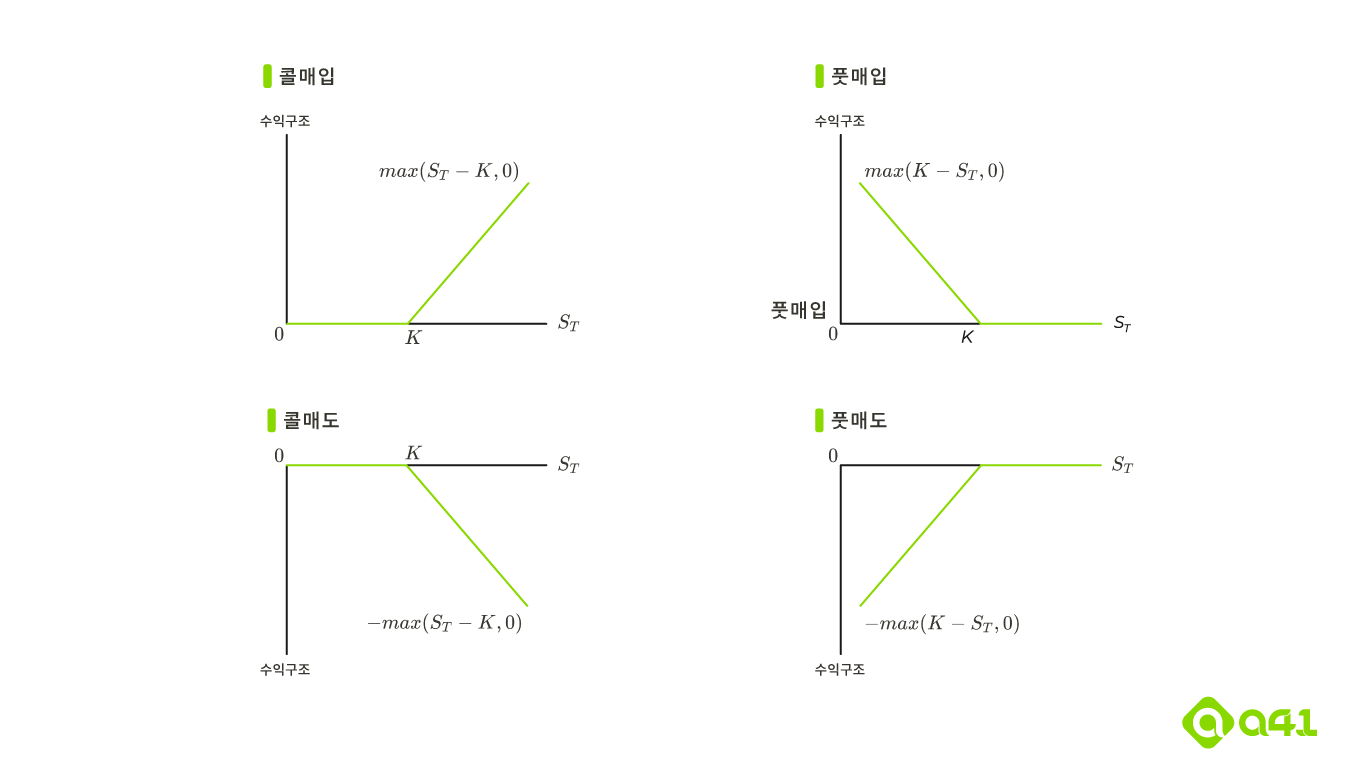
\includegraphics{images/Options_payoff.png}

}

\caption{Options payoff, from A41}

\end{figure}%

옵션의 기초자산은 매우 다양합니다. 여기서는 주식옵션(Stock Options),
ETP옵션, 통화옵션, 지수옵션, 선물옵션(Futures Options)를 위주로 살펴볼
예정입니다.

\section*{10.4\textasciitilde10 Specification of Stock
Options}\label{specification-of-stock-options}
\addcontentsline{toc}{section}{10.4\textasciitilde10 Specification of
Stock Options}

\markright{10.4\textasciitilde10 Specification of Stock Options}

대표적인 예시로, Cboe(Chicago Board Options Exchange)에서 거래되는
주식옵션(American stock option)에 대해서 알아보겠습니다.

\begin{itemize}
\tightlist
\item
  만기구조 : 매월 세번째 금요일 만기 및 연속 4개월물이 상장되는 것이
  기본입니다. 매주 만기가 도래하는 위클리옵션도 존재하며, 만기가 3년
  이상인 LEAPS(Long term equity anticipation securities) 및 시장참여자가
  자유롭게 옵션스펙을 설정하는 비표준물 옵션인 FLEX옵션도 존재합니다.
\item
  행사가격 : 종목별로 \$2.5, \$5, \$10으로 구분됩니다.
\item
  용어 : 특정 옵션에 대해서, 콜 또는 풋 어느 한종류를 지칭할 때 Option
  Class, 전체를 지칭할 때 Options series라고 합니다. 또한, 행사가격과
  현재 기초자산가격에 따라 내재가치가 0보다 큰 옵션을 내가격(ITM, In The
  Money), 내재가치가 0보다 작은 옵션을 외가격(OTM, Out of The Money),
  내재가치가 0인 옵션을 등가격(At The Money)라고 합니다.
\item
  배당 및 증자 : 일반적으로 현금배당은 미결제약정 및 행사가격 등 조정이
  없으나, 주가의 10\%를 초과하는 현금배당은 이사회 의결을 통해
  조정해주곤 합니다. 이외의 증자 및 주식배당의 경우 그 비율만큼 옵션
  미결제약정(또는 기준가격)과 행사가격을 조정하고 있습니다.
\item
  보유한도 : 미결제약정수량 보유한도(Position limit) 및 최대
  행사가능수량(Exercise limit)가 존재하며, 기초주식에 따라 수량 상이.
\item
  거래제도 : 현재는 거의 모든 거래가 전산화되어있으며, 주요 종목에
  양방향 호가를 공급하는 시장조성제도를 운영하고 있어 편리하게 거래가
  가능하며, 반대거래를 통해 언제든지 보유한 포지션을 시장에서 해소할 수
  있음.
\item
  거래비용 : 시장에서 옵션을 거래할 때는, 명시적 비용과 암묵적 비용이
  존재합니다.

  \begin{itemize}
  \tightlist
  \item
    명시적 비용 : 거래세, 거래수수료, 위탁수수료 등
  \item
    암묵적 비용 : 호가스프레드 비용, 시장충격비용 등
  \end{itemize}
\item
  증거금

  \begin{itemize}
  \tightlist
  \item
    매수 : 일반적으로 옵션매수자는 프리미엄(가격)을 거래시점에 전액
    부담하는 것이 일반적이나, 만기가 9개월 이상 남은 장기옵션을 거래할
    때는 프리미엄을 25\%만 부담하고 미수로 거래하는 제도도 존재함
  \item
    매도 : 다른 포지션 없이 옵션 매도만을 가지고 있는 경우, Naked
    option이라고 하며, Cboe는 이 경우 ``옵션매도대금 +
    기초자산가격*20\%'' 수준의 증거금을 징수
  \end{itemize}
\item
  옵션청산회사, OCC : 모든 장내옵션은 OCC를 통해서 청산되며, OCC는
  청산결제 외에도 옵션 매수자의 권리행사가 있는 경우, 매도자에게
  공정하고 합리적으로 배정함으로써 원활히 옵션포지션이 청산될 수 있도록
  관리하고 있음.
\item
  규제기관 : 국내는 금융위에서 모든 규제권한을 가지고 있으나, 미국의
  경우 주식/주가지수/통화옵션은 SEC에서, 선물에 대한 옵션은 CFTC에서
  규제를 관할하고 있음.
\item
  세금 : 옵션거래에 대한 세금은 매우 tricky한 면이 있음. 일반적으로는
  옵션거래에서 발생하는 자본손익(capital gain/loss)에 대해서 세금을
  부과하며, 옵션이 권리행사 또는 기간이 만료되거나/반대거래로 포지션이
  소멸할 때 해당 수익을 인식하고 있음.

  \begin{itemize}
  \tightlist
  \item
    Wash sale rule : 주식을 팔고 30일 이내에 다시 사는 경우는 수익인식을
    안하는데, 유사하게 주식을 팔고 30일 이내에 콜옵션을 매수하는 경우
    수익인식 안함.
  \item
    Constructive Sales : 숏포지션은 해당 포지션을 청산하기 전까지는
    손익인식이 안돼는 점을 방지하기 위해, 즉 공매도나 파생상품
    숏포지션으로 과세를 미루는 것을 막기위해 TaxRelief Act of 1997에서
    (1) 공매도를 하는 경우, (2) 선도/선물계약을 하는 경우, (3) 이와
    유사한 손익구조를 만드는 경우 Constructive Sales로 인식하여 세금을
    부과하도록 규정하였음. 즉, 주식을 매도하지 않고 주식선물/콜옵션을
    매도하거나 풋옵션을 매수하는 경우, 주식을 매도한 것으로 간주하고
    세금을 부과하는 것임.
  \end{itemize}
\item
  주식옵션의 활용

  \begin{itemize}
  \tightlist
  \item
    워런트 : 워런트가 포함된 채권을 BW(Bond with Warrent)라고 하며,
    신주인수권부사채라고도 합니다. 채권에 향후 주식을 특정가격에 매수할
    수 있는 권리인 주식콜옵션이 합쳐진 형태입니다.
  \item
    임직원 스톡옵션 : 임직원 동기부여 및 사기진작을 위해 통상 ATM에
    발행해서 향후 특정시점 이후에 권리행사할 수 있도록 만든
    주식옵션입니다.
  \item
    전환사채 : CB(Convertible bonds)라고 하며, 채권으로 발행되지만 향후
    액면가 대비 정해진 비율에 따라 주식으로 전환할 수 있는 채권입니다.
  \end{itemize}
\item
  장외옵션 : 옵션시장은 장내보다 장외시장이 훨씬 규모가 큰 시장이며,
  일반적인 장내옵션(plain vanilla) 이외에도 다양한 구조로 설계한
  이색옵션(exotic options)이 거래되곤 합니다.
\end{itemize}

\bookmarksetup{startatroot}

\chapter*{Chapter 11}\label{chapter-11}
\addcontentsline{toc}{chapter}{Chapter 11}

\markboth{Chapter 11}{Chapter 11}

Properties of Stock Options

\section*{11.1 Factors Affecting Option
Prices}\label{factors-affecting-option-prices}
\addcontentsline{toc}{section}{11.1 Factors Affecting Option Prices}

\markright{11.1 Factors Affecting Option Prices}

옵션 가격에 영향을 미치는 요소는 크게 6가지가 있으며, 이 변수들과 옵션
가격과의 상관관계는 다음과 같습니다.

\begin{longtable}[]{@{}lcccc@{}}
\toprule\noalign{}
Variable & European Call & European Put & American call & American
put \\
\midrule\noalign{}
\endhead
\bottomrule\noalign{}
\endlastfoot
Current stock price, \(S_0\) & + & - & + & - \\
Strike prkce, \(K\) & - & + & - & + \\
Time to expiration, \(T\) & ? & ? & + & + \\
Volatility, \(\sigma\) & + & + & + & + \\
Risk-free rate, \(r_f\) & + & - & + & - \\
Amount of future dividend, \(d\) & - & + & - & + \\
\end{longtable}

\begin{enumerate}
\def\labelenumi{\arabic{enumi}.}
\tightlist
\item
  주가 및 행사가격 : 만기 pay-off를 고려하면 쉽게 이해할 수 있습니다.
\item
  만기

  \begin{itemize}
  \tightlist
  \item
    미국형 : 언제나 행사할 수 있으므로 만기가 길수록 옵션 가치는 증가
  \item
    유럽형 : 일반적으로 만기가 길수록 옵션 가치가 증가하지만, 중도배당이
    존재하는 경우나 Deep-ITM 풋옵션의 경우에서는 만기가 짧은 옵션이
    유리한 경우도 존재함
  \end{itemize}
\item
  변동성 : 간단히 설명하자면, 옵션 매수자의 경우 이익은 제한이 없고
  손실은 프리미엄으로 제한되어 있으므로 변동성이 클 수록 옵션 기대이익이
  증가하게 되므로 변동성과 옵션가격은 항상 양의 상관관계에 있음
\item
  무위험이자율 : 일반적으로 무위험이자율이 증가하면 주가의 요구수익률이
  증가하게 되고, 더불어 미래 현금흐름의 현재가치가 감소하는 효과가 있음.
  즉, 콜옵션의 가치는 증가하고 풋옵션의 가치는 감소하는 경향이 있음.
\item
  배당 : 배당이 존재하면 배당락으로 주가가 하락함. 콜옵션의 가치는
  감소하고 풋옵션의 가치는 증가함.
\end{enumerate}

\section*{11.2 Assumptions and
Notation}\label{assumptions-and-notation-1}
\addcontentsline{toc}{section}{11.2 Assumptions and Notation}

\markright{11.2 Assumptions and Notation}

이전 챕터와 동일하게 모든 시장참가자는 거래비용이 없고, 동일한 세율을
적용받으며, 무위험이자율로 빌리거나 빌려줄 수 있다는 가정을 사용할 것
입니다.

대문자는 American option을, 소문자는 European option을 의미합니다.

\section*{11.3 Upper and Lower Bounds for Option
Prices}\label{upper-and-lower-bounds-for-option-prices}
\addcontentsline{toc}{section}{11.3 Upper and Lower Bounds for Option
Prices}

\markright{11.3 Upper and Lower Bounds for Option Prices}

\subsection*{Upper bound}\label{upper-bound}
\addcontentsline{toc}{subsection}{Upper bound}

기본적으로, 권리행사를 통해 행사가격을 지불하고 주식을 사거나(콜),
행사가격에 주식을 파는(콜) 옵션의 성질에 따라 콜옵션은 현재 주가보다
비쌀 수 없고, 풋옵션은 행사가격의 현재가치보다 비쌀 수 없습니다.

콜옵션이 현재 주가보다 비싸다면 콜옵션 매도+주식 매수를, 풋옵션이
행사가격의 현재가치보다 비싸다면 풋옵션 매도+무위험이자율에 투자함으로써
간단한 차익거래가 가능하기 때문입니다.

\[C\leq S_0,\;\; c\leq S_0,\;\; P\leq K,\;\; p\leq Ke^{-rT}\]

\subsection*{Lower bound for
Non-dividend}\label{lower-bound-for-non-dividend}
\addcontentsline{toc}{subsection}{Lower bound for Non-dividend}

\subsection*{European}\label{european}
\addcontentsline{toc}{subsection}{European}

두 가지 포트폴리오를 비교해보겠습니다.

\begin{enumerate}
\def\labelenumi{\arabic{enumi}.}
\tightlist
\item
  콜옵션 매수(\(c\)) 및 행사가격의 현재가치(\(Ke^{-rT}\))만큼
  무위험이자율에 투자
\item
  주식을 현재가격(\(S_0\))에 매수
\end{enumerate}

만기시점 \(T\)에 두 포트폴리오의 가치는 다음과 같습니다.

\begin{enumerate}
\def\labelenumi{\arabic{enumi}.}
\tightlist
\item
  \(max(S_T-K,0)+K=max(S_T,K)\)
\item
  \(S_T\)
\end{enumerate}

이에 따라, 포트폴리오 1의 가치는 항상 2보다 커야하므로,
\(c\geq S_0-Ke{-rT}\)가 만족합니다.

마찬가지로,

\begin{enumerate}
\def\labelenumi{\arabic{enumi}.}
\tightlist
\item
  풋옵션 매수(\(p\)) 및 주식을 현재가격(\(S_0\))에 매수
\item
  행사가격의 현재가치(\(Ke^{-rT}\))만큼 무위험이자율에 투자
\end{enumerate}

만기시점 \(T\)에 두 포트폴리오의 가치는 다음과 같습니다.

\begin{enumerate}
\def\labelenumi{\arabic{enumi}.}
\tightlist
\item
  \(max(K-S_T,0)+S_T=max(K,S_T)\)
\item
  \(K\)
\end{enumerate}

이에 따라, \(p\geq Ke{-rT}-S_0\)가 만족합니다.

한편, 옵션의 가치는 항상 0보다 크거나 같아야하므로 배당이 없는 유럽형
옵션의 하한은 다음과 같습니다.

\[c\geq max(S_0-Ke{-rT},0),\;p\geq max(Ke^{-rT}-S_0,0)\]

\subsection*{American}\label{american}
\addcontentsline{toc}{subsection}{American}

먼저, 배당이 없을 때는 콜옵션의 시간가치가 항상 0보다 크거나 같으므로
미국형 콜옵션과 유럽형 콜옵션의 가격이 항상 같습니다.

\begin{tcolorbox}[enhanced jigsaw, toprule=.15mm, breakable, left=2mm, leftrule=.75mm, opacitybacktitle=0.6, coltitle=black, rightrule=.15mm, colback=white, titlerule=0mm, bottomtitle=1mm, colframe=quarto-callout-tip-color-frame, title=\textcolor{quarto-callout-tip-color}{\faLightbulb}\hspace{0.5em}{Tip}, toptitle=1mm, arc=.35mm, colbacktitle=quarto-callout-tip-color!10!white, opacityback=0, bottomrule=.15mm]

배당이 없다면, 조기행사의 가치는 ``0''입니다.

만약, 만기 이전에 내재가치가 높아 미국형 콜옵션을 조기행사하고자 하는
투자자가 있다면, 조기행사 대신에 주식을 공매도하고 공매도대금을
무위험이자율에 투자함으로써 무위험차익을 얻을 수 있습니다.

직관적으로, 주식을 보유함으로써 발생하는 (+) 현금흐름이 없으므로, 미리
주식을 매수함으로써 얻는 이익은 없지만 행사가격만큼의 현금에 대한
기회비용이 발생하기 때문에 조기행사의 가치가 0이됩니다.

반면, 풋옵션의 경우 조기행사함으로써 행사가격만큼 현금이 들어오기 때문에
조기행사할 유인이 발생할 수 있습니다.

\end{tcolorbox}

한편, 미국형 풋옵션은 언제나 권리행사를 할 수 있으므로
\(P\geq max(K-S_0,0)\)의 하한을 갖게 됩니다.

옵션의 종류별로 상한 및 하한을 정리하면 아래와 같습니다.

\[max(S_0-Ke^{-rT})\leq c=C\leq S_0\]

\[max(Ke^{-rT}-S_0)\leq p\leq Ke^{-rT},\;\;max(K-S_0,0)\leq P \leq K\]

\section*{11.4\textasciitilde6 Put-Call Parity}\label{put-call-parity}
\addcontentsline{toc}{section}{11.4\textasciitilde6 Put-Call Parity}

\markright{11.4\textasciitilde6 Put-Call Parity}

옵션 하한을 산출할 때 이용한 포트폴리오를 이용해 콜옵션과 풋옵션의
가격간에 중요한 관계를 유도할 수 있습니다.

콜옵션과 풋옵션의 포트폴리오 1을 주목해봅시다.

\begin{enumerate}
\def\labelenumi{\arabic{enumi}.}
\tightlist
\item
  콜옵션 매수(\(c\)) 및 행사가격의 현재가치(\(Ke^{-rT}\))만큼
  무위험이자율에 투자
\item
  풋옵션 매수(\(p\)) 및 주식을 현재가격(\(S_0\))에 매수
\end{enumerate}

만기시점의 포트폴리오의 가치는 다음과 같습니다.

\begin{enumerate}
\def\labelenumi{\arabic{enumi}.}
\tightlist
\item
  \(max(S_T-K,0)+K=max(S_T,K)\)
\item
  \(max(K-S_T,0)+S_T=max(K,S_T)\)
\end{enumerate}

즉, 두 포트폴리오는 만기 \(T\) 시점에 동일한 Pay-off를 가지고 있는
동일한 포트폴리오입니다.

따라서 두 포트폴리오의 가치는 동일해야하므로, 아래와 같이 Put-Call
parity를 유도할 수 있습니다.

\[c+Ke^{-rT}=p+S_0\]

\begin{tcolorbox}[enhanced jigsaw, toprule=.15mm, breakable, left=2mm, leftrule=.75mm, opacitybacktitle=0.6, coltitle=black, rightrule=.15mm, colback=white, titlerule=0mm, bottomtitle=1mm, colframe=quarto-callout-tip-color-frame, title=\textcolor{quarto-callout-tip-color}{\faLightbulb}\hspace{0.5em}{ATM 옵션의 가격}, toptitle=1mm, arc=.35mm, colbacktitle=quarto-callout-tip-color!10!white, opacityback=0, bottomrule=.15mm]

Put-call parity에서 ATM(\(S_0=K\)) 옵션인 경우,

\[c+S_0e^{-rT}=p+S_0\Rightarrow c-p=S_0(1-e^{-rT})>0\]

즉, ATM에서는 콜옵션의 가치가 풋옵션보다 높은 것을 알 수 있습니다.

\end{tcolorbox}

\subsection*{Parity in American options}\label{sec-AmericanParity}
\addcontentsline{toc}{subsection}{Parity in American options}

풋콜패리티는 유럽형 옵션에서만 성립하므로, 미국형 옵션에서는 이와 유사한
부등식을 유도할 수 있습니다.

먼저, 다음 세가지 포트폴리오를 고려해보겠습니다.

\begin{enumerate}
\def\labelenumi{\arabic{enumi}.}
\tightlist
\item
  콜옵션 매수(\(c\)) 및 행사가격의 현재가치(\(Ke^{-rT}\))만큼
  무위험이자율에 투자
\item
  풋옵션 매수(\(p\)) 및 주식을 현재가격(\(S_0\))에 매수
\item
  미국형 풋옵션 매수(\(P\)) 및 주식을 현재가격(\(S_0\))에 매수
\end{enumerate}

Put-call parity에 따라 1과 2의 가치가 같고, 미국형 옵션의 가치는 유럽형
옵션보다 항상 크거나 같으며, 배당이 없을 때는 미국형 콜옵션과 유럽형
콜옵션의 가격이 같으므로 아래와 같이 정리할 수 있습니다.

\[c+Ke^{-rT}=p+S_0\leq P+S_0\Rightarrow c-P=C-P\leq S_0-Ke^{-rT}\]

다음으로, 두가지 포트폴리오를 고려해보겠습니다.

\begin{enumerate}
\def\labelenumi{\arabic{enumi}.}
\tightlist
\item
  유럽형 콜옵션 매수(\(C\)) 및 행사가격(\(K\))만큼 현금 보유
\item
  미국형 풋옵션 매수(\(P\)) 및 주식을 현재가격(\(S_0\))에 매수
\end{enumerate}

먼저, 조기행사 없이 만기보유하는 경우 두 포트폴리오의 가치는,

\begin{enumerate}
\def\labelenumi{\arabic{enumi}.}
\tightlist
\item
  \(max(S_T-K,0)+Ke^{rT}=max(S_T,K)+K(e^{rT}-1)\)
\item
  \(max(K-S_T,0)+S_T=max(K,S_T)\)
\end{enumerate}

포트폴리오 1에서는 현금에서 무위험이자율만큼 수익이 발생하므로
포트폴리오 2보다 가치가 높게 됩니다.

다음으로, 풋옵션에서 조기행사가 발생하는 경우를 살펴보겠습니다.

조기행사가 \(0<t<T\) 인 t시점에 발생한다면, \(t\)시점에 풋옵션의
포트폴리오 2의 가치는 \(K\)가 되며 만기 \(T\) 시점에는 \(Ke^{r(T-t)}\)가
됩니다.

반면, \(T\) 시점에 포트폴리오 1의 가치는 옵션이 없더라도
\(Ke^{rT}\)이므로, 항상 포트폴리오 1의 가치가 크거나 같게됩니다.

즉, \(C+K=c+K\geq P+S_0\)가 만족하며, 상한 및 하한을 정리하면 아래와
같습니다.

\[S_0-K\leq C-P\leq S_0-Ke^{-rT}\]

\section*{Effect of Dividends}\label{effect-of-dividends}
\addcontentsline{toc}{section}{Effect of Dividends}

\markright{Effect of Dividends}

\subsection*{European}\label{european-1}
\addcontentsline{toc}{subsection}{European}

이제, 배당이 있는 경우를 살펴보겠습니다. 만기시점까지 주식에서 발생하는
배당금의 현재가치를 \(D\)라고 하고, 다음 포트폴리오를 살펴보겠습니다.

\begin{enumerate}
\def\labelenumi{\arabic{enumi}.}
\tightlist
\item
  유럽형 콜옵션 매수(\(c\)) 및 \(D+Ke^{-rT}\)만큼 무위험이자율에 투자
\item
  주식 매수(\(S_0\))
\item
  유럽형 풋옵션 매수(\(p\)) 및 주식 매수(\(S_0\))
\item
  \(D+Ke^{-rT}\)만큼 무위험이자율에 투자
\end{enumerate}

위와 같은 방식으로 만기 \(T\)시점에 각 포트폴리오의 가치를 비교하면,

\begin{enumerate}
\def\labelenumi{\arabic{enumi}.}
\tightlist
\item
  \(max(S_T-K,0)+De^{rT}+K=max(S_T,K)+De^{rT}\)
\item
  \(S_T+De^{rT}\)
\item
  \(max(K-S_T,0)+S_t+De^{rT}=max(K,S_T)+De^{rT}\)
\item
  \(De^{rT}+K\)
\end{enumerate}

각 옵션의 하한 및 풋콜패리티를 정리하면,

\[(1)\geq (2)\Rightarrow c\geq max(S_0-D-Ke^{-rT},0)=max(S_0e^{-dT}-Ke^{-rT})\]

\[(3)\geq (4)\Rightarrow p\geq max(D+Ke^{-rT}-S_0,0)=max(Ke^{-rT}-S_0e^{-dT})\]

\[(3)\equiv(4)\Rightarrow c+D+Ke^{-rT}=p+S_0\Rightarrow c-p=S_0-D-Ke^{-rT}=S_0e^{-dT}-Ke^{-rT}\]

\begin{tcolorbox}[enhanced jigsaw, toprule=.15mm, breakable, left=2mm, leftrule=.75mm, opacitybacktitle=0.6, coltitle=black, rightrule=.15mm, colback=white, titlerule=0mm, bottomtitle=1mm, colframe=quarto-callout-tip-color-frame, title=\textcolor{quarto-callout-tip-color}{\faLightbulb}\hspace{0.5em}{Tip}, toptitle=1mm, arc=.35mm, colbacktitle=quarto-callout-tip-color!10!white, opacityback=0, bottomrule=.15mm]

주식의 배당이 기간 중 연속복리배당수익률 \(d\)로 주어져 있다면,
포트폴리오에서 주식을 매수할 때 \(S_0e^{-dT}\)만큼 매입하고, 배당은
주식에 재투자한다고 가정하면 등식의 마지막 결과를 얻을 수 있습니다.

\end{tcolorbox}

\subsection*{American}\label{american-1}
\addcontentsline{toc}{subsection}{American}

앞서 배당이 없는 경우에서 \(C-P\leq S_0-Ke^{-rT}\)가 성립하는 것을
살펴보았습니다.

변수와 옵션가격 간의 관계에서, 배당은 콜옵션에서 (-), 풋옵션에서 (+)인
것을 확인하였습니다. 나중에 살펴보겠으나, 동일한 배당이 존재한다면 이
둘의 변화는 상쇄될 수 있습니다.

따라서 \(C-P\) 포트폴리오에서 배당이 존재하는 경우, 두 변화분은
상쇄되므로 변동이 없게 되고, 따라서 배당이 존재하는 경우에 대해서도 위의
상한이 성립하게 됩니다.

다음으로, 두가지 포트폴리오를 고려해보겠습니다.

\begin{enumerate}
\def\labelenumi{\arabic{enumi}.}
\tightlist
\item
  유럽형 콜옵션 매수(\(c\)) 및 \(D+K\)를 무위험이자율에 투자
\item
  미국형 풋옵션 매수(\(P\)) 및 주식 매수(\(S_0\))
\end{enumerate}

조기행사가 없다면 만기 \(T\)시점의 가치는 포트폴리오 1이 항상 크거나
같습니다.

\begin{enumerate}
\def\labelenumi{\arabic{enumi}.}
\tightlist
\item
  \(max(S_T-K,0)+(D+K)e^{rT}=max(S_T,K)+De^{rT}+K(e^{rT}-1)\)
\item
  \(max(K-S_T)+S_T+De^{rT}=max(K,S_T)+De^{rT}\)
\end{enumerate}

다음으로, 배당이 발생한 후 조기행사가 \(0<t<T\) 인 t시점에 존재하는
경우, t시점의 포트폴리오 2의 가치는 \(K+De^{rt}\)이며, 만기 \(T\)시점의
가치는 \(Ke^{r(T-t)}+De^{rT}\)입니다.

반면, 포트폴리오 1은 옵션이 없더라도 만기 \(T\) 시점에
\((K+D)e^{rT}\)만큼의 가치가 있으므로 포트폴리오 1의 가치가 항상 크게
됩니다.

따라서, \(C+D+K\geq c+D+K\geq P+S_0\)가 성립하며, 미국형 옵션에서 배당을
반영한 부등식은 아래와 같습니다.

\[S_0e^{-dT}-K=S_0-D-K\leq C-P \leq S_0-Ke^{-rT}\]

\bookmarksetup{startatroot}

\chapter*{Chapter 13}\label{chapter-13}
\addcontentsline{toc}{chapter}{Chapter 13}

\markboth{Chapter 13}{Chapter 13}

이항모형 (Binomial Trees)

옵션의 프라이싱에 대한 가장 유명한 방법 중 하나인 이항모형을 다룹니다.

CRR모형(Cox, Ross, Rubinstein 1979)을 다룰 예정이며, 주가는 랜덤워크를
따르고 차익거래가 발생하지 않는다는 기본적인 가정을 전제합니다. 이는
BSM(Black-Sholes-Merton)모형과 함께 매우 중요한 방법론으로, 이항모형의
step이 많아질 수록 두 모형의 결과값은 동일해집니다. 이러한 성질에
대해서는 chaper15 및 21에서 보다 자세히 다룰 예정입니다.

CRR모형은 (1) 일반적인 no-arbitrage을 기반으로 하고, (2) 미국형 옵션 및
이색옵션을 가치평가하는 데에 직관적이고 유용하며, (3)
위험중립가치평가(Risk-neutral valuation)을 사용한다는 점에서 매우
중요합니다.

\section*{13.1 A one-step binomial model and a no-arbitrate
argument}\label{a-one-step-binomial-model-and-a-no-arbitrate-argument}
\addcontentsline{toc}{section}{13.1 A one-step binomial model and a
no-arbitrate argument}

\markright{13.1 A one-step binomial model and a no-arbitrate argument}

옵션의 만기를 \(T\)라고 할 때, 향후 주가가 T시점까지 오르거나 내리는
단순한 구조로 되어있다고 가정하고, 현재 주가를 \(S_0\), 주가 상승시
\(S_T=S_0\times u\) 및 하락시 \(S_T=S_0\times d\), 행사가격 \(K\)의
유럽형 옵션의 현재가격이 \(f_0\)로 주어져있다고 해보겠습니다.

현재시점에 주식을 \(\Delta\)만큼 매수하고, 1주에 대한 옵션을 매도하는
포트폴리오 \(\Delta S_0-f_0\)를 만든다면, 주가 상승시 포트폴리오의
가치는 \(\Delta S_0u-f_u\) 및 하락시에는 \(\Delta S_0d-f_d\)로
결정됩니다.

여기서, \textbf{해당 포트폴리오를 무위험포트폴리오로 만들어 옵션의
가치를 평가}할 수 있습니다. 해당 포트폴리오가 무위험이라는 의미는 주가
상승 및 하락시의 포트폴리오 가치가 동일하게 되어 변동성이 0이 된다는
것을 말합니다.

즉,
\(\Delta S_0u-f_u=\Delta S_0d-f_d\;\Rightarrow\;\Delta=\frac{f_u-f_d}{S_0u-S_0d}\)인
\(\Delta\)를 도출하여 주식을 매수한다면 해당 포트폴리오는 위험이 0이 될
것 입니다.

\begin{tcolorbox}[enhanced jigsaw, toprule=.15mm, breakable, left=2mm, leftrule=.75mm, opacitybacktitle=0.6, coltitle=black, rightrule=.15mm, colback=white, titlerule=0mm, bottomtitle=1mm, colframe=quarto-callout-tip-color-frame, title=\textcolor{quarto-callout-tip-color}{\faLightbulb}\hspace{0.5em}{13.6 Options Delta}, toptitle=1mm, arc=.35mm, colbacktitle=quarto-callout-tip-color!10!white, opacityback=0, bottomrule=.15mm]

위의 델타는 Opion Greeks 중, 기초자산가격 변동에 따른 옵션가격의
민감도인 델타(\(\Delta\))에 해당합니다.

위의 주식매수+옵션매도 포트폴리오에서 우리는 만기 pay-off를 고정시키는
델타를 산출하였으므로, 이는 현재시점에서 주식가격의 변동분과 옵션가격의
변동분이 상쇄됨을 의미합니다. 즉, 포트폴리오에서 주식의 가격이 1만큼
변할때 이에 대응되는 옵션의 가치변화는 \(\Delta\)에 해당하므로, 이는
기초자산 가격에 대한 옵션가격의 민감도와 같습니다.

한편, 이렇게 옵션을 통해 주식포트폴리오의 가격변동분을 완벽히 상쇄하는
것을 델타헷지(Delta hedging)라 합니다.

\end{tcolorbox}

따라서, 포트폴리오의 주가 상승 및 하락에 따른 가치가
\(\Delta S_0u-f_u\)로 고정되며, no-arbitrage 가정에 따라 \(T\)까지의
수익률은 무위험이자율 \(r_f\)로 정해져야 합니다.

즉, 포트폴리오의 현재가치는 미래 pay-off를 무위험이자율로 할인한
현재가치와 동일해져야 하며,(\(\Delta S_0-f_0=(\Delta S_0u-f_u)e^{-rT}\))
여기에 \(\Delta=\frac{f_u-f_d}{S_0u-S_0d}\)를 대입하여 정리하면, 아래와
같이 옵션의 현재가치를 평가할 수 있습니다.

\(\Rightarrow f_0=\Delta S_0-(\Delta S_0u-f_u)e^{-rT}=\Delta S_0(1-ue^{-rT})+f_ue^{-rT}\)

\(\Rightarrow f_0=\frac{f_u-f_d}{u-d}(1-ue^{-rT})+f_ue^{-rT}=\frac{f_u-f_d-f_uue^{-rT}+f_due^{-rT}+(u-d)f_ue^{-rT}}{u-d}\)

\(\Rightarrow f_0=\frac{f_u(1-de^{-rT})-f_d(1-ue^{-rT})}{u-d}=e^{-rT}\frac{f_u(e^{rT}-d)+f_d(u-e^{rT})}{u-d}\)

\(\Rightarrow f_0=e^{-rT}\frac{f_u(e^{rT}-d)+f_d(1-(e^{rT}-d))}{u-d}=e^{-rT}(f_u\times p+f_d\times(1-p))\;for\;p=\frac{e^{rT}-d}{u-d}\)

\begin{tcolorbox}[enhanced jigsaw, toprule=.15mm, breakable, left=2mm, leftrule=.75mm, opacitybacktitle=0.6, coltitle=black, rightrule=.15mm, colback=white, titlerule=0mm, bottomtitle=1mm, colframe=quarto-callout-important-color-frame, title=\textcolor{quarto-callout-important-color}{\faExclamation}\hspace{0.5em}{Probability of stock price}, toptitle=1mm, arc=.35mm, colbacktitle=quarto-callout-important-color!10!white, opacityback=0, bottomrule=.15mm]

위의 1-step binomial tree는 향후 주식이 상승할때의 가격과 하락할 때의
가격만을 이용하여 전개하고 있습니다.

즉, 주식이 상승할 확률과 하락할 확률은 다루고 있지 않습니다. 따라서,
상승할 확률이 0.5일때와 0.9일때의 옵션 가격은 동일합니다. 이는 매우
역설적으로 보입니다.

이러한 이유는 우리가 옵션을 평가할 때, 주식의 향후 가격을 이용해
상대적으로 평가하였기 때문입니다. 주식의 상승 또는 하락확률은 이미
주식의 상승시 가격과 하락시 가격에 내재되어 있기 때문에, 다시 한번
확률을 고려할 필요가 없어지게 됩니다.

\end{tcolorbox}

\section*{13.2 Risk-Neutral Valuation}\label{risk-neutral-valuation}
\addcontentsline{toc}{section}{13.2 Risk-Neutral Valuation}

\markright{13.2 Risk-Neutral Valuation}

\textbf{위험중립가치평가}란 파생상품을 프라이싱할 때, 모든 투자자가
위험중립적(\emph{risk-neutral})이라고 가정하는 것을 말합니다. 이는 모든
자산의 기대수익률이 무위험이자율과 동일하다는 의미이며, 이러한
투자자들만 존재하는 세상을 \emph{risk-neutrall world}라고 합니다.

위험중립세상은 크게 두가지의 특징이 있습니다.

\begin{enumerate}
\def\labelenumi{(\arabic{enumi})}
\tightlist
\item
  모든 투자자산의 기대수익률은 무위험이자율과 같다.
\item
  따라서, 투자자산의 향후 pay-off를 현재가치로 환산할 때 적용하는
  할인률은 무위험이자율이다.
\end{enumerate}

이제 다시, 현재 주가(\(S_0\))는 \(T\)시점까지 상승(\(S_0u\))하거나
하락(\(S_0d\))하고, 주가가 상승할 확률을 \(p\)라고 가정하면
위험중립세상에서 아래와 같이 표현할 수 있습니다.

\[E(S_T)=S_0e^{rT},\;E(S_T)=p\times S_0u+(1-p)\times S_0d\]

\[\Rightarrow S_0e^{rT}=S_0(p(u-d)+d)\Rightarrow p=\frac{e^{rT}-d}{u-d}\]

즉, 위험중립세상에서 주가의 상승확률은 \(\frac{e^{rT-d}}{u-d}\)와
같으며, 이는 1-step binomial tree에서 전개한
\(f_0=e^{-rT}(f_up+f_d(1-p))\)의 p와 동일합니다. 즉, \textbf{옵션의
현재가치는 위험중립세상에서 주가의 상승/하락 확률에 따른 옵션의 미래
pay-off들의 합의 현재가치와 같다}는 것을 의미하며, 이를 통해
\textbf{위험중립세상에서 평가한 옵션의 가치가 실제 세상에서도 동일하게
적용}된다는 중요한 사실을 알 수 있습니다.

\begin{tcolorbox}[enhanced jigsaw, toprule=.15mm, breakable, left=2mm, leftrule=.75mm, opacitybacktitle=0.6, coltitle=black, rightrule=.15mm, colback=white, titlerule=0mm, bottomtitle=1mm, colframe=quarto-callout-tip-color-frame, title=\textcolor{quarto-callout-tip-color}{\faLightbulb}\hspace{0.5em}{Tip}, toptitle=1mm, arc=.35mm, colbacktitle=quarto-callout-tip-color!10!white, opacityback=0, bottomrule=.15mm]

실제 세상에서 투자자는 위험자산에 투자할 때, 보다 높은 수익률을
기대(\emph{risk-averse})하기 때문에 실제 세상과 위험중립세상은 차이가
있습니다. 그러나, 1-step binomial tree와 위험중립세상에서 주가의
상승확률의 결과를 통해 위험중립세상에서 평가한 파생상품의 가치는 실제
세상에서 동일하게 적용된다는 것을 알 수 있습니다.

한편, 실제 세상(\emph{risk-averse})에서 주가의 기대수익률은
무위험이자율보다 높을 것이므로 실제 세상에서 산출한 상승확률은
위험중립세상보다 클 것 입니다. 다만, 이 확률을 이용하여 옵션을
가치평가하는 경우 미래 pay-off에 적용하는 할인률을 옵션의 기대수익률로
변경해주어야 합니다.

그러나, 주식보다 위험한 자산인 옵션의 할인률을 산출하는 것은 매우
어려우므로, 위험중립세상에서 옵션을 평가하는 것이 실제 세상과 동일하다는
것은 매우 강력한 도구입니다.

\end{tcolorbox}

\section*{13.3 Two-step binomial trees}\label{two-step-binomial-trees}
\addcontentsline{toc}{section}{13.3 Two-step binomial trees}

\markright{13.3 Two-step binomial trees}

\includegraphics[width=3.67in,height=2.27in]{Chapter13_files/figure-latex/mermaid-figure-1.png}

이제, binomial tree를 확장하여 2-step model을 살펴보겠습니다. 주가가
상승하거나 하락하는 것이 2번에 걸쳐서 이루어지고, 각 기점의 시간을
\(\Delta t\)라고 하면, 1-step binomial tree에 따라 다음과 같이 표현할 수
있습니다.

\[f_0=e^{-r\Delta t}(pf_u+(1-p)f_d)\;for\;p=\frac{e^{-r\Delta t}-d}{u-d}\]

또한, 이항모형의 2-step과정은 다음과 같이 표현할 수 있습니다.

\[f_u=e^{-r\Delta t}(pf_{uu}+(1-p)f_{ud})\;and\;f_d=e^{-r\Delta t}(pf_{du}+(1-p)f_{dd})\]

\[\Rightarrow f_0=e^{-r\times 2\Delta t}(p^2f_{uu}+2p(1-p)f_{ud}+(1-p)^2f_{dd})\]

\begin{tcolorbox}[enhanced jigsaw, toprule=.15mm, breakable, left=2mm, leftrule=.75mm, opacitybacktitle=0.6, coltitle=black, rightrule=.15mm, colback=white, titlerule=0mm, bottomtitle=1mm, colframe=quarto-callout-note-color-frame, title=\textcolor{quarto-callout-note-color}{\faInfo}\hspace{0.5em}{13.4 Put options example}, toptitle=1mm, arc=.35mm, colbacktitle=quarto-callout-note-color!10!white, opacityback=0, bottomrule=.15mm]

Binomial tree의 일반화된 식은 콜옵션과 풋옵션에 관계없이 적용할 수
있습니다.

\end{tcolorbox}

\section*{13.5 American Options}\label{american-options}
\addcontentsline{toc}{section}{13.5 American Options}

\markright{13.5 American Options}

Binomial Tree는 미국형옵션을 가치평가할 때 아주 유용한 모형입니다.
유럽형옵션과 동일하게 만기까지 모든 node를 전개한 후, 현재가치로 환산할
때 하나의 node씩 진행하면서 조기행사하였을 때와 비교하면 됩니다.

\[f_u=max[max(K-S_u,0),\;e^{-r\Delta t}(pf_{uu}+(1-p)f_{ud})]\]

\[f_d=max[max(K-S_d,0),\;e^{-r\Delta t}(pf_{du}+(1-p)f_{dd})]\]

\[f_0=max[max(K-S_0,0),\;e^{-r\Delta t}(pf_u+(1-p)f_d)]\]

즉, 위와 같이 만기시점부터 이전 step으로 내려오면서
bootstrapping방식으로 미국형 옵션의 가치를 산출할 수 있습니다.

\section*{\texorpdfstring{13.7 Matching Volatility with \(u\) and
\(d\)}{13.7 Matching Volatility with u and d}}\label{matching-volatility-with-u-and-d}
\addcontentsline{toc}{section}{13.7 Matching Volatility with \(u\) and
\(d\)}

\markright{13.7 Matching Volatility with \(u\) and \(d\)}

앞서 무위험이자율, 주가상승/하락률, 시간의 증분이 주어졌을 때
위험중립확률 \(p=\frac{e^{r\Delta t}-d}{u-d}\)로 결정되는 것을
알아보았습니다.

이제, 주가상승률 및 하락률을 주가변동성을 이용하여 표현해보겠습니다.
주가수익률의 표준편차를 \(\sigma\)라고 할 때, 시간의 증분 \(\Delta t\)
동안의 주가수익률의 표준편차는 \(\sigma\sqrt{\Delta t}\)로 표현할 수
있습니다.

\begin{tcolorbox}[enhanced jigsaw, toprule=.15mm, breakable, left=2mm, leftrule=.75mm, opacitybacktitle=0.6, coltitle=black, rightrule=.15mm, colback=white, titlerule=0mm, bottomtitle=1mm, colframe=quarto-callout-important-color-frame, title=\textcolor{quarto-callout-important-color}{\faExclamation}\hspace{0.5em}{Chapter 15 : 주요 내용}, toptitle=1mm, arc=.35mm, colbacktitle=quarto-callout-important-color!10!white, opacityback=0, bottomrule=.15mm]

주가가 Geometric Brownian Motion을 따른다고
가정하겠습니다.(\(\frac{dS}{S}=\mu dt+\sigma dW_t\))

즉, 주가의 기대수익률이 \(\mu\), 표준편차가 \(\sigma\)이면, 매우 짧은
시간에 대한 주가수익률이
정규분포(\(\frac{\Delta S}{S}\sim N(\mu\Delta t,\sigma^2\Delta t)\))를
따른다고 할 수 있습니다.

이때, 위험중립세상을 가정하면 \(\mu=r\)입니다.

\end{tcolorbox}

앞서 binomial tree의 한단계의 step에서 주가의 변동성을
\(E[X^2]-(E[X])^2\)으로 표현하면 다음과 같이 정리할 수 있습니다.

\[\sigma^2\Delta t=p(u-1)^2+(1-p)(d-1)^2-(e^{r\Delta t}-1)^2\]

\[=p[(u-1)^2-(d-1)^2]+(d-1)^2-e^{2r\Delta t}+2e^{r\Delta t}-1\]

\[=\frac{e^{r\Delta t}-d}{u-d}[(u+d)(u-d)-2(u-d)]+d^2-2d-e^{2r\Delta t}+2e^{r\Delta t}\]

\[=e^{r\Delta t}(u+d)-ud-d^2-2e^{r\Delta t}+2d+d^2-2d-e^{2r\Delta t}+2e^{r\Delta t}\]

\[=e^{r\Delta t}(u+d)-ud-e^{2r\Delta t}..._{(13.13)}\]

여기서, 주가 상승 및 하락에 따른 비율을 동일하고 시간의 증분은 매우 작아
power가 1보다 크면 0으로 수렴한다고 가정하겠습니다. 즉,
\((\Delta t)^k\rightarrow 0\;for\;k>1\;\;\&\;\;S_0ud=S_0du=S_0\Rightarrow ud=1\)

그러면, \(d=\frac{1}{u},u>d\)이며 테일러전개를 통해
\(e^{a\Delta t}=1+a\Delta t,\; e^{a\sqrt{\Delta t}}=1+a\sqrt{\Delta t}+\frac{1}{2}a^2\Delta t\)로
쓸 수 있습니다.

다시 (13.13)에 이를 적용해보겠습니다.

\(e^{r\Delta t}(u+d)-ud-e^{2r\Delta t}=\sigma^2\Delta t\)

\(\Rightarrow e^{r\Delta t}(u+d)-ud=e^{2r\Delta t}+\sigma^2\Delta t\)

\(\Rightarrow e^{r\Delta t}(u+1/u)-1=1+2r\Delta t+\sigma^2\Delta t=e^{2r+\sigma^2\Delta t}\)

\(\Rightarrow u+\frac{1}{u}-e^{-r\Delta t}=e^{(r+\sigma^2)\Delta t}\)

\(\Rightarrow u^2-(e^{(r+\sigma^2)\Delta t}+e^{-r\Delta t})u+1=0\)

\(\Rightarrow u^2-(2+\sigma^2\Delta t)u+1=0\)

\[u=\frac{2+\sigma^2\Delta t\pm\sqrt{4+4\sigma^2\Delta t+\sigma^4 (\Delta t)^2_{\rightarrow 0}-4}}{2}=1\pm\sigma\sqrt{\Delta t}+\frac{1}{2}\sigma^2\Delta t=e^{\pm\sigma\sqrt{\Delta t}}\]

\[\therefore u=e^{\sigma\sqrt{\Delta t}},\;d=e^{-\sigma\sqrt{\Delta t}}\]

위 전개를 통해 얻을 수 있는 \(u,d\)가 CRR모형에서 사용하는 상승 및
하락비율입니다.

\begin{tcolorbox}[enhanced jigsaw, toprule=.15mm, breakable, left=2mm, leftrule=.75mm, opacitybacktitle=0.6, coltitle=black, rightrule=.15mm, colback=white, titlerule=0mm, bottomtitle=1mm, colframe=quarto-callout-important-color-frame, title=\textcolor{quarto-callout-important-color}{\faExclamation}\hspace{0.5em}{In Real-world u\&d}, toptitle=1mm, arc=.35mm, colbacktitle=quarto-callout-important-color!10!white, opacityback=0, bottomrule=.15mm]

위의 \(u,d\)는 위험중립세상에서 산출한 상승 및 하락비율이나, real
world에서도 동일하게 적용할 수 있습니다.

실제 세상에서 주가의 기대수익률을 \(\mu\), 변동성을 \(\sigma\), 주가
상승확률을 \(p^*=\frac{e^{\mu\Delta t}-d}{u-d}\)라고 가정하고
\(E[S_T^2]-(E[S_T])^2=\sigma^2\Delta t\)를 위와 동일하게 전개하면,
동일한 \(u,d\)를 얻을 수 있습니다.

한편, 위험중립세상과 실제 세상에서 변동성은 동일하다고 가정하고 있는데,
이는 걸사노프의 정리(\emph{Girsanov's Theorem})를 이용한 결과입니다.

걸사노프 정리에 따르면, 위험중립세상에서 실제세상으로 전환한다는 것은
측도를 전환(\emph{changing measure})하는 것인데, 측도론에서 실제세상은
P-measure 및 위험중립세상은 Q-measure에 해당합니다.

측도를 전환할 때, 기대성장률은 변화하지만 변동성은 유지되는데, 이것이
위험중립세상에서 실제세상으로 전환할 때 주가의 기대수익률은 변하는 반면
변동성은 유지된다는 것을 의미합니다.

\end{tcolorbox}

\section*{13.8 The Binomial Tree
Formulas}\label{the-binomial-tree-formulas}
\addcontentsline{toc}{section}{13.8 The Binomial Tree Formulas}

\markright{13.8 The Binomial Tree Formulas}

앞선 전개식을 요약하면, 주가의 변동성(\(\sigma\)) 및
무위험이자율(\(r\)), 1-step의 시차(\(\Delta t\))가 주어질 때, 이항모형을
적용한 옵션의 가치를 평가할 수 있습니다.

주가상승률 \(u=e^{\sigma\sqrt{\Delta t}}\), 주가하락률
\(d=\frac{1}{u}\), 주가상승률 \(p=\frac{e^{r\Delta t}-d}{u-d}\),
주가하락률 \(q=1-p\)가 적용됩니다.

지금까지 1-step 또는 2-step의 간단한 이항모형만을 살펴보았으나, 실제
실무에 적용될때는 약 30-step의 이항과정이 진행되며, 이는 옵션의 만기까지
주가흐름에 대한 경우의 수가 \(2^{30}\approx 10^9=10billions\) 이상
된다는 것을 의미합니다. 한편, 이항과정의 step이 많아질수록,
\(\Delta t\)가 매우 작아질수록 이항모형의 결과값은 BSM모형의 결과값으로
수렴하게 됩니다.(Appendix 참조)

\section*{13.11 Binomial Trees in various
Options}\label{binomial-trees-in-various-options}
\addcontentsline{toc}{section}{13.11 Binomial Trees in various Options}

\markright{13.11 Binomial Trees in various Options}

\subsection*{Options on Stocks \& Stock indices with continuous
dividend}\label{options-on-stocks-stock-indices-with-continuous-dividend}
\addcontentsline{toc}{subsection}{Options on Stocks \& Stock indices
with continuous dividend}

주가 및 주가지수의 연속복리 배당수익률이 \(q\)로 주어진 경우입니다.

위험중립세상에서 주가 및 주가지수의 수익률은 무위험이자율과
같아야하므로, 주가의 기대수익률 \(k\)와 배당수익률 \(q\)를 합산한
수익률인 무위험이자율과 같아야합니다.

즉,
\(E[S_{\Delta t}]=S_0e^{r\Delta t}=S_0e^{k\Delta t}e^{q\Delta t},\;\;k=r-q\)입니다.

따라서, 앞선 전개식에서 \(p=\frac{e^{(r-q)\Delta t}-d}{u-d}\)로
변경됩니다.

\subsection*{Options on Currencies}\label{options-on-currencies}
\addcontentsline{toc}{subsection}{Options on Currencies}

이전 장에서 통화선도계약 및 통화스왑의 논리를 생각해봅시다.

현재시점에서 자금을 차입하여 해외통화에 투자한다면, 기대수익률은
\(e^{(r-r_f)\Delta t}\)가 될 것입니다.

즉, \(p=\frac{e^{(r-r_f)\Delta t}-d}{u-d}\)가 적용됩니다.

\subsection*{Options on Futures}\label{options-on-futures}
\addcontentsline{toc}{subsection}{Options on Futures}

선물의 가격 \(F_0=S_0e^{rT}\)로 결정됩니다.

\(F_T=S_T\)이므로, 위험중립세상에서 \(E[F_T]=E[S_T]=S_0e^{rT}\)이며
이항모형에서 이를 적용하면 선물의 기대수익률이 0임을 알 수 있습니다.

\[pF_0u+(1-p)F_0u=E[F_T]=E[S_T]\]

\[\Rightarrow pS_0e^{rT}u+(1-p)S_0e^{rT}d=S_0e^{rT}\]

\[\therefore p=\frac{1-d}{u-d}\]

\bookmarksetup{startatroot}

\chapter*{Chapter 13}\label{chapter-13-1}
\addcontentsline{toc}{chapter}{Chapter 13}

\markboth{Chapter 13}{Chapter 13}

위너과정 및 이토보조정리 (\emph{Wiener Processes and Ito's Lemma})

시간의 흐름에 따라 불확실한 경로로 움직이는 변수를
확률과정(\emph{stochastic process})이라고 합니다. 시간의 흐름이
이산적으로 주어지는지, 연속적으로 주어지는지에 따라서 discrete
variable와 continuous variable로 나눌 수 있으며, 앞서 살펴본 이항모형이
대표적인 discrete variable를 이용한 가치평가라고 할 수 있습니다.

이 장에서는 continuous variable을 가정하고, Wiener processes 등 중요한
확률변수를 살펴볼 것이며, 옵션의 가치평가에 매우 핵심적인 이토의
보조정리도 살펴볼 예정입니다.

\section*{14.1 The Markov Property}\label{the-markov-property}
\addcontentsline{toc}{section}{14.1 The Markov Property}

\markright{14.1 The Markov Property}

마코프 과정(\emph{Markov process})는 특수한 형태의 확률과정으로, 시간의
흐름에 따라 변하는 \textbf{변수의 미래값은 오직 현재 값에만 영향을 받는
확률과정}입니다.

즉, 일주일 단위 주가가 마코브 과정을 따른다면 다음 주의 주가는 오직
현재의 주가에만 영향을 받으며, 일주일 전의 주가는 아무런 영향을 주지
않는다는 의미입니다.

이는 효율적 시장가설(EMH, Efficient Market Hypothesis)의 weak-form을
만족한다는 의미와 유사합니다.

\section*{14.2 Continuous-time Stochastic
Processes}\label{continuous-time-stochastic-processes}
\addcontentsline{toc}{section}{14.2 Continuous-time Stochastic
Processes}

\markright{14.2 Continuous-time Stochastic Processes}

먼저, 마코프 과정을 따르는 확률변수를 생각해보겠습니다. 현재 가격이
\(P_t\)이고, 하루동안의 가격변화는 표준정규분포 \(\phi(0,1)\)를 따른다고
가정하겠습니다. 그럼 2일간의 가격변화의 분포는 어떻게 될까요?

먼저, \textbf{2일간의 가격변화는 각각 하루씩 표준정규분포를 따르는
확률변수로 분할}할 수 있습니다. 각 확률변수는 마코프 과정이므로 하루의
변화가 다음 하루의 변화에 영향을 주지않습니다. 즉, \textbf{각각 하루의
표준정규분포는 서로 독립}입니다.

따라서, 2일간의 가격변화의 평균과 분산은 각각의 평균 및 분산의
합산이므로 \(\phi(0,2)\)를 따르게 될 것입니다. 이를 일반화한다면, 기간
\(T\)동안 주가의 변화가 \(\phi(0,T)\)를 따른다면 매우 작은 시간의 변화
\(\Delta t\)동안의 주가의 변화는 \(\phi(0,\Delta t)\)를 따른다고 할 수
있습니다.

여기서, \textbf{표준편차 \(\sigma\)는 기간의 누적에 \(\sqrt{\;\;}\)의
크기로 변화}한다는 사실에 주목해야합니다.

\subsection*{Wiener Process}\label{wiener-process}
\addcontentsline{toc}{subsection}{Wiener Process}

위너과정은 마코프 과정의 일종으로, 평균변화율(drift rate)이 0이고
변동률(variance rate)이 1인 확률과정입니다. 이는 물리학에서 분자의
음직임을 표현하는데 쓰이기도 하며, 브라운 운동(Brownian motion)이라고도
불립니다.

확률변수 \(z\)가 위너과정을 따른다는 것은, 아래 두 성질을 만족한다는
의미입니다.

Property 1.
\(For\;\Delta t,\;\Delta z=\epsilon\sqrt{\Delta t}\;for\;\epsilon\sim\phi(0,1)\)이다.

Property 2.
\(For\;any\;\Delta t_1\neq\Delta t_2.\;\Delta z_1\;and\;\Delta z_2\;are\;independent.\)

첫번째 성질을 통해 \(\Delta z\)의 평균은 0, 분산은 \(\Delta t\),
표준편차는 \(\sqrt{\Delta t}\)임을 알 수 있고, 두번째 성질을 통해
위너과정이 마코프과정의 한 종류임을 알 수 있습니다.

또한, \(\sqrt{\Delta t}>>\Delta t\;for\;\Delta t\rightarrow0\)이므로
단위시간 \(\Delta t\)가 작아지면 작아질수록 위너과정을 따르는 확률변수
\(\Delta z\)의 변동성(표준편차)은 단위시간 대비 매우 커짐을 알 수
있습니다.

이는 미시세상에서 위너과정을 따르는 확률변수가 매우 복잡하게 움직이는
것을 의미하며, 이를 통해 브라운 운동의 특징 두가지를 도출할 수 있습니다.

\begin{enumerate}
\def\labelenumi{\arabic{enumi}.}
\tightlist
\item
  위너과정을 따르는 확률변수 \(z\)에 대해, 어떠한 구간의 시간을
  관측하더라도 \(z\)의 경로의 길이의 기대값은 무한대로 발산한다.
\item
  특정 값의 \(z\)에 대해, 해당 값을 가지는 횟수는 어떠한 구간의 시간을
  관측하더라도 무한대로 발산한다.
\end{enumerate}

\subsection*{Generalized Wiener
Process}\label{generalized-wiener-process}
\addcontentsline{toc}{subsection}{Generalized Wiener Process}

앞서 평균변화율(drift rate)가 0이고 변동률(variance rate)이 1인
위너과정을 살펴보았습니다.

일반화된 위너과정(GWP)이란, 단위시간에 대해 평균변화율과 변동률이 상수
a, b로 주어진 위너과정을 말합니다.

즉, \(dx=a\,dt+b\,dW\)인 확률과정 \(x\)는 GWP를 따르게 됩니다.

여기서 \(dW\)는 위너과정이므로, 단위시간 \(\Delta t\)가 주어져 있다면
GWP를 따르는 확률변수 \(x\)의 변화량은
\(\Delta x=a\,\Delta t+b\,\epsilon\sqrt{\Delta t}\)으로 표현할 수
있습니다.

따라서, \(\Delta x\)의 평균은 \(a\,\Delta t\), 분산은
\(b^2\,\Delta t\)이며 변동성(표준편차)은 \(b\,\sqrt{\Delta t}\)가 되며,
단위시간이 충분히 작다면 \(\Delta x\sim\phi(a\Delta t,b^2\Delta t)\)로
근사할 수 있습니다.

\begin{tcolorbox}[enhanced jigsaw, toprule=.15mm, breakable, left=2mm, leftrule=.75mm, opacitybacktitle=0.6, coltitle=black, rightrule=.15mm, colback=white, titlerule=0mm, bottomtitle=1mm, colframe=quarto-callout-note-color-frame, title=\textcolor{quarto-callout-note-color}{\faInfo}\hspace{0.5em}{기간 T에 대한 GWP의 분포}, toptitle=1mm, arc=.35mm, colbacktitle=quarto-callout-note-color!10!white, opacityback=0, bottomrule=.15mm]

\(x\)가 GWP를 따른다고 가정하고, 기간 \(T\)년과 충분히 작은 단위시간
\(\Delta t,\;\sum_{k=1}^N\Delta t=N\Delta t=T\)가 주어져있다고
가정하겠습니다.

각각의 \(\Delta x_i=a\Delta t+b\epsilon_i\sqrt{\Delta t}\)도 역시 GWP를
따르게 되며, 모두 독립입니다.

그러면, 확률변수 \(x\)의 기간중 누적변화 \(x_T-x_0=\sum\Delta x_i\)는
아래와 같이 전개할 수 있습니다.

\[\sum\Delta x_i=\sum a\Delta t+\sum b\epsilon_i\sqrt{\Delta t}=a\,T+b\sqrt{\Delta t}\sum \epsilon_i\]

각각의 \(\epsilon_i\sim\phi(0,1)\)은 독립이므로
\(\sum \epsilon_i\sim\phi(0,N)\)입니다. 따라서,

\[x_t-x_0\sim\phi(aT,b^2\Delta t\,N)=\phi(aT,b^2T)\]

\end{tcolorbox}

위너과정, \(a\,dt\) 및 GWP의 경로를 도식화하면 아래와 같습니다.

\begin{figure}[H]

{\centering 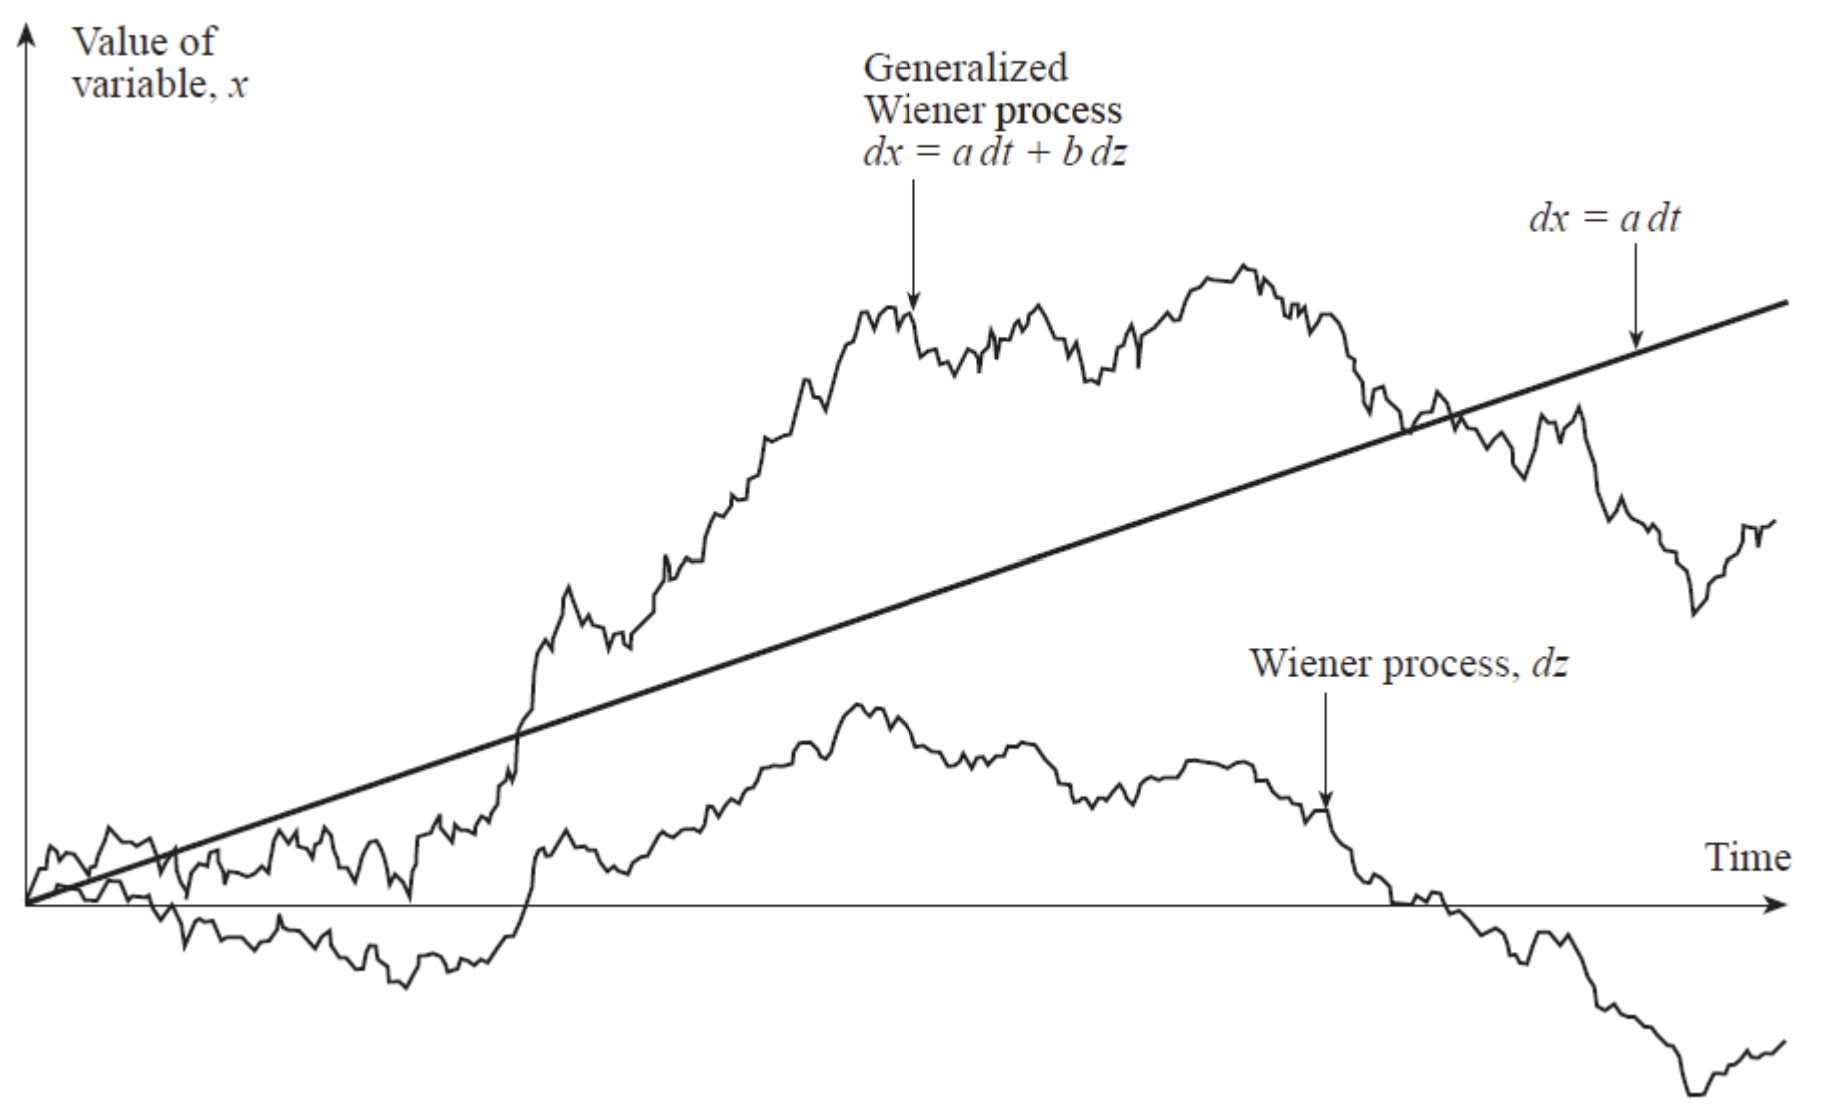
\includegraphics{images/chapter14-1.png}

}

\caption{Path of Stochastic processes :
\(dW,\;\;a\,dt,\;\;a\,dt+b\,dW\)}

\end{figure}%

\begin{tcolorbox}[enhanced jigsaw, colback=white, toprule=.15mm, breakable, left=2mm, leftrule=.75mm, colframe=quarto-callout-color-frame, opacityback=0, arc=.35mm, rightrule=.15mm, bottomrule=.15mm]

\vspace{-3mm}\textbf{14.8 Fractional Brownian Motion}\vspace{3mm}

지금까지 살펴본 브라운운동(위너과정, GWP)은 마코프 과정의 특수한
형태로서 소개하였습니다.

즉, 확률변수 \(X\)가 GWP를 따른다면 각 \(\Delta t\)에 대해
\(\Delta X\)는 독립적으로 결정됩니다. 이는 \(t>s>0\)로 시간이 주어질 때
\(X(t)-X(s),\;X(s)\)가 독립이라는 의미이므로, 다음과 같이 정리할 수
있습니다.
\[Var[X(t)-X(s)]=E[(X(t)-X(s))^2]-E[X(t)-X(s)]^2=\sigma^2(t-s)\]

\(E[X(s)X(t)]=E[X(s)^2]+E[X(s)(X(t)-X(s))]=s\sigma^2\)\$

그러나, \textbf{실제 현실에서는 주가의 흐름이 마코프 과정을 따르지 않는
경우}가 발생합니다. 즉, 주가의 흐름이 과거 주가에 영향을 받는
\textbf{자기상관성}이 관측되고는 합니다.

이러한 경우를 모델링(e.g.~rough volatility models)하기 위해 등장한
개념이 Fractional Brownian Motion입니다.

FBM은 브라운 운동을 일반화한 개념으로, 시간이 \(t>s>0\)로 주어졌을 때,
자기상관성의 척도로 \(H\)(Hurst exponent)가 주어지며, 다음과 같이
정의됩니다.

\[E[(X(t)-X(s))^2]=\sigma^2(t-s)^{2H},\;E[X(s)X(t)]=\frac{\sigma^2}{2}(t^{2H}+s^{2H}-(t-s)^{2H})\]

\(H>0.5\)일때 양의 자기상관성, \(H<0.5\)일때 음의 자기상관성,
\(H=0.5\)일 때 마코프 과정(랜덤워크)을 띄게 되는 브라운 운동입니다.

\end{tcolorbox}

\subsection*{Ito's Process}\label{itos-process}
\addcontentsline{toc}{subsection}{Ito's Process}

일반화된 위너과정에서 평균변화율과 변동률이 상수로 주어졌다면,
이토과정에서는 평균변화율과 변동률이 시간과 확률변수에 대한 함수
\(a(x,t),\;b(x,t)\)로 주어지게 됩니다. 즉,

\[dx=a(x,t)\,dt+b(x,t)\,dW,\;\;\Delta x=a(x,t)\Delta t+b(x,t)\epsilon\sqrt{\Delta t}\]

이를 통해 이토과정도 마코프과정의 한 종류임을 알 수 있습니다.

\section*{14.3 The Process for a Stock
Price}\label{the-process-for-a-stock-price}
\addcontentsline{toc}{section}{14.3 The Process for a Stock Price}

\markright{14.3 The Process for a Stock Price}

이제, 배당이 없는 주식에 대해 확률과정을 모델링해보겠습니다.

먼저 \textbf{주가가 일반화된 위너과정(GWP)를 따른다고 가정}한다면,
평균변화율과 변동률이 상수인 확률과정 \(dS=a\,dt+b\,dW\)를 생각할 수
있습니다.

그러나, 이는 \textbf{주가의 변화분이 상수로 고정}되어있다는 의미인데
현실과 부합하지 않는 부분이 존재합니다. \textbf{실제 주식투자자}는 현재
주가가 높고 낮음에 관계없이 \textbf{투자자금 대비 기대수익률을
고려}하는데, 그렇다면 동일한 기대수익률 하에 \textbf{주가의 변화분이
현재 주가에 따라 달라지기 때문}입니다.

따라서, 주가 대신에 주가수익률이 GWP를 따른다고 가정하는 것이 보다
현실에 부합하게 되며 평균변화율이 \(\mu\), 변동률이 \(\sigma\)로
주어져있다면 주가수익률은 다음과 같은 이토과정을 따른다고 할 수
있습니다. 이러한 \textbf{주식의 확률과정을 기하학적 브라운 운동(GBM,
Geometric Brownian Motion)}이라고도 합니다.

\[dS=\mu\,S\,dt+\sigma\,S\,dW \Rightarrow\]

\[\frac{dS}{S}=\mu\,dt+\sigma\,dW,\;\;\frac{\Delta S}{S}=\mu\Delta t+\sigma\epsilon\sqrt{\Delta t}\]

단위시간 \(\Delta t\)에 대해 평균은 \(\mu\Delta t\), 분산은
\(\sigma^2\Delta t\)이며 표준편차는 \(\sigma\sqrt{\Delta t}\)이고,
단위시간이 충분히 작다면
\(\frac{\Delta S}{S}\sim\phi(\mu\Delta t,\sigma^2\Delta t)\)입니다.

즉, \textbf{\(\mu\)와 \sigma는 각각 단위시간에 대한 주가의 기대수익률과
표준편차를 연율로 환산}한 것입니다.

\begin{tcolorbox}[enhanced jigsaw, toprule=.15mm, breakable, left=2mm, leftrule=.75mm, opacitybacktitle=0.6, coltitle=black, rightrule=.15mm, colback=white, titlerule=0mm, bottomtitle=1mm, colframe=quarto-callout-warning-color-frame, title=\textcolor{quarto-callout-warning-color}{\faExclamationTriangle}\hspace{0.5em}{Warning}, toptitle=1mm, arc=.35mm, colbacktitle=quarto-callout-warning-color!10!white, opacityback=0, bottomrule=.15mm]

단위시간에 대한 주가수익률은 정규분포로 근사할 수 있으나, 기간 \(T\)에
대한 주가 \(S_T-S_0\)는 평균변화율(\(\mu\,S_t\))이 상수로 주어져있지
않기 때문에 14.2의 GWP와 동일한 방법으로 전개할 수 없습니다.

대신에, 주가의 연환산 기대수익률 및 표준편차가 주어져있다면
\(\frac{\Delta S}{S}\sim\phi(\mu\Delta t,\sigma^2\Delta t)\)를 이용한
몬테카를로 시뮬레이션(Monte Carlo Simultation)을 통해 주가 \(S_T\)를
모델링할 수 있습니다.

\end{tcolorbox}

\section*{14.6 Ito's Lemma}\label{itos-lemma}
\addcontentsline{toc}{section}{14.6 Ito's Lemma}

\markright{14.6 Ito's Lemma}

앞선 장에서 우리는 \textbf{파생상품의 가격결정}이 기초자산과의
관계로부터 시작하여 \textbf{기초자산의 현재가격을 통해 결정}된다는 것을
살펴보았습니다. 즉, \textbf{파생상품의 가격은 기초자산의 가격의
함수}입니다.

여기에 확률과정을 적용하면, \textbf{파생상품의 가격은 확률변수인
기초자산의 가격과 시간에 대한 함수}형태로 표현할 수 있다는 것입니다.
그렇다면 \textbf{확률변수를 이용한 함수는 어떤 방식으로 움직이며, 어떠한
확률과정}을 따르게 되는걸까요? 여기서 \textbf{이토의
보조정리(\emph{Ito's Lemma})}라고 불리는 아주 중요한 개념이 등장합니다.

이토의 보조정리란, 이토과정을 따르는 확률변수 \(dx=a(x,t)dt+b(x,t)dW\)와
확률변수 및 시간에 대한 함수 \(G=f(x,t)\)가 주어져있을 때, \(G\)가
다음과 같은 확률과정을 따르게 된다는 정리입니다.

\[dG=(\frac{\partial G}{\partial x}a+\frac{\partial G}{\partial t}+\frac{1}{2}\frac{\partial^2 G}{\partial x^2}b^2)dt+\frac{\partial G}{\partial x}b\,dW\]

즉, 평균변화율이
\(\frac{\partial G}{\partial x}a+\frac{\partial G}{\partial t}+\frac{1}{2}\frac{\partial^2 G}{\partial x^2}b^2\)이며
변동률이 \(\frac{\partial G}{\partial x}b\)인 \textbf{이토과정}을
따른다는 의미입니다.

이제, 파생상품의 가격 \(G=f(S,t)\)와 주가의 확률과정
\(dS=\mu\,S\,dt+\sigma\,S\,dW\)에 이토의 보조정리를 적용하겠습니다.

\[dG=(\frac{\partial G}{\partial S}\mu\,S+\frac{\partial G}{\partial t}+\frac{1}{2}\frac{\partial^2 G}{\partial S^2}\sigma^2\,S^2)dt+\frac{\partial G}{\partial S}\sigma\,S\,dW\]

즉, \textbf{파생상품의 가격 역시 기초자산과 유사한 이토과정}을 따르게
되며, \textbf{동일한 위너과정 \(dW\)에 의해 그 경로가 결정}됩니다. 이
개념은 다음 장의 BSM(Black Sholes Merton) 모형의 결과를 도출할 때
핵심개념으로 이용됩니다.

\section*{14.7 Application of Ito's
Lemma}\label{application-of-itos-lemma}
\addcontentsline{toc}{section}{14.7 Application of Ito's Lemma}

\markright{14.7 Application of Ito's Lemma}

\subsection*{Forward Contract}\label{forward-contract}
\addcontentsline{toc}{subsection}{Forward Contract}

\(t\)시점의 선도가격은 \(F_0=S_0e^{r(T-t)}\)이므로, 무위험이자율이
주어져있다면 이토의 보조정리를 적용할 수 있습니다.

\[dF=(\frac{\partial F}{\partial S}\mu\,S+\frac{\partial F}{\partial t}+\frac{1}{2}\frac{\partial^2 F}{\partial S^2}\sigma^2\,S^2)dt+\frac{\partial F}{\partial S}\sigma\,S\,dW\]

\[=(e^{r(T-t)}\mu\,S-rSe^{r(T-t)})dt+e^{r(T-t)}\sigma\,S\,dW\]

\[\therefore\;dF=(\mu-r)\,F\,dt+\sigma\,F\,dW\]

\subsection*{The Lognormal property}\label{the-lognormal-property}
\addcontentsline{toc}{subsection}{The Lognormal property}

\(G=ln\,S\)라고 하면,
\(\frac{dG}{dS}=\frac{1}{S},\;\frac{dG}{dt}=0,\;\frac{d^2G}{dS^2}=-\frac{1}{S^2}\)

\[dG=(\frac{\partial G}{\partial S}\mu\,S+\frac{\partial G}{\partial t}+\frac{1}{2}\frac{\partial^2 G}{\partial S^2}\sigma^2\,S^2)dt+\frac{\partial G}{\partial S}\sigma\,S\,dW\]

\[=(\frac{1}{S}\mu\,S-\frac{1}{2}\frac{1}{S^2}\sigma^2S^2)dt+\frac{1}{S}\sigma\,S\,dW\]

\[\therefore\;dG=(\mu-\frac{1}{2}\sigma^2)dt+\sigma\,dW\]

이토의 보조정리에 따라, 이토과정을 따르는 주가에 자연로그를 취하면 GWP를
따르게 됩니다. 이제, 14.2의 전개식을 적용하면 기간 \(T\)에 대한 주가의
로그수익률이 정규분포를 따르게 됨을 유도할 수 있습니다.

\[ln\,S_T-ln\,S_0=ln\frac{S_t}{S_0}\sim\phi((\mu-\frac{1}{2}\sigma^2)T,\sigma^2\,T)\]

\bookmarksetup{startatroot}

\chapter*{선물옵션
HW(\textasciitilde midterm)}\label{uxc120uxbb3cuxc635uxc158-hwmidterm}
\addcontentsline{toc}{chapter}{선물옵션 HW(\textasciitilde midterm)}

\markboth{선물옵션 HW(\textasciitilde midterm)}{선물옵션
HW(\textasciitilde midterm)}

\section*{Chapter3}\label{chapter3}
\addcontentsline{toc}{section}{Chapter3}

\markright{Chapter3}

\subsection*{\texorpdfstring{\textbf{Problem 3.4} (Hedging with
Futures)}{Problem 3.4 (Hedging with Futures)}}\label{problem-3.4-hedging-with-futures}
\addcontentsline{toc}{subsection}{\textbf{Problem 3.4} (Hedging with
Futures)}

A company has a \textbf{\$20 million portfolio} with \textbf{a beta of
1.2}. It would like to use futures contracts on a stock index to hedge
its risk. The index \textbf{futures price currently stading at 1080},
and each contract is for delivery of \textbf{\$250 times} the index.

\begin{enumerate}
\def\labelenumi{(\arabic{enumi})}
\item
  what is the hedge that minimizes risk?
\item
  what should the company do if it wants to reduce the beta of the
  portfolio to 0.6?
\end{enumerate}

\textbf{Solving}

먼저, 선물 1계약의 가치는 \(1,080\times 250USD=270,000USD\)입니다.

리스크 최소화를 위한 최적 헷지비율은
\(\hat{h}^*=\beta\times\frac{V_{portfolio}}{V_{futures contract}}\)이므로,

\begin{enumerate}
\def\labelenumi{(\arabic{enumi})}
\item
  리스크 최소화를 위해서는
  \(\hat{h}^*=1.2\times\frac{20,000,000}{270,000}=88.89\approx 89계약\)을
  매도하면 된다.
\item
  베타를 0.6으로 줄이기 위해서는 포트폴리오 베타를 0.6만큼 헷지하면
  된다. \(h=0.6\times\frac{20,000,000}{270,000}=44.44\approx 44계약\)을
  매도하면 된다.
\end{enumerate}

\subsection*{\texorpdfstring{\textbf{Problem 3.24}
(CAPM)}{Problem 3.24 (CAPM)}}\label{problem-3.24-capm}
\addcontentsline{toc}{subsection}{\textbf{Problem 3.24} (CAPM)}

A portfolio manager has maintained an \textbf{actively managed portfolio
with a beta of 0.2}. During the last year, the \textbf{risk-free rate
was 5\%} and \textbf{equities performed very badly providing a return of
-30\%}. The portfolio manager produced \textbf{a return of -10\%} and
claims that in the circumstances \textbf{it was a good performance}.
Discuss this claim.

\textbf{Solving}

CAPM에 근거하여 수익률을 산출할 때, \textbf{매니저의 주장은 옳지 않다.}

먼저, CAPM에 근거한 포트폴리오 수익률은
\(R_{portfolio}=r_f+\beta(r_{market}-r_f)\)이며, 여기에 따르면 베타가
0.2인 주식포트폴리오의 기대수익률은 무위험자산 : 시장 = 8:2로 투자한
시장포트폴리오의 수익률인 \(5\% + 0.2(-30\%-5\%)=-2\%\)이다.

즉, 매니저가 good performance라는 의미는 -2\%보다 높은 수익률을 달성해서
시장포트폴리오를 out-perform한다는 의미인데, 이를 8\%나 하회하는 -10\%의
성적을 거두었으니 좋은 성과를 냈다고 볼 수 없다.

\begin{tcolorbox}[enhanced jigsaw, toprule=.15mm, breakable, left=2mm, leftrule=.75mm, opacitybacktitle=0.6, coltitle=black, rightrule=.15mm, colback=white, titlerule=0mm, bottomtitle=1mm, colframe=quarto-callout-warning-color-frame, title=\textcolor{quarto-callout-warning-color}{\faExclamationTriangle}\hspace{0.5em}{잘못푼 예시}, toptitle=1mm, arc=.35mm, colbacktitle=quarto-callout-warning-color!10!white, opacityback=0, bottomrule=.15mm]

시장 전체의 수익률이 -30\%일 때, 베타가 0.2인 주식포트폴리오가 시장을
beat하는 수익률은 \(0.2\times -30\% =-6\%\)이다. 포트폴리오가 good
performance라는 것은 보통 시장을 out-perform한 경우를 의미하는데,
수익률이 -6\%를 하회하는 -10\%이므로 좋은 성과를 냈다고 보기 어렵다.

\end{tcolorbox}

\subsection*{\texorpdfstring{\textbf{Problem 3.25} (Changing
Beta)}{Problem 3.25 (Changing Beta)}}\label{problem-3.25-changing-beta}
\addcontentsline{toc}{subsection}{\textbf{Problem 3.25} (Changing Beta)}

It is July 16. A company has \textbf{a portfolio of stocks worth
\$100million}. The \textbf{beta of the portfolio is 1.2}. The company
would like to use the December futures contract on a stock index to
\textbf{change beta of the portfolio to 0.5} during the period July 16
to November 16. The \textbf{index is currently 2,000} and each contract
is on \textbf{\$250 times} the index.

\begin{enumerate}
\def\labelenumi{(\arabic{enumi})}
\item
  What position should the company take?
\item
  Suppose that the company changes its mind and decides to increase the
  beta of the portfolio from 1.2 to 1.5. What position in futures
  contracts should it take?
\end{enumerate}

\textbf{Solving}

\emph{Problem 3.4}와 동일한 방식이다. 먼저, 선물 1계약의 가치는
\(2,000\times 250USD=500,000USD\)이며,

\begin{enumerate}
\def\labelenumi{(\arabic{enumi})}
\item
  포트폴리오 베타를 0.5로 줄이려면 베타를 0.7만큼 헷지하면 된다.
  \(h=0.7\times\frac{100,000,000}{500,000}=140계약\)을 매도 하면 된다.
\item
  포트폴리오 베타를 1.5로 늘리려면 베타를 -0.3만큼 헷지하면 된다. 즉,
  매도헷지 대신 선물매수를 통해 베타를 0.3만큼 늘리면 된다.
  \(h=-0.3\times\frac{100,000,000}{500,000}=-60계약 매도=60계약 매수\)하면
  된다.
\end{enumerate}

\section*{Chapter4}\label{chapter4}
\addcontentsline{toc}{section}{Chapter4}

\markright{Chapter4}

\subsection*{\texorpdfstring{\textbf{Problem
4.2}}{Problem 4.2}}\label{problem-4.2}
\addcontentsline{toc}{subsection}{\textbf{Problem 4.2}}

\begin{figure}[H]

{\centering 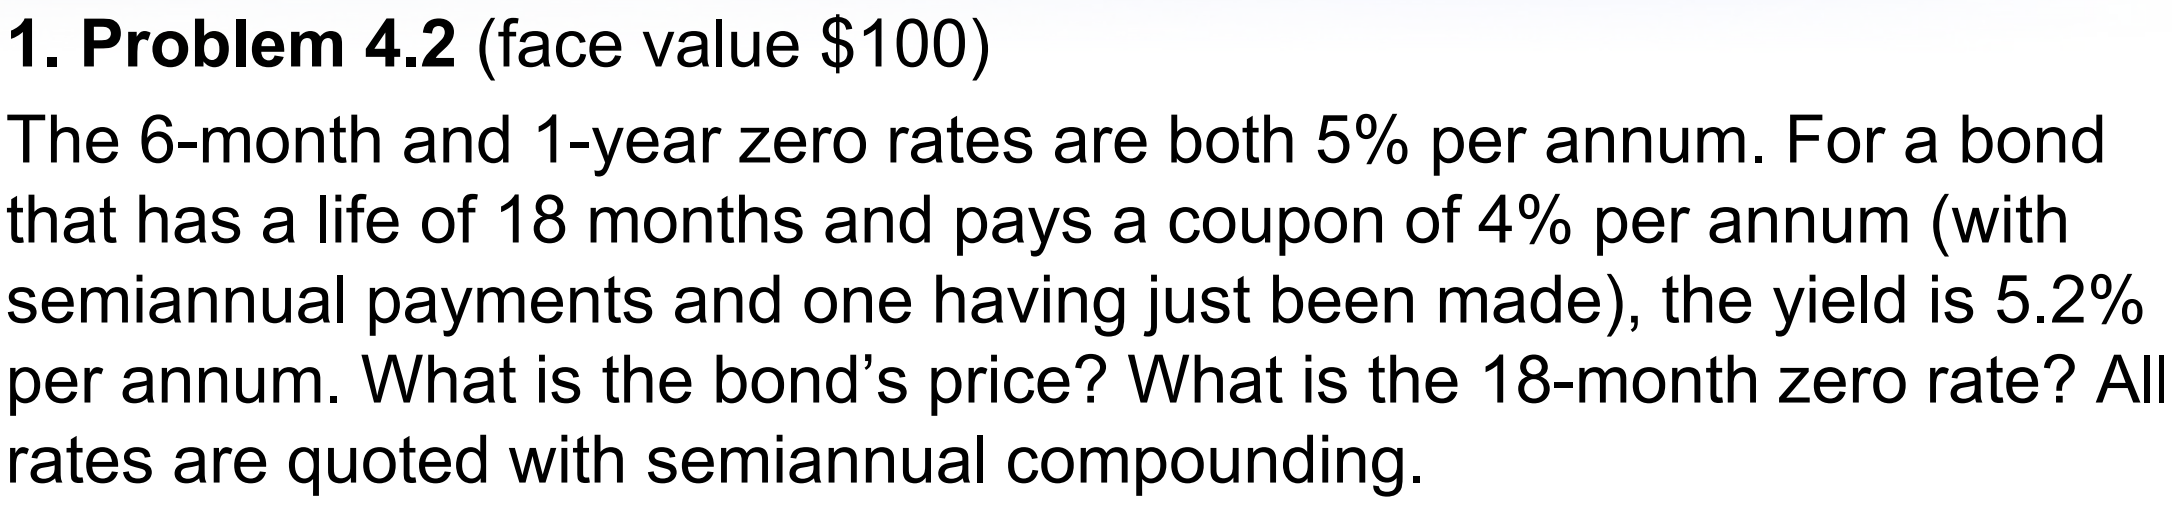
\includegraphics{images/선물옵션_4-2.png}

}

\caption{Chapter4-2}

\end{figure}%

\textbf{Solving}

\[Price=\frac{2}{(1+5.2\%/2)^{1}}+\frac{2}{(1+5.2\%/2)^{2}}+\frac{102}{(1+5.2\%/2)^{3}}=98.29\]

\[\frac{2}{(1+5\%/2)^{1}}+\frac{2}{(1+5\%/2)^{2}}+\frac{102}{(1+z_{1.5}/2)^{3}},\;z_{1.5}=5.204\%\]

\subsection*{\texorpdfstring{\textbf{Problem
4.14}}{Problem 4.14}}\label{problem-4.14}
\addcontentsline{toc}{subsection}{\textbf{Problem 4.14}}

\begin{figure}[H]

{\centering 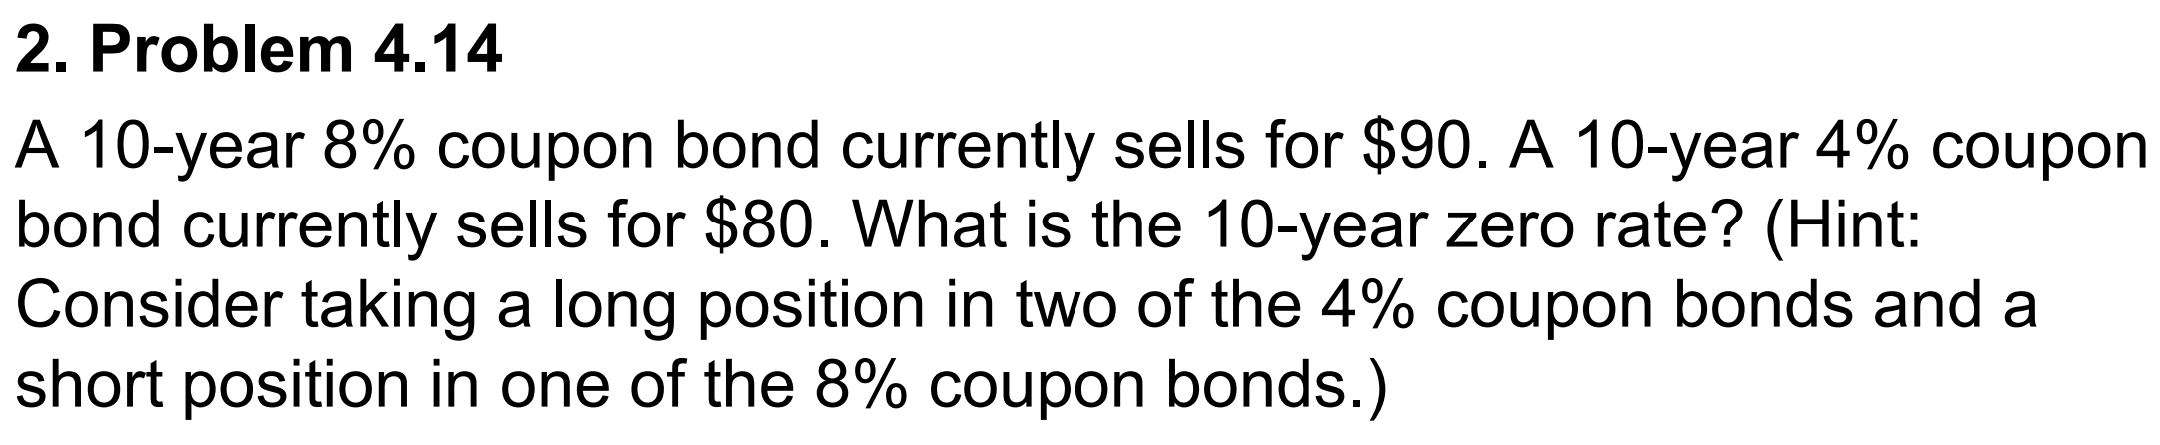
\includegraphics{images/선물옵션_4-14.png}

}

\caption{Chapter4-14}

\end{figure}%

\textbf{Solving}

4\% 쿠폰 채권을 액면 \$200만큼 매수한다면, 액면 \$100의 8\% 쿠폰 채권과
액면 \$100의 10년 무이표채 채권을 매수한 것과 동일한 현금흐름이
발생한다.

이 경우, 10년 무이표채 채권의 가격은 \$160-\$90=\$70이며 10-year zero
rate는 다음과 같다.
\[70=\frac{100}{(1+z_{10})^{10}},\;z_{10}\approx 3.63\%\]

\subsection*{\texorpdfstring{\textbf{Problem
4.29}}{Problem 4.29}}\label{problem-4.29}
\addcontentsline{toc}{subsection}{\textbf{Problem 4.29}}

\begin{figure}[H]

{\centering 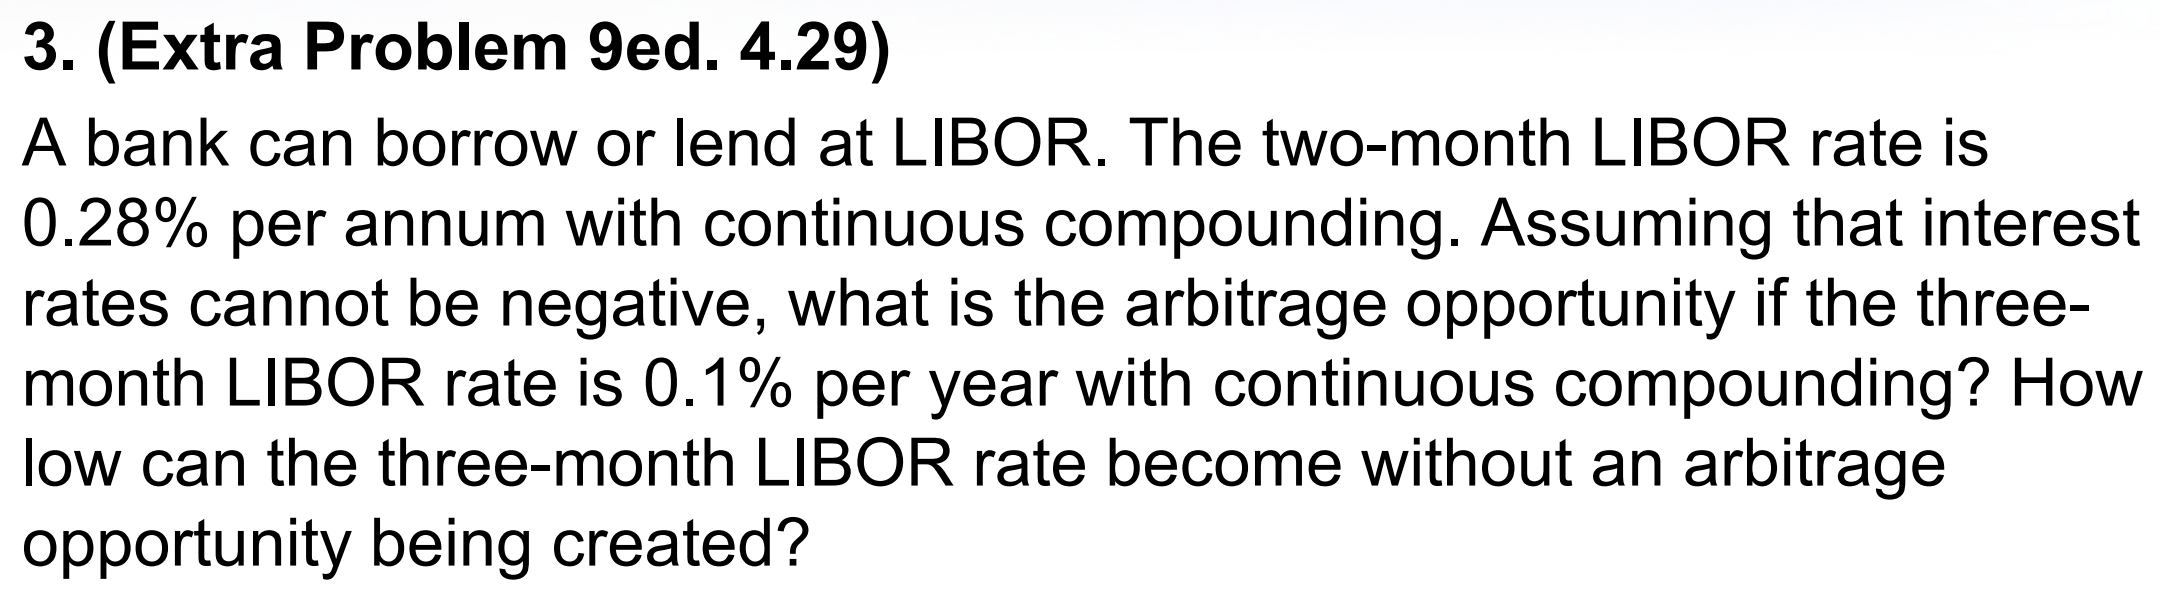
\includegraphics{images/선물옵션_4-29.png}

}

\caption{Chapter4-29, 9ed.}

\end{figure}%

\textbf{Solving}

먼저, 2개월 후 1개월간 Libor Foward rate는 다음과 같다.

\[F_{2m,1m}=\frac{\frac{3}{12}0.1\%-\frac{2}{12}0.28\%}{\frac{1}{12}}=0.3\%-0.56\%=-0.26\%\]

그러나, 이자율은 음수가 될 수 없으므로 선도이자율은 0\%이다. 빌려주는
사람 입장에서, 안빌려주고 현금을 보유하면 이자율은 0\%이므로 이는
자연스러운 현상이다.

이 때, Libor금리로 3개월간 자금을 빌리고 2개월간 Libor로 빌려준 다음
3개월까지는 현금을 보유(또는 0\%에 빌려줌)한다면 무위험 차익을 얻을 수
있다.

차익거래가 발생하지 않으려면, 선도이자율의 균형가격이 0\%까지 상승해야
한다.

\[F_{2m,1m}=0\%=\frac{\frac{3}{12}Libor_{3m}-\frac{2}{12}0.28\%}{\frac{1}{12}}\Rightarrow Libor_{3m}\approx 0.1867\%\]

그러기 위해서는 약 0.1867\%까지 3개월 Libor가 상승해야 한다.

\subsection*{\texorpdfstring{\textbf{Problem
4.39}}{Problem 4.39}}\label{problem-4.39}
\addcontentsline{toc}{subsection}{\textbf{Problem 4.39}}

\begin{figure}[H]

{\centering 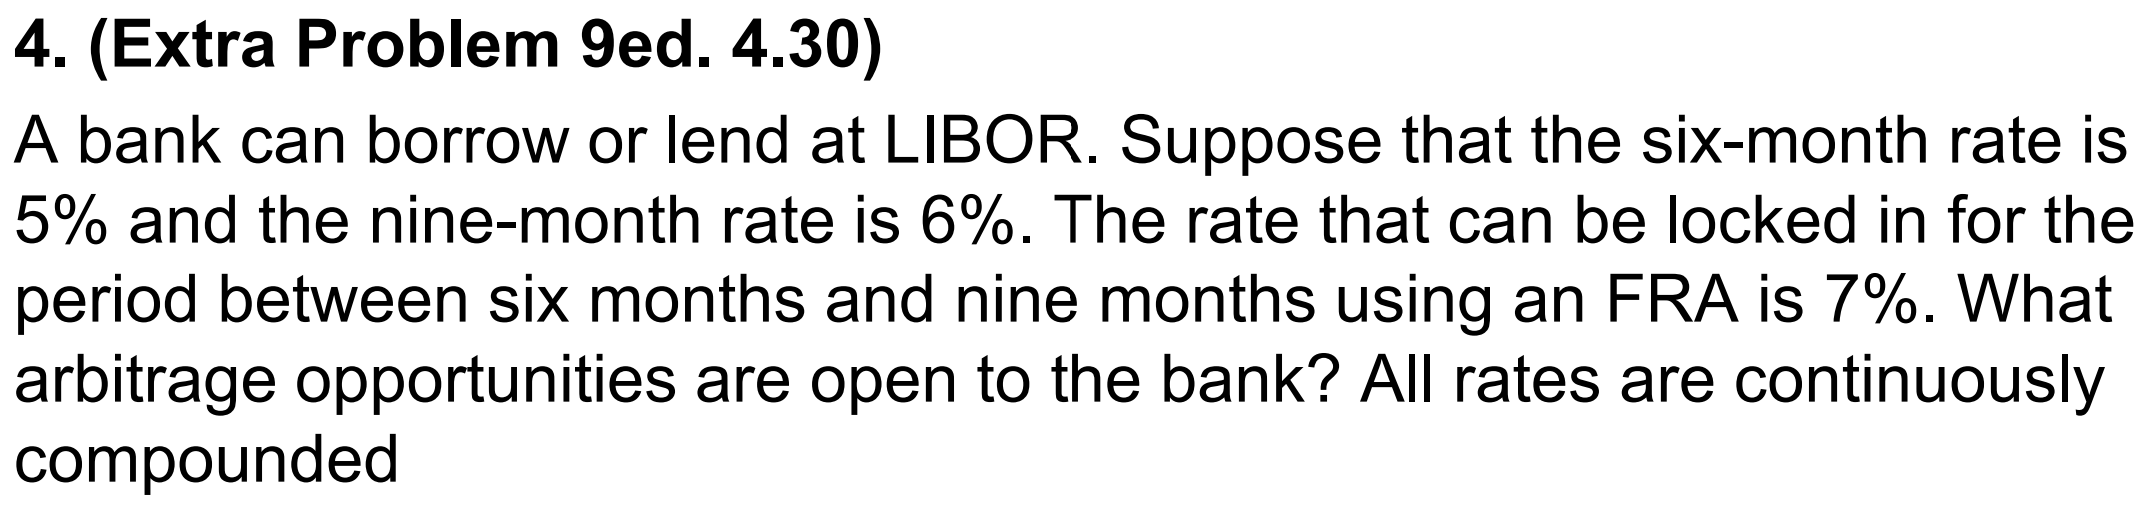
\includegraphics{images/선물옵션_4-30.png}

}

\caption{Chapter4-39, 9ed.}

\end{figure}%

\textbf{Solving}

먼저, 6개월 및 9개월 금리로부터 \(F_{6m,3m}\)의 균형가격을 산출하면,

\[F_{6m,3m}=\frac{\frac{9}{12}6\%-\frac{6}{12}5\%}{\frac{3}{12}}=8\%\]

그러나, 현재 FRA 계약금리는 7\%이므로 1\%p만큼 저평가되어있다.

따라서,

\begin{enumerate}
\def\labelenumi{\arabic{enumi}.}
\tightlist
\item
  6개월간 5\%로 자금을 빌리고
\item
  9개월간 6\%에 자금을 빌려주고,
\item
  FRA 매수계약(변동금리 수취 및 고정금리 지급)을 동일한 명목금액만큼
  체결 -\textgreater{} 6개월 후 9개월까지 3개월간 Libor금리로 자금을
  빌리면 FRA 계약금리인 7\%로 빌리는 효과
\end{enumerate}

9개월간 effective rate는
\(\frac{12}{9}(\frac{6}{12}5\%+\frac{3}{12}7\%)\approx 5.6667\%\)이므로,
\(0.333\%\)만큼 무위험 차익을 만들 수 있다.

\section*{Chapter5}\label{chapter5}
\addcontentsline{toc}{section}{Chapter5}

\markright{Chapter5}

\subsection*{\texorpdfstring{\textbf{Problem
5.1}}{Problem 5.1}}\label{problem-5.1}
\addcontentsline{toc}{subsection}{\textbf{Problem 5.1}}

\begin{figure}[H]

{\centering 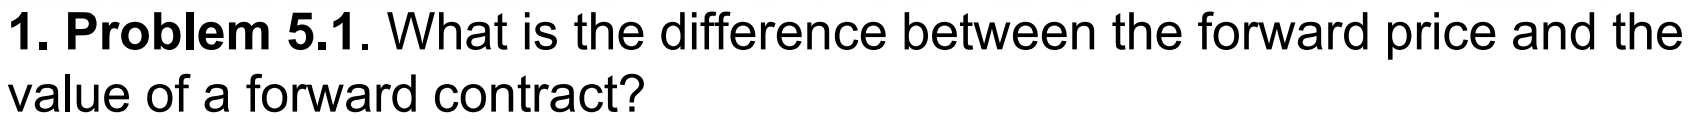
\includegraphics{images/선물옵션_5-1.png}

}

\caption{Chapter5-1}

\end{figure}%

Forward price : 선도가격

선도계약 체결시 계약당사자가 합의한 기초자산의 인도가격을 말하며,
기초자산의 현재가격과 선도계약 만기까지 기초자산을 보유하면서 발생하는
비용과 수익을 통해 이론적으로 산출할 수 있습니다.

Value of a forward contract : 선도계약의 가치

과거에 체결된 선도계약을 현재시점에서 평가할 때, 현재시점에서 동일한
선도계약을 체결한다면 예상되는 선도가격과 과거 체결시점의 선도가격의
차이로부터 산출되는 계약의 가치입니다. 즉, 과거의 선도계약을
현재시점에서 반대거래를 통해 청산하고자 할 때 예상되는 손익과 같습니다.

이를 통해, 현재시점에서 선도계약의 가치를 ``0''으로 만드는 가격이
이론적으로 산출되는 선도가격임을 알 수 있습니다.

\subsection*{\texorpdfstring{\textbf{Problem
5.7}}{Problem 5.7}}\label{problem-5.7}
\addcontentsline{toc}{subsection}{\textbf{Problem 5.7}}

\begin{figure}[H]

{\centering 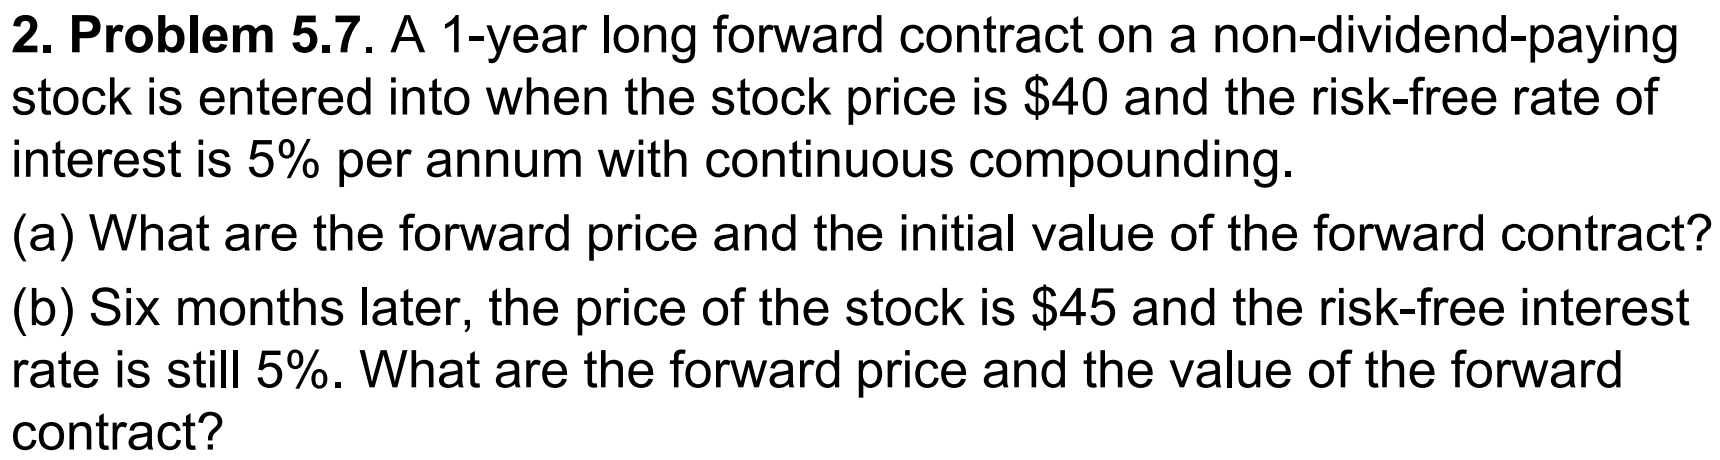
\includegraphics{images/선물옵션_5-7.png}

}

\caption{Chapter5-7}

\end{figure}%

\begin{enumerate}
\def\labelenumi{(\alph{enumi})}
\item
  선도가격 \(F=S_0e^{rT}=40e^{0.05}=42.05\), 현재시점의 선도계약의 가치
  ``0''
\item
  6개월 후의 선도가격 \(F=45e^{0.05\times 0.5}=46.14\), 이 때
  매수선도계약의 가치는 \(V_t-F_t=4.09\)
\end{enumerate}

\subsection*{\texorpdfstring{\textbf{Problem
5.10}}{Problem 5.10}}\label{problem-5.10}
\addcontentsline{toc}{subsection}{\textbf{Problem 5.10}}

\begin{figure}[H]

{\centering 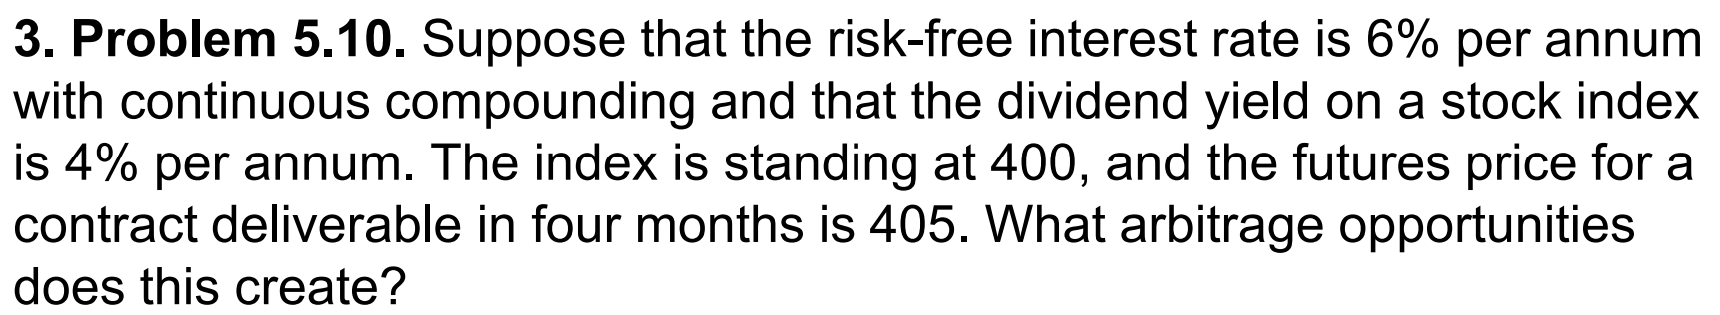
\includegraphics{images/선물옵션_5-10.png}

}

\caption{Chapter5-10}

\end{figure}%

무위험이자율 \(r_f=0.06\), 배당률 \(d=0.04\), 현재 지수가 \(400\)인
경우의 4개월 뒤 만기가 도래하는 주가지수선물의 이론가격은
\(F=400e^{\frac{4}{12}(0.06-0.04)}=402.68\)입니다.

그러나, 현재 주가지수선물의 시장가격은 405로 다소 고평가된 가격에
거래되고 있습니다. 따라서,

\begin{enumerate}
\def\labelenumi{(\arabic{enumi})}
\item
  현재시점에서 주가지수선물을 405에 매도하고
\item
  400만큼 무위험이자율에 자금을 차입하여,
\item
  해당 지수를 복제한 주식포트폴리오를 400에 매수한다면,
\end{enumerate}

4개월 뒤에 선물 만기도래시 주식포트폴리오를 405에 매도할 수 있고,
차입금에 대한 이자비용, 주식포트폴리오의 보유기간 동안 배당수익을 모두
합산하면 \(405-402.68=2.32\)만큼의 무위험 차익거래를 할 수 있습니다.

\subsection*{\texorpdfstring{\textbf{Problem
5.24}}{Problem 5.24}}\label{problem-5.24}
\addcontentsline{toc}{subsection}{\textbf{Problem 5.24}}

\begin{figure}[H]

{\centering 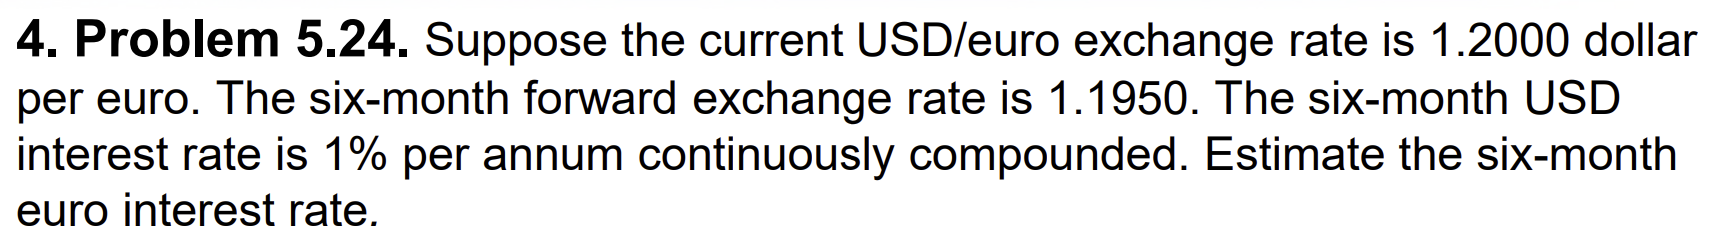
\includegraphics{images/선물옵션_5-24.png}

}

\caption{Chapter5-24}

\end{figure}%

\(S_0=1.2USD/EUR,\;F_0=1.195,\;r_{domestic}=0.01\)이면, 선도가격 수식을
통해 아래와 같이 산출가능합니다.

\[F_0=S_0e^{(r^d-r^f)T}\;\Rightarrow\;1.195=1.2e^{(0.01-r^f)0.5}\;\Rrightarrow\;r^f=0.0184\]

\section*{Chapter7 : Swap}\label{chapter7-swap}
\addcontentsline{toc}{section}{Chapter7 : Swap}

\markright{Chapter7 : Swap}

\subsection*{\texorpdfstring{\textbf{Problem
7.1}}{Problem 7.1}}\label{problem-7.1}
\addcontentsline{toc}{subsection}{\textbf{Problem 7.1}}

\begin{figure}[H]

{\centering 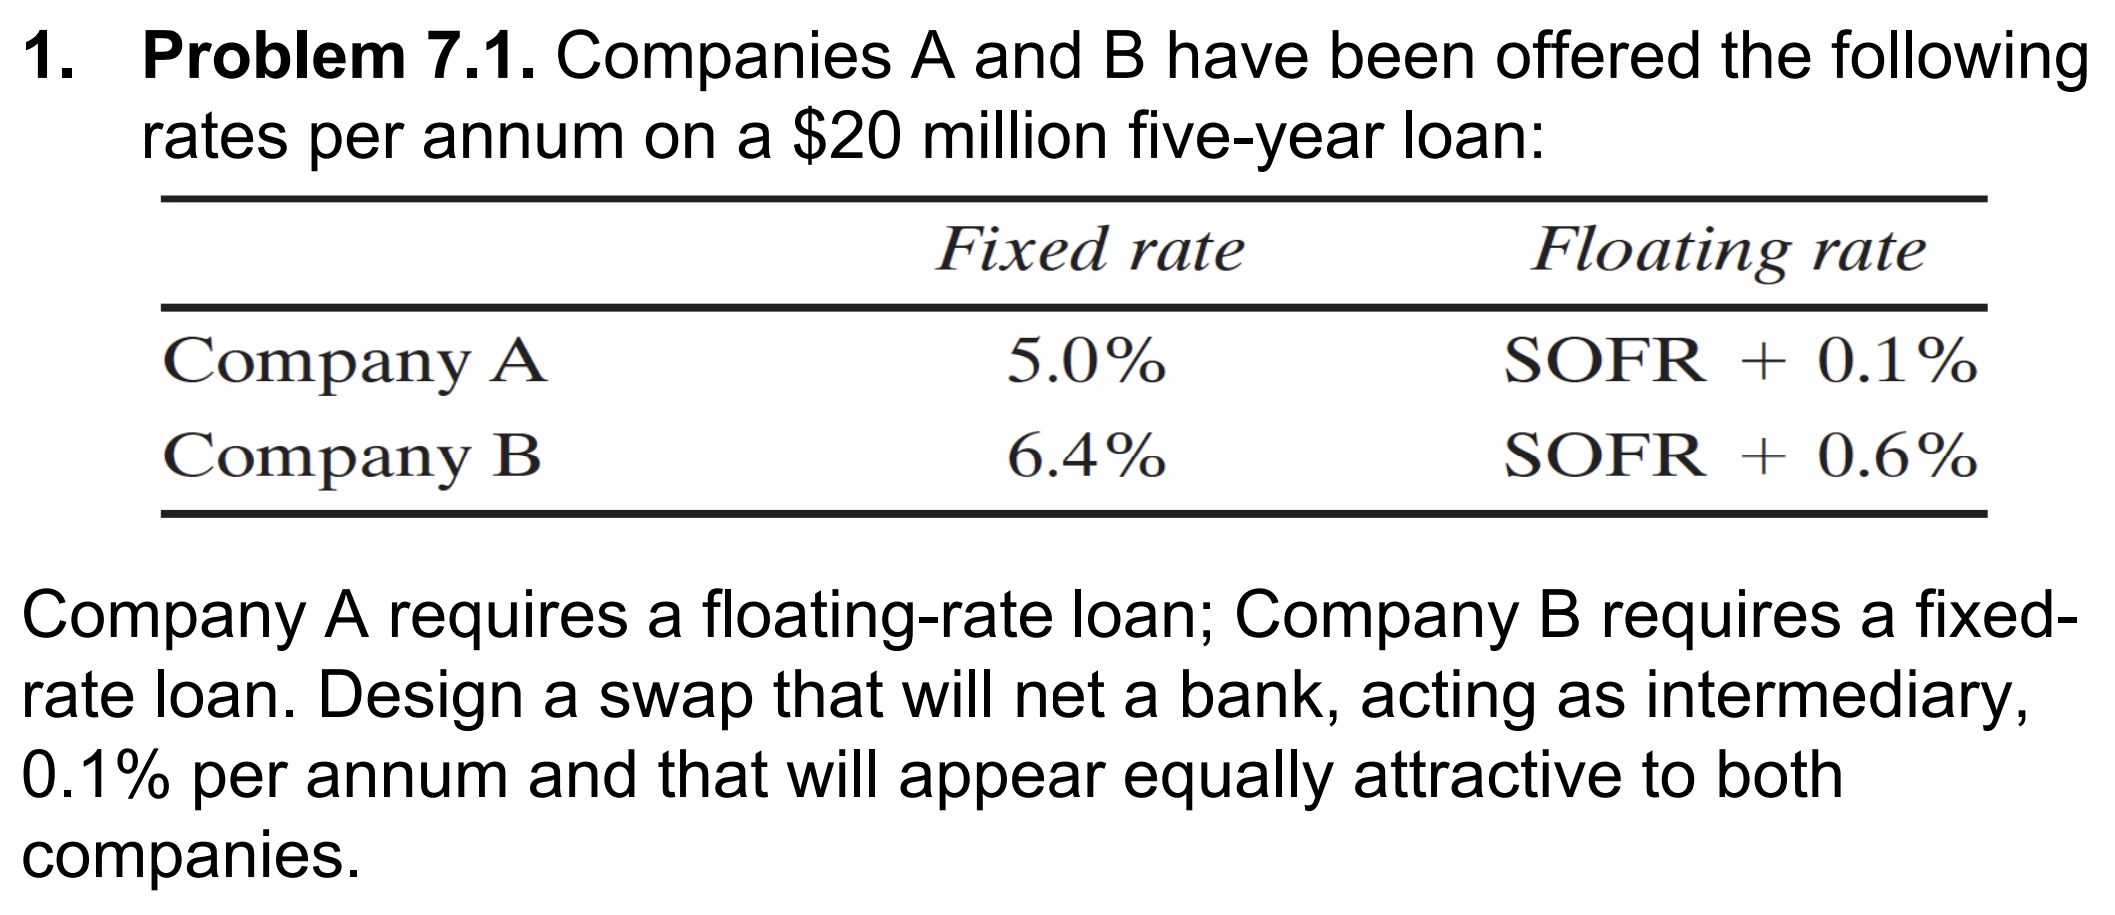
\includegraphics{images/선물옵션_7-1.png}

}

\caption{Chapter7-1}

\end{figure}%

두 회사를 비교하면 A는 Fixed rate에서 1.4\%만큼, Floating rate에서
0.5\%만큼 절대우위에 있습니다.

이를 다시이야기하면, A는 Fixed rate에서 비교우위가 있고 B는 Floating
rate에서 비교우위가 있다는 뜻과 같습니다.

A가 변동금리로 자금을 조달하고자 한다면 비교우위를 이용해서 고정금리로
먼저 돈을 빌리고, B와 스왑계약을 체결하면 됩니다.
(A=매도=고정금리수취,변동금리지급)

이 스왑계약이 SOFR와 Swap rate를 주고 받는 스왑이라면, A가 본인이 직접
변동금리로 조달하는 것보다 이익이 발생하는 swap rate는 4.9\%보다 크거나
같아야 합니다.

한편, B가 변동금리로 돈을 빌려서 스왑계약을 맺는 경우 B의 이익이
발생하는 swap rate는 5.8\% 보다 작거나 같아야합니다.

즉, Swap rate의 범위는 4.9\% \textasciitilde{} 5.8\%입니다. 여기서
은행이 양 회사를 중개하고 swap rate의 0.1\%를 수수료로 받는다면 Swap
rate는 5.0\% \textasciitilde{} 5.8\%에서 결정될 것 입니다.

예를 들어, Swap rate가 5.4\%에서 결정되는 경우,

A는 고정금리 5\%로 자금을 조달해서 SOFR를 지급하고 5.3\% 고정금리를
수취(0.1\%는 중개수수료)한다면 SOFR-0.3\%에 자금을 조달하는 효과로
0.4\%를 아낄 수 있고,

B는 변동금리 SOFR+0.6\%에 자금을 조달해서 5.4\%를 지급하고 SOFR를
수취한다면, 6.0\%에 자금을 조달하는 효과로, 0.4\%를 아낄 수 있습니다.

마지막으로, 비교우위간 차분인 0.9\%는 스왑을 이용한 비교우위전략으로
누릴 수 있는 총 효용으로 예시에서는 A가 0.4\%, B가 0.4\%, 중개기관이
0.1\%를 나눠서 누리게 됩니다.

\subsection*{\texorpdfstring{\textbf{Problem
7.4}}{Problem 7.4}}\label{problem-7.4}
\addcontentsline{toc}{subsection}{\textbf{Problem 7.4}}

\begin{figure}[H]

{\centering 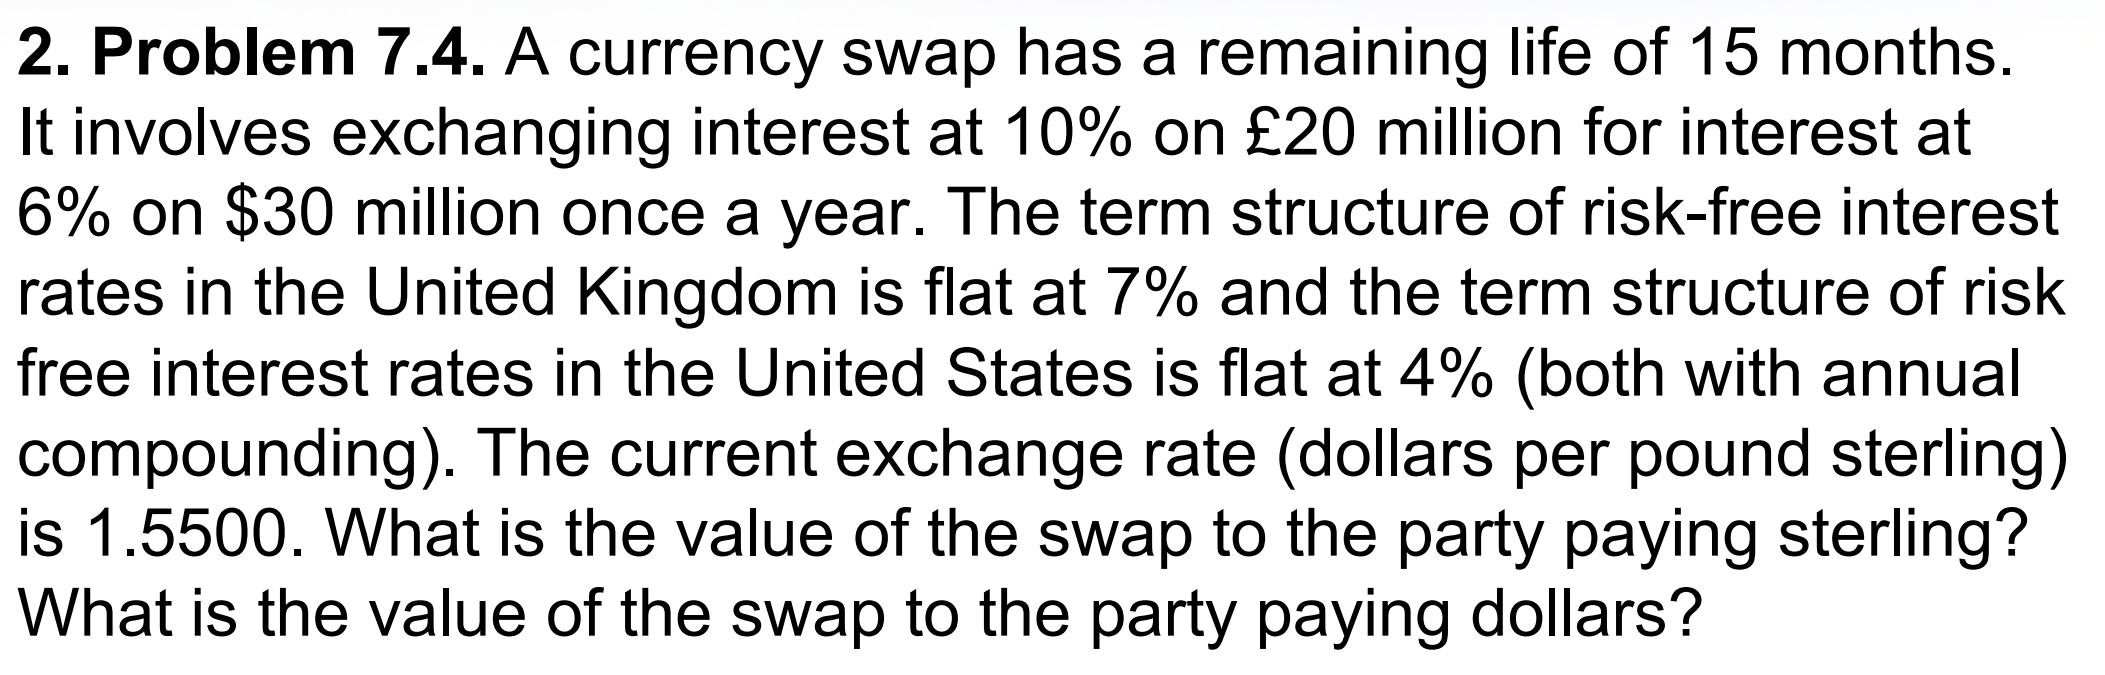
\includegraphics{images/선물옵션_7-4.png}

}

\caption{Chapter7-4}

\end{figure}%

해당 스왑계약은 Fixed-fixed currency swap이며, 현재 스왑계약의 잔존
현금흐름을 살펴보면, 3개월 뒤에 이자교환 + 9개월 뒤에 이자 교환 + 15개월
뒤에 원금과 이자 교환이 남았습니다.

미국을 자국, 영국을 타국으로 보면
\(S_0=1.55,\;r_f^d=0.04,\;r_f^f=0.07\)와 같고, 해당 스왑계약의 가치는
두가지 방법으로 평가할 수 있습니다.

\subsubsection*{(1) 선도환율을 이용한 현금흐름
방식}\label{uxc120uxb3c4uxd658uxc728uxc744-uxc774uxc6a9uxd55c-uxd604uxae08uxd750uxb984-uxbc29uxc2dd}
\addcontentsline{toc}{subsubsection}{(1) 선도환율을 이용한 현금흐름
방식}

먼저 3개월/9개월/15개월 뒤의 선도환율을 각각 계산해보겠습니다.

\[f_{3m}=1.55e^{ln\frac{1.04}{1.07}\times\frac{3}{12}},\;f_{9m}=1.55e^{ln\frac{1.04}{1.07}\times\frac{9}{12}},\;f_{15m}=1.55e^{ln\frac{1.04}{1.07}\times\frac{15}{12}}\]

\begin{tcolorbox}[enhanced jigsaw, toprule=.15mm, breakable, left=2mm, leftrule=.75mm, opacitybacktitle=0.6, coltitle=black, rightrule=.15mm, colback=white, titlerule=0mm, bottomtitle=1mm, colframe=quarto-callout-important-color-frame, title=\textcolor{quarto-callout-important-color}{\faExclamation}\hspace{0.5em}{Interest Compounding method}, toptitle=1mm, arc=.35mm, colbacktitle=quarto-callout-important-color!10!white, opacityback=0, bottomrule=.15mm]

문제의 이자율은 annual compounding이므로, 연속복리이자율을 사용해서
선도환율을 구하려면 continuous compounding으로 치환해서 이용해야 합니다.

즉,
\(1+r_{annual}=e^{r_{continuous}}\;\Rightarrow\;ln(1+r_{annual})=r_{continuous}\)

\end{tcolorbox}

이제, 기간별 sterling payer의 현금흐름을 살펴보면 아래와 같습니다.

\begin{longtable}[]{@{}crrcrc@{}}
\toprule\noalign{}
구분 & Cash-Inflow & Cash-Outflow & forward rate & Outflow(\$) & Net \\
\midrule\noalign{}
\endhead
\bottomrule\noalign{}
\endlastfoot
3month & \$1.8m & S2m & 1.54 & 3.08 & -1.278 \\
15month & \$31.8m & S22m & 1.50 & 32.91 & -1.109 \\
\end{longtable}

마지막으로, Net의 현재가치 -\$2.32m가 Sterling payer의 스왑계약 가치가
되며, Dollar payer의 가치는 정확히 반대가 됩니다.

\subsubsection*{(2) 채권 방식}\label{uxcc44uxad8c-uxbc29uxc2dd}
\addcontentsline{toc}{subsubsection}{(2) 채권 방식}

위의 현금흐름표를 보면, 각 통화의 현금흐름은 채권으로 환산하여 계산할 수
있습니다.

달러채권과 스털링채권의 현재공정가치를 각각 계산하면 아래와 같습니다.

\[Bond_{usd}=\frac{1.8}{(1+0.04)^{\frac{3}{12}}}+\frac{31.8}{(1+0.04)^{\frac{15}{12}}}\]

\[Bond_{sterling}=\frac{2}{(1+0.07)^{\frac{3}{12}}}+\frac{22}{(1+0.07)^{\frac{15}{12}}}\]

Sterling payer의 현금흐름은 달러채권을 사고 스털링채권을 발행하는 것과
동일하므로, 스왑의 가치는
\(B_{usd}-1.55\times B_{sterling}=32.061-1.55\times 22.182=-\$2.321m\)과
같습니다.

\subsection*{\texorpdfstring{\textbf{Problem
7.8}}{Problem 7.8}}\label{problem-7.8}
\addcontentsline{toc}{subsection}{\textbf{Problem 7.8}}

\begin{figure}[H]

{\centering 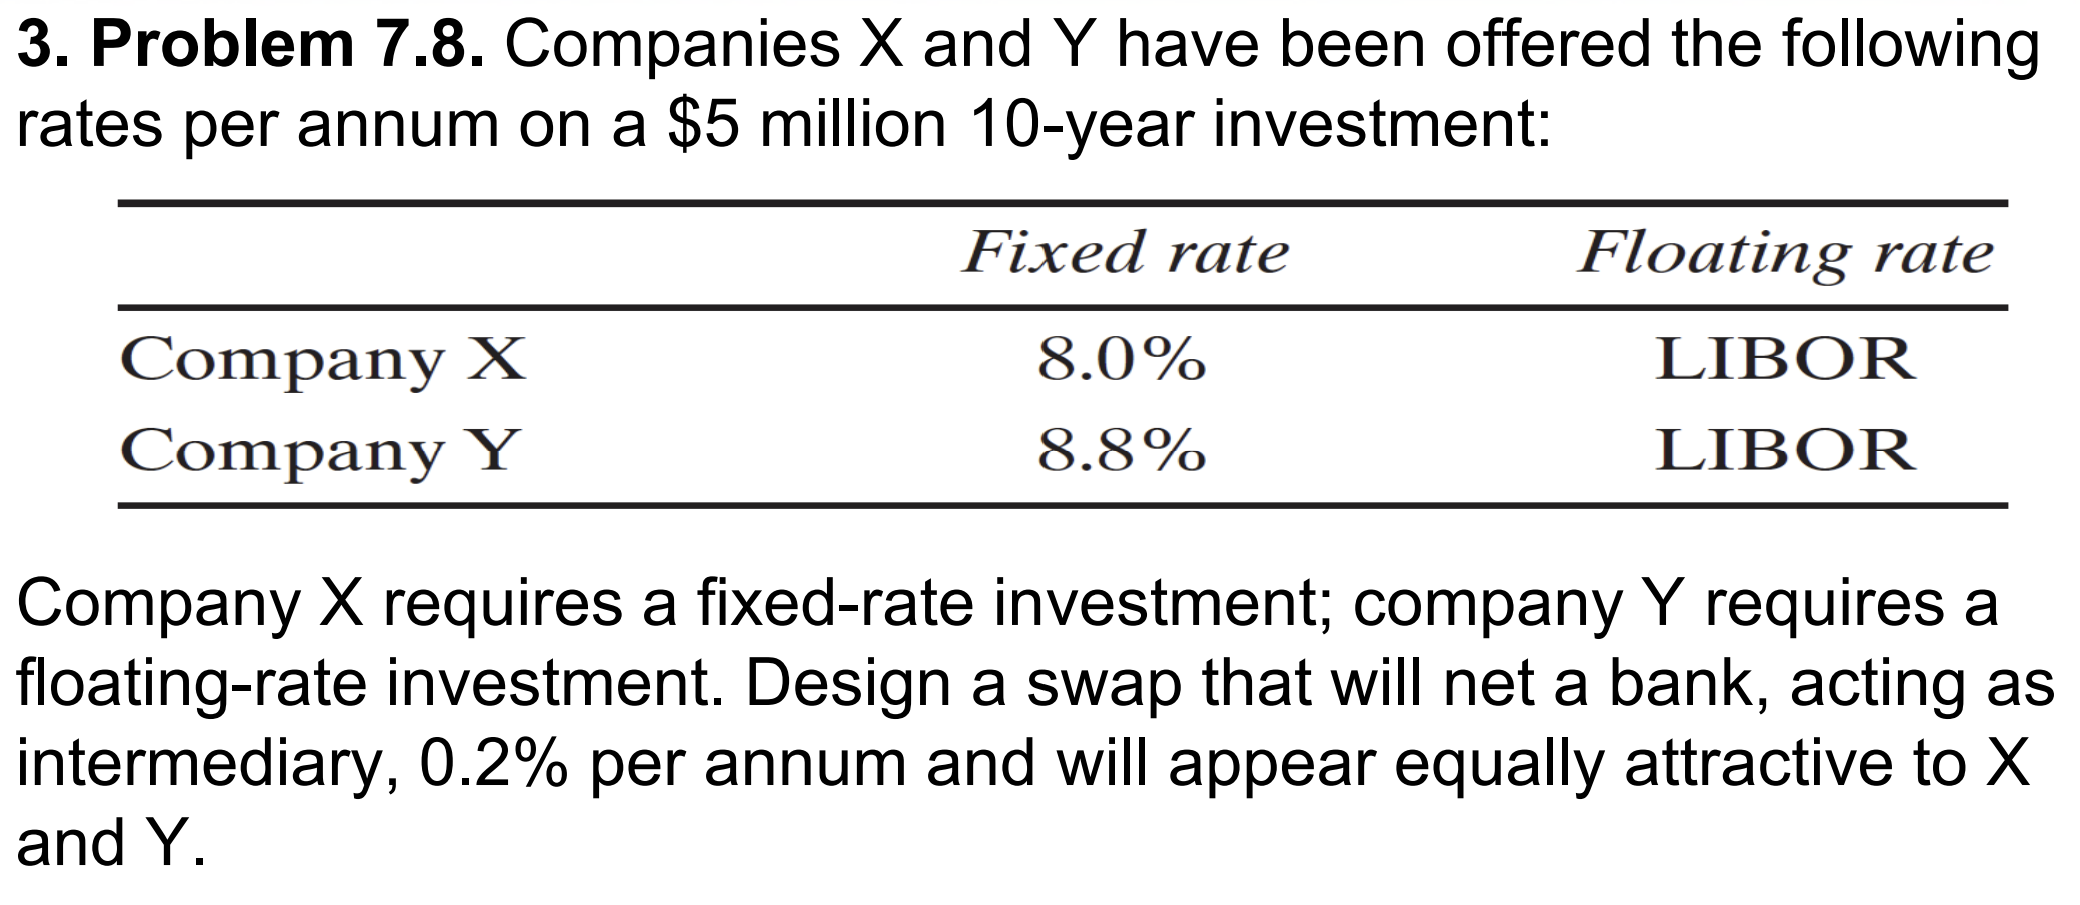
\includegraphics{images/선물옵션_7-8.png}

}

\caption{Chapter7-8}

\end{figure}%

Problem 7-1과 동일한 풀이방법입니다.

고정금리는 X가 0.8\%만큼 절대우위에 있고, 변동금리는 동일하므로 자금을
차입할 때의 비교우위는 X가 고정금리에, Y가 변동금리에 있습니다.

해당 상황은 투자이므로, 비교우위 활용은 X가 변동금리에 투자하고 Y와
스왑계약을 맺는 방법으로 이루어집니다.(X=매도=고정수취,변동지급)

스왑계약의 swap rate는 8\%\textasciitilde8.8\%에서 이루어질 수 있으며,
수수료 0.2\%를 감안하면 8.2\%\textasciitilde8.8\%에서 이루어질 것
입니다.

예를 들어, 8.5\%에서 이루어진다면

X는 Libor에 투자하고 (Libor지급-8.3\%수취) 스왑계약을 체결한다면 8.3\%인
고정금리에 투자하는 효과가 있어 0.3\%의 이익이 발생합니다.

마찬가지로 Y는 고정금리 8.8\%에 투자하고 (Libor수취-8.5\%지급)
스왑계약을 체결한다면 Libor+0.3\%에 투자하는 효과가 있어 0.3\%의 이익이
발생합니다.

총 효용인 0.8\%는 매수자(Y) 0.3\%, 매도자(X) 0.3\%, 중개인 0.2\%로
나누어 가집니다.

\subsection*{\texorpdfstring{\textbf{Problem
7.21}}{Problem 7.21}}\label{problem-7.21}
\addcontentsline{toc}{subsection}{\textbf{Problem 7.21}}

\begin{figure}[H]

{\centering 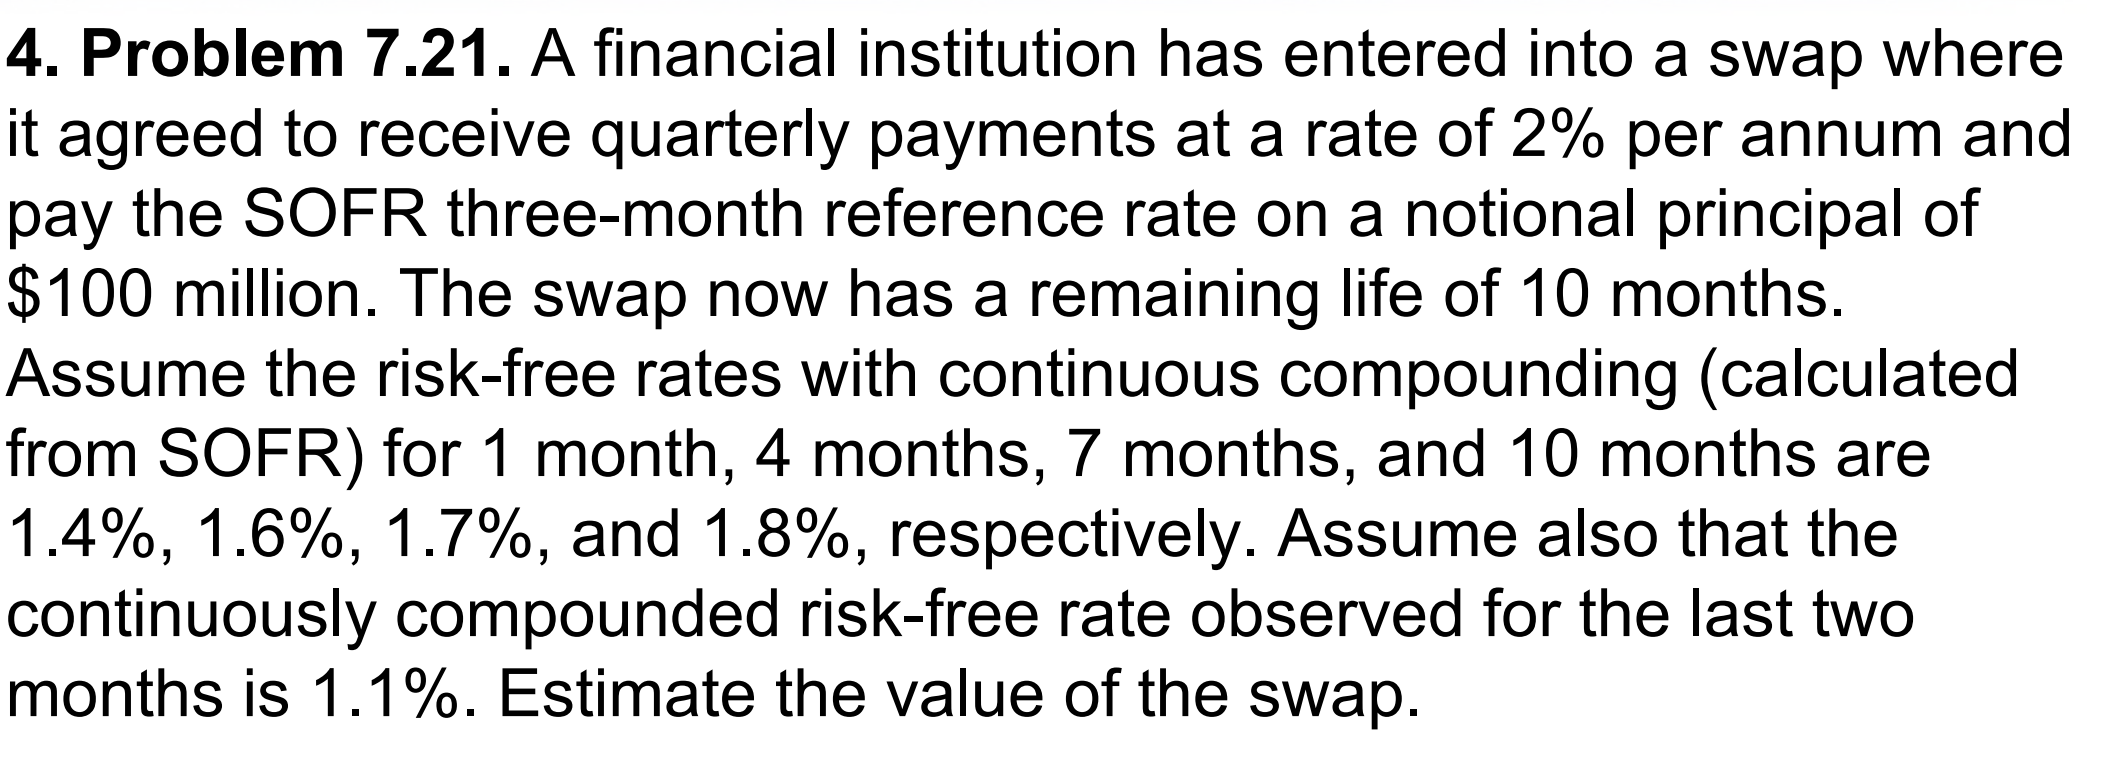
\includegraphics{images/선물옵션_7-21.png}

}

\caption{Chapter7-21}

\end{figure}%

해당 OIS는 OIS rate=2\% 및 SOFR를 3개월 주기로 명목금액 \$100m에 대해
교환하는 스왑계약입니다.

해당 스왑계약의 가치를 평가하기 위해서는 OIS를 SOFR를 지급하는 FRN과
2\%를 지급하는 채권으로 나누어서 각각 평가할 수 있습니다.

SOFR-FRN의 경우, 1개월 뒤 이자를 지급받은 직후에 가격이 Par value로
형성되어야 하는데 이를 이용해서 가치를 평가할 수 있습니다. 1개월 뒤
지급받을 이자는 \$0.3m이며 이자지급 직후 SOFR-FRN의 가격은 Par이므로,
현재가치는 \(100.3e^{-0.014\times\frac{1}{12}}=100.1831\)

2\% 지급 채권의 경우,
\(0.5\sum_{k=1}^4e^{-r_i\times\frac{3k-2}{12}}+100e^{-r_4\times\frac{10}{12}}=100.4956\)

해당 기관은 스왑매도(고정금리 수취, 변동금리 지급)이므로, FRN을 발행하고
2\% 채권을 매수한 것과 같습니다. 따라서 스왑계약의 가치는 아래와
같습니다.

\[Value_{OIS}=Bond_{2\%}-FRN=100.4956-100.1831=\$0.3124m\]

\begin{tcolorbox}[enhanced jigsaw, toprule=.15mm, breakable, left=2mm, leftrule=.75mm, opacitybacktitle=0.6, coltitle=black, rightrule=.15mm, colback=white, titlerule=0mm, bottomtitle=1mm, colframe=quarto-callout-note-color-frame, title=\textcolor{quarto-callout-note-color}{\faInfo}\hspace{0.5em}{OIS vs.~Libor-IRS}, toptitle=1mm, arc=.35mm, colbacktitle=quarto-callout-note-color!10!white, opacityback=0, bottomrule=.15mm]

Libor와 달리 Backward-looking 방식으로 산출되는 SOFR average rate를
이용하여 OIS를 체결하는 경우, 향후 변동금리는 현재시점에서 결정되지 않고
이자지급시점으로부터 과거 3개월간 SOFR를 누적하여 산출합니다.

즉, 10개월이 남은 현재 남은 이자지급시기는 1/4/7/10개월까지 4개인데,
1개월 뒤에 받게 될 변동금리는 과거 2개월 및 주어진 1개월간 SOFR 금리를
누적하여 산출됩니다.
\[e^{0.011\times\frac{2}{12}\times e^{0.014\times\frac{1}{12}}}\Rightarrow SOFR_{3month}=\frac{0.022+0.014}{3}=1.2\%\]

\end{tcolorbox}

\subsection*{\texorpdfstring{\textbf{Problem
7.22}}{Problem 7.22}}\label{problem-7.22}
\addcontentsline{toc}{subsection}{\textbf{Problem 7.22}}

\begin{figure}[H]

{\centering 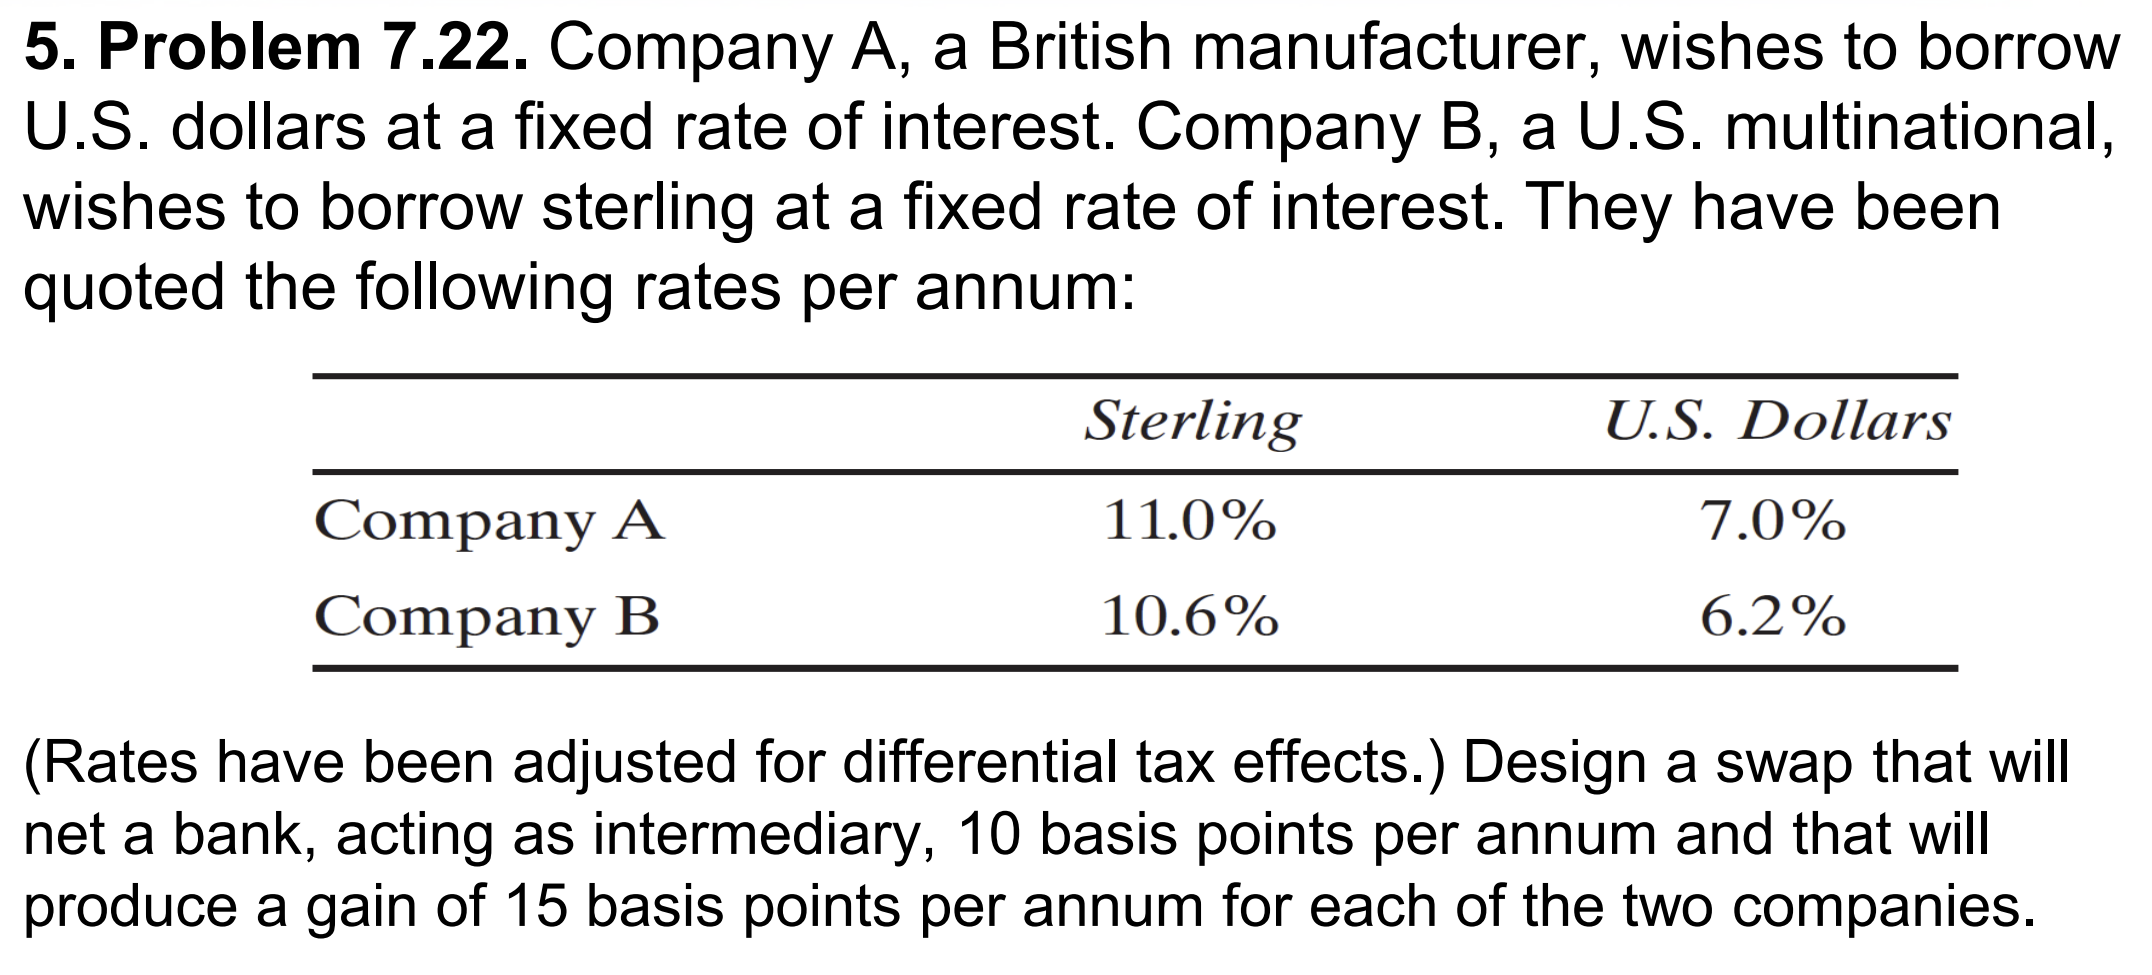
\includegraphics{images/선물옵션_7-22.png}

}

\caption{Chapter7-22}

\end{figure}%

Fixed-fixed Currency swap

A는 USD payer, USD 6.85\% pay / Sterling 11.0\% receive

B는 Sterling payer, Sterling 10.45\% pay / USD 6.2\% receive

And, 중개기관은 USD에서 0.65\% 이익 / Sterling에서 0.55\% 손실 - 0.1\%
차익 발생

\subsection*{\texorpdfstring{\textbf{Problem
7.extra1}}{Problem 7.extra1}}\label{problem-7.extra1}
\addcontentsline{toc}{subsection}{\textbf{Problem 7.extra1}}

\begin{figure}[H]

{\centering 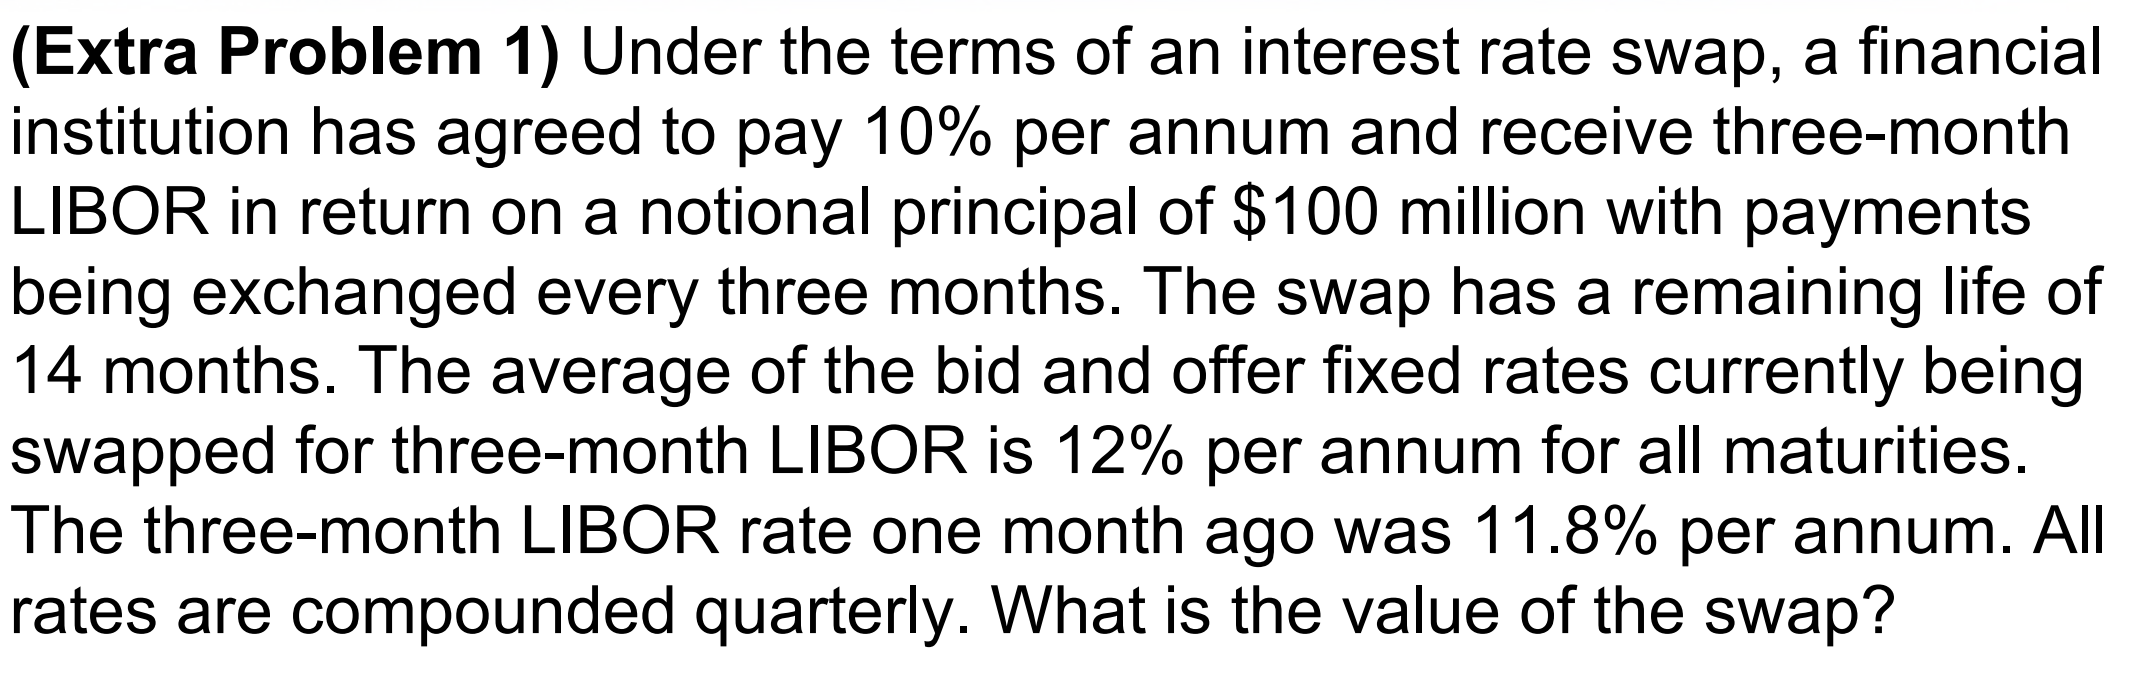
\includegraphics{images/선물옵션_7-extra1.png}

}

\caption{Chapter7-E1}

\end{figure}%

먼저, Libor-IRS의 구조를 Libor만큼 쿠폰을 지급하는 FRN과 Swap rate만큼
쿠폰을 지급하는 채권으로 구분한다면, 스왑계약 개시시점에서 FRN의 가치는
항상 Par value입니다.

개시시점에서 스왑계약의 가치는 0이므로, Swap rate만큼 쿠폰을 지급하는
채권의 가치도 par value가 되어야합니다. 즉, Swap rate는 스왑
개시시점에서 Par rate가 되므로, 이는 동일한 듀레이션을 가지는 채권의
YTM이 됩니다.

현재 bid-offer 중간값이 12\%라는 것은 swap rate가 모든 기간에 대해
12\%라는 뜻입니다. 즉, 채권의 yield curve가 12\%로 flat하다는
의미입니다. 이는 quarterly-compounding 금리로, 연속복리로 표현하면
\((1+0.12/4)^4=e^r\;\Rightarrow\;r=0.1182\)로 쓸 수 있습니다.

이제, 1개월 전 11.8\%에 체결된 스왑은 현재시점의 매수자(Swap rate지급,
Libor 수취) 입장에서 평가해보면, 14개월 남은 FRN과 11.8\% 쿠폰의 채권을
할인율 0.1182를 적용하여 비교하면 됩니다.

현재 FRN의 가치는 par value를 활용해 구할 수 있습니다. 2개월 후 쿠폰이
지급되고 난 직후 FRN의 가치는 par value가 될 것 입니다. 즉, 2개월 후
FRN의 가치는 100+2.95(쿠폰)입니다.

이를 현재가치로 환산하면 \(102.95e^{-0.1182\times\frac{2}{12}}=100.941\)

11.8\% 쿠폰의 채권의 현재가치는 아래와 같습니다.

\[2.5(e^{-0.1182\times\frac{2}{12}}+e^{-0.1182\times\frac{5}{12}}+e^{-0.1182\times\frac{8}{12}}+e^{-0.1182\times\frac{11}{12}})\]
\[+102.5e^{-0.1182\times\frac{14}{12}}=98.678\]

해당 기관은 Fixed rate payer이므로, FRN을 사고 11.8\% 쿠폰의 채권을
매도한 것과 같습니다. 즉, 스왑계약의 가치는
\(FRN-11.8\%\;Note=100.941-98.678=\$2.263m\)

\begin{tcolorbox}[enhanced jigsaw, toprule=.15mm, breakable, left=2mm, leftrule=.75mm, opacitybacktitle=0.6, coltitle=black, rightrule=.15mm, colback=white, titlerule=0mm, bottomtitle=1mm, colframe=quarto-callout-note-color-frame, title=\textcolor{quarto-callout-note-color}{\faInfo}\hspace{0.5em}{직관적인 풀이방법}, toptitle=1mm, arc=.35mm, colbacktitle=quarto-callout-note-color!10!white, opacityback=0, bottomrule=.15mm]

한편, Swap rate가 현재 12\%라는 것은 현재시점에서 동일한 스왑계약을
체결하면 고정금리가 12\%가 된다는 의미입니다.

즉, 1개월 전에 10\%를 지급하는 스왑계약을 현재시점에서 다시 체결한다면
12\%로 체결해야하므로, 2\%만큼 더 지급해야한다는 뜻입니다.

이러한 초과지급분을 모두 현재가치로 환산하면 현재 스왑의 가치가 될 것
입니다. 다만, 2개월 뒤 있을 최초 이자교환분은 이미 1개월 전에 11.8\%로
결정되었으므로 초과지급분은 1.8\%입니다.

\[0.45e^{-0.1182\times\frac{2}{12}}+0.5(e^{-0.1182\times\frac{5}{12}}+e^{-0.1182\times\frac{8}{12}}+e^{-0.1182\times\frac{11}{12}}+e^{-0.1182\times\frac{14}{12}})\]

\end{tcolorbox}

\subsection*{\texorpdfstring{\textbf{Problem
7.extra2}}{Problem 7.extra2}}\label{problem-7.extra2}
\addcontentsline{toc}{subsection}{\textbf{Problem 7.extra2}}

\begin{figure}[H]

{\centering 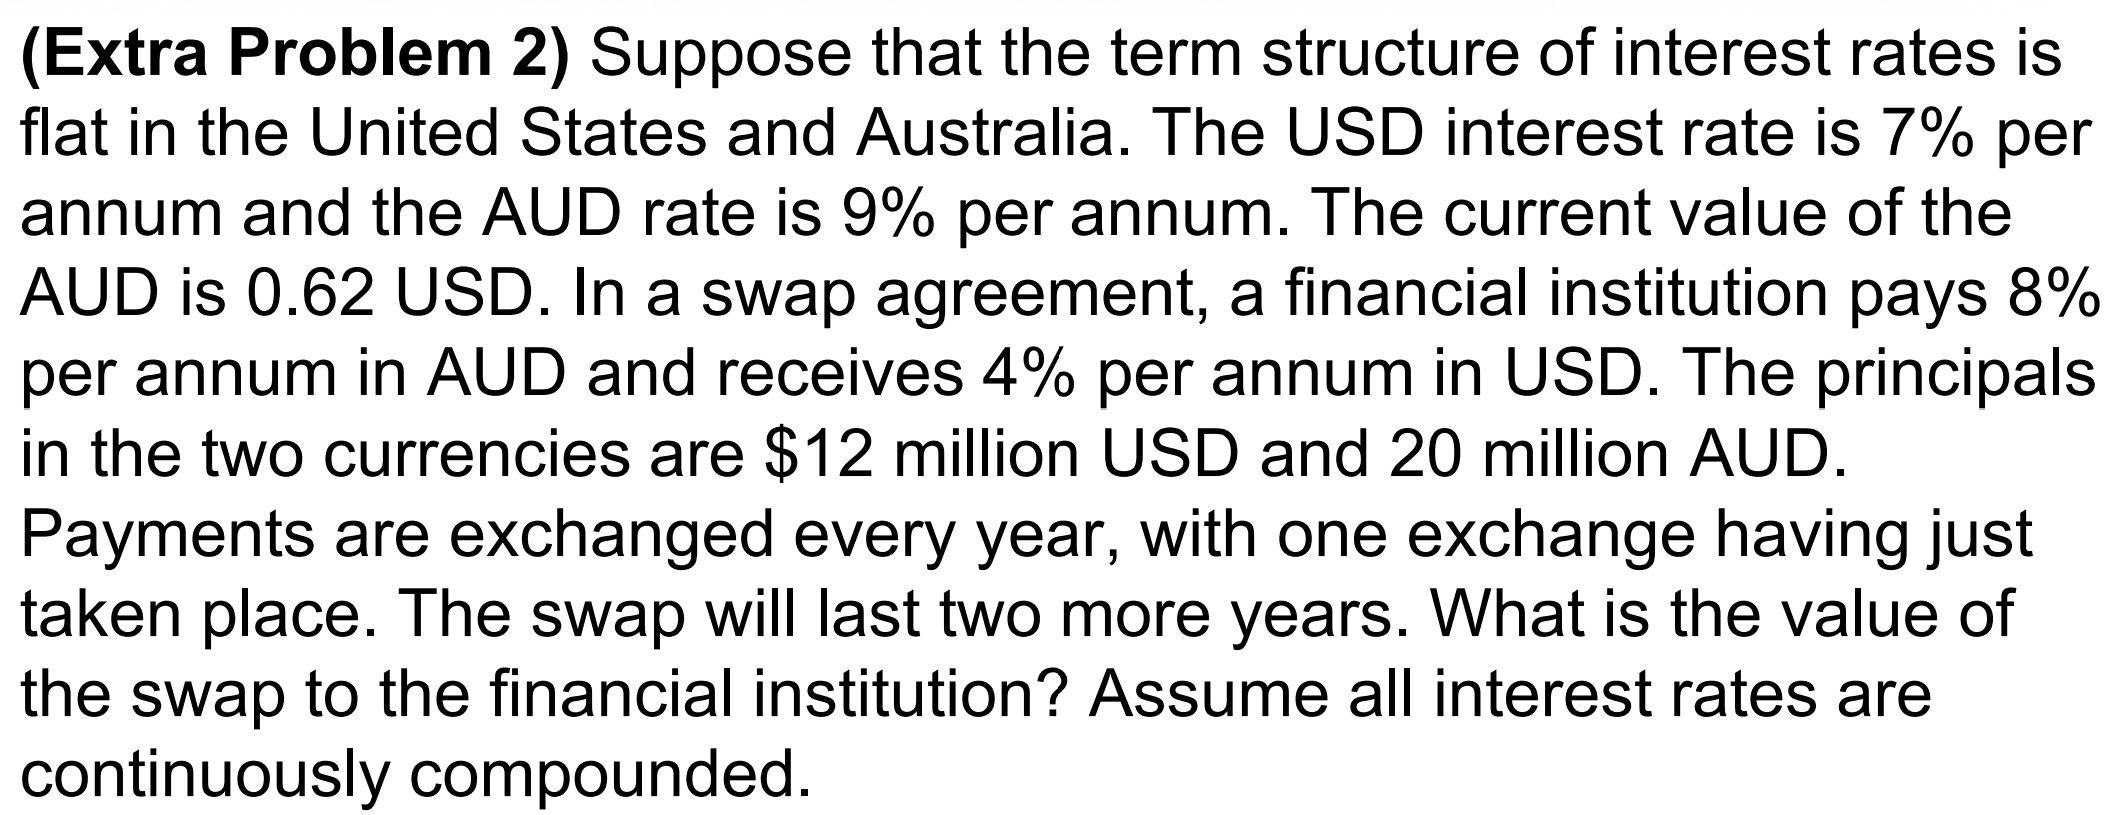
\includegraphics{images/선물옵션_7-extra2.png}

}

\caption{Chapter7-E2}

\end{figure}%

Continuous compounding 금리이므로, 선도환율을 이용하여 현금흐름을
할인하는 방식으로 스왑계약을 평가하겠습니다.

먼저, \(S_0=0.62,\;r_f^d=0.07,\;r_f^f=0.09\)이고 잔여 현금흐름은 1년뒤
이자교환 및 2년뒤 이자+원금교환입니다.

선도환율은 다음과 같습니다.

\[f_{1y}=0.62e^{0.07-0.09},\;f_{2y}=0.62e^{-0.02\times 2}\]

현금흐름을 정리하면 아래와 같습니다.

\begin{longtable}[]{@{}crrcrc@{}}
\toprule\noalign{}
구분 & Cash-Inflow & Cash-Outflow & forward rate & Outflow(\$) & Net \\
\midrule\noalign{}
\endhead
\bottomrule\noalign{}
\endlastfoot
1year & \$0.48m & AUD 1.6m & 0.608 & 0.972 & -0.492 \\
2year & \$12.48m & AUD 21.6m & 0.596 & 12.867 & -0.387 \\
\end{longtable}

달러로 표시된 Net의 현재가치 -\$0.795m가 스왑계약의 가치가 됩니다.

\section*{Chapter10 : Mechanics of Options
Markets}\label{chapter10-mechanics-of-options-markets}
\addcontentsline{toc}{section}{Chapter10 : Mechanics of Options Markets}

\markright{Chapter10 : Mechanics of Options Markets}

\subsection*{\texorpdfstring{\textbf{Problem 10.3,
10.13}}{Problem 10.3, 10.13}}\label{problem-10.3-10.13}
\addcontentsline{toc}{subsection}{\textbf{Problem 10.3, 10.13}}

\begin{figure}[H]

{\centering 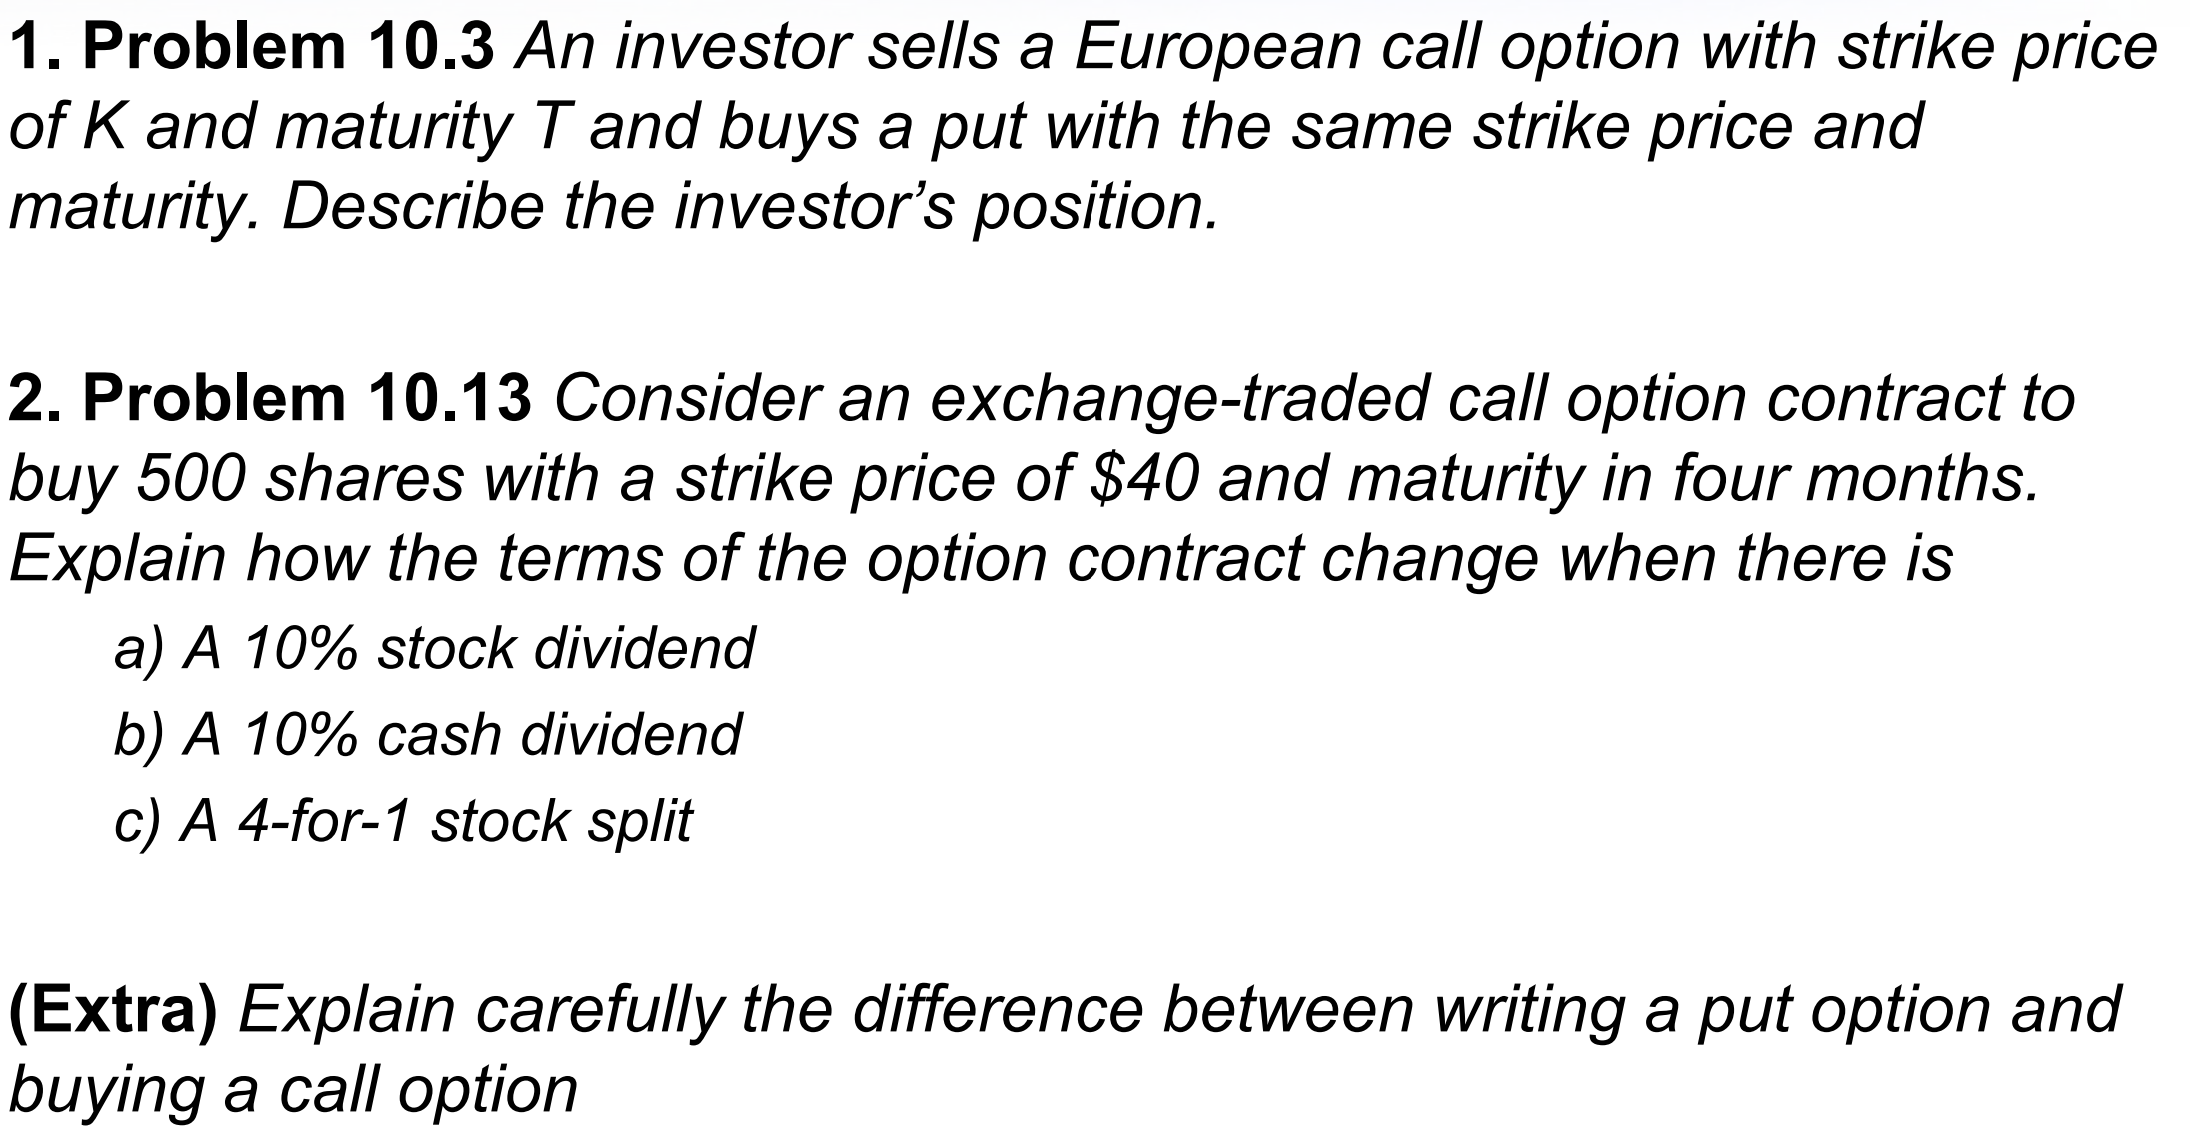
\includegraphics{images/선물옵션_10.png}

}

\caption{Chapter10}

\end{figure}%

\subsubsection*{\texorpdfstring{\textbf{10.3}}{10.3}}\label{section}
\addcontentsline{toc}{subsubsection}{\textbf{10.3}}

만기 T, 행사가격 K의 유럽형 콜옵션을 매도하고 풋옵션을 매수하는 경우
만기 Pay-off를 정리하면 아래와 같습니다.

\[-Max(S_T-K,0)+Max(K-S_T,0)=K-S_T\]

즉, 현재시점에서 액면 K의 무이표채에 투자하고 현물을 공매도하는 것과
동일한 포트폴리오입니다.

\begin{tcolorbox}[enhanced jigsaw, toprule=.15mm, breakable, left=2mm, leftrule=.75mm, opacitybacktitle=0.6, coltitle=black, rightrule=.15mm, colback=white, titlerule=0mm, bottomtitle=1mm, colframe=quarto-callout-tip-color-frame, title=\textcolor{quarto-callout-tip-color}{\faLightbulb}\hspace{0.5em}{Tip}, toptitle=1mm, arc=.35mm, colbacktitle=quarto-callout-tip-color!10!white, opacityback=0, bottomrule=.15mm]

Put-call parity :
\(c+Ke^{-rT}=p+S_0\Rightarrow p-c=Ke^{-rT}-S_0\)이므로, 위와 동일한
결과를 얻을 수 있습니다.

\end{tcolorbox}

\subsubsection*{\texorpdfstring{\textbf{10.13}}{10.13}}\label{section-1}
\addcontentsline{toc}{subsubsection}{\textbf{10.13}}

문제의 옵션은 만기는 4개월, 행사가격 40usd 및 거래승수 500에 대한 유럽형
콜옵션입니다.

\begin{enumerate}
\def\labelenumi{(\alph{enumi})}
\item
  만기 내 주식배당이 발생하는 경우, 행사가격 및 거래승수 변경을 통해
  옵션 보유자의 손익을 보전합니다. 10\%의 주식배당이 있으므로 콜옵션의
  행사가격은 \(40\times\frac{10}{11}\), 거래승수는
  \(500\times\frac{11}{10}\)으로 조정되고 손익에는 영향이 없습니다.
\item
  만기 내 10\%의 현금배당이 있는 경우, 별도의 옵션포지션 조정은 없으며
  배당락으로 주가가 10\%만큼 하락할 것 입니다. 따라서 콜옵션의 가치는
  하락합니다.
\item
  만기 내 4-for-1 주식분할이 발생하는 경우, 행사가격 및 거래승수 변경을
  통해 옵션 보유자의 손익을 보전합니다. 주식 보유자는 3주를 추가로
  받게되므로, 행사가격은 \(40/4=10\), 거래승수는 \(500*4=2000\)이
  됩니다. 손익에는 영향이 없습니다.
\end{enumerate}

\subsubsection*{\texorpdfstring{\textbf{Extra}}{Extra}}\label{extra}
\addcontentsline{toc}{subsubsection}{\textbf{Extra}}

콜매수와 풋매도는 모두 주가 상승시 포지션의 가치가 상승하는 구조입니다.
그러나 두 포지션은 근본적으로 권리를 가지고 있는지, 권리가 상대방에게
있어 계약이행의무만 있는지에 대한 차이가 있습니다.

콜옵션 매수 포지션은 권리를 가지고 있으며, 이에 따라 옵션 매수시
가격(프리미엄)을 매도자에게 지급하므로 초기비용이 발생합니다. 주식
가격이 상승하면 권리를 행사하여 이익을 실현할 것이고, 주식 가격이
행사가격보다 낮으면 권리를 포기함으로써 손실을 회피할 것 이므로 손실의
최대폭은 매수시 지불한 프리미엄으로 한정됩니다.

풋옵션 매도 포지션은 계약이행의무만 있으며, 이에 따라 옵션 매도시
프리미엄을 받게 되므로 초기수익이 발생합니다. 주식 가격이 상승하면
계약상대방은 권리행사를 포기하므로 프리미엄만큼 확정이익이 발생하고,
주식 가격이 행가가격보다 하락하면 계약상대방이 권리행사를 하게되므로,
손실이 발생합니다. 이익은 프리미엄으로 상한이 있으나 주가 상승에 따른
손실은 하방이 없습니다.

\section*{Chapter11 : Properties of Stock
Options}\label{chapter11-properties-of-stock-options}
\addcontentsline{toc}{section}{Chapter11 : Properties of Stock Options}

\markright{Chapter11 : Properties of Stock Options}

\subsection*{\texorpdfstring{\textbf{Problem 11.5, 18, 23, 24,
25}}{Problem 11.5, 18, 23, 24, 25}}\label{problem-11.5-18-23-24-25}
\addcontentsline{toc}{subsection}{\textbf{Problem 11.5, 18, 23, 24, 25}}

\begin{figure}[H]

{\centering 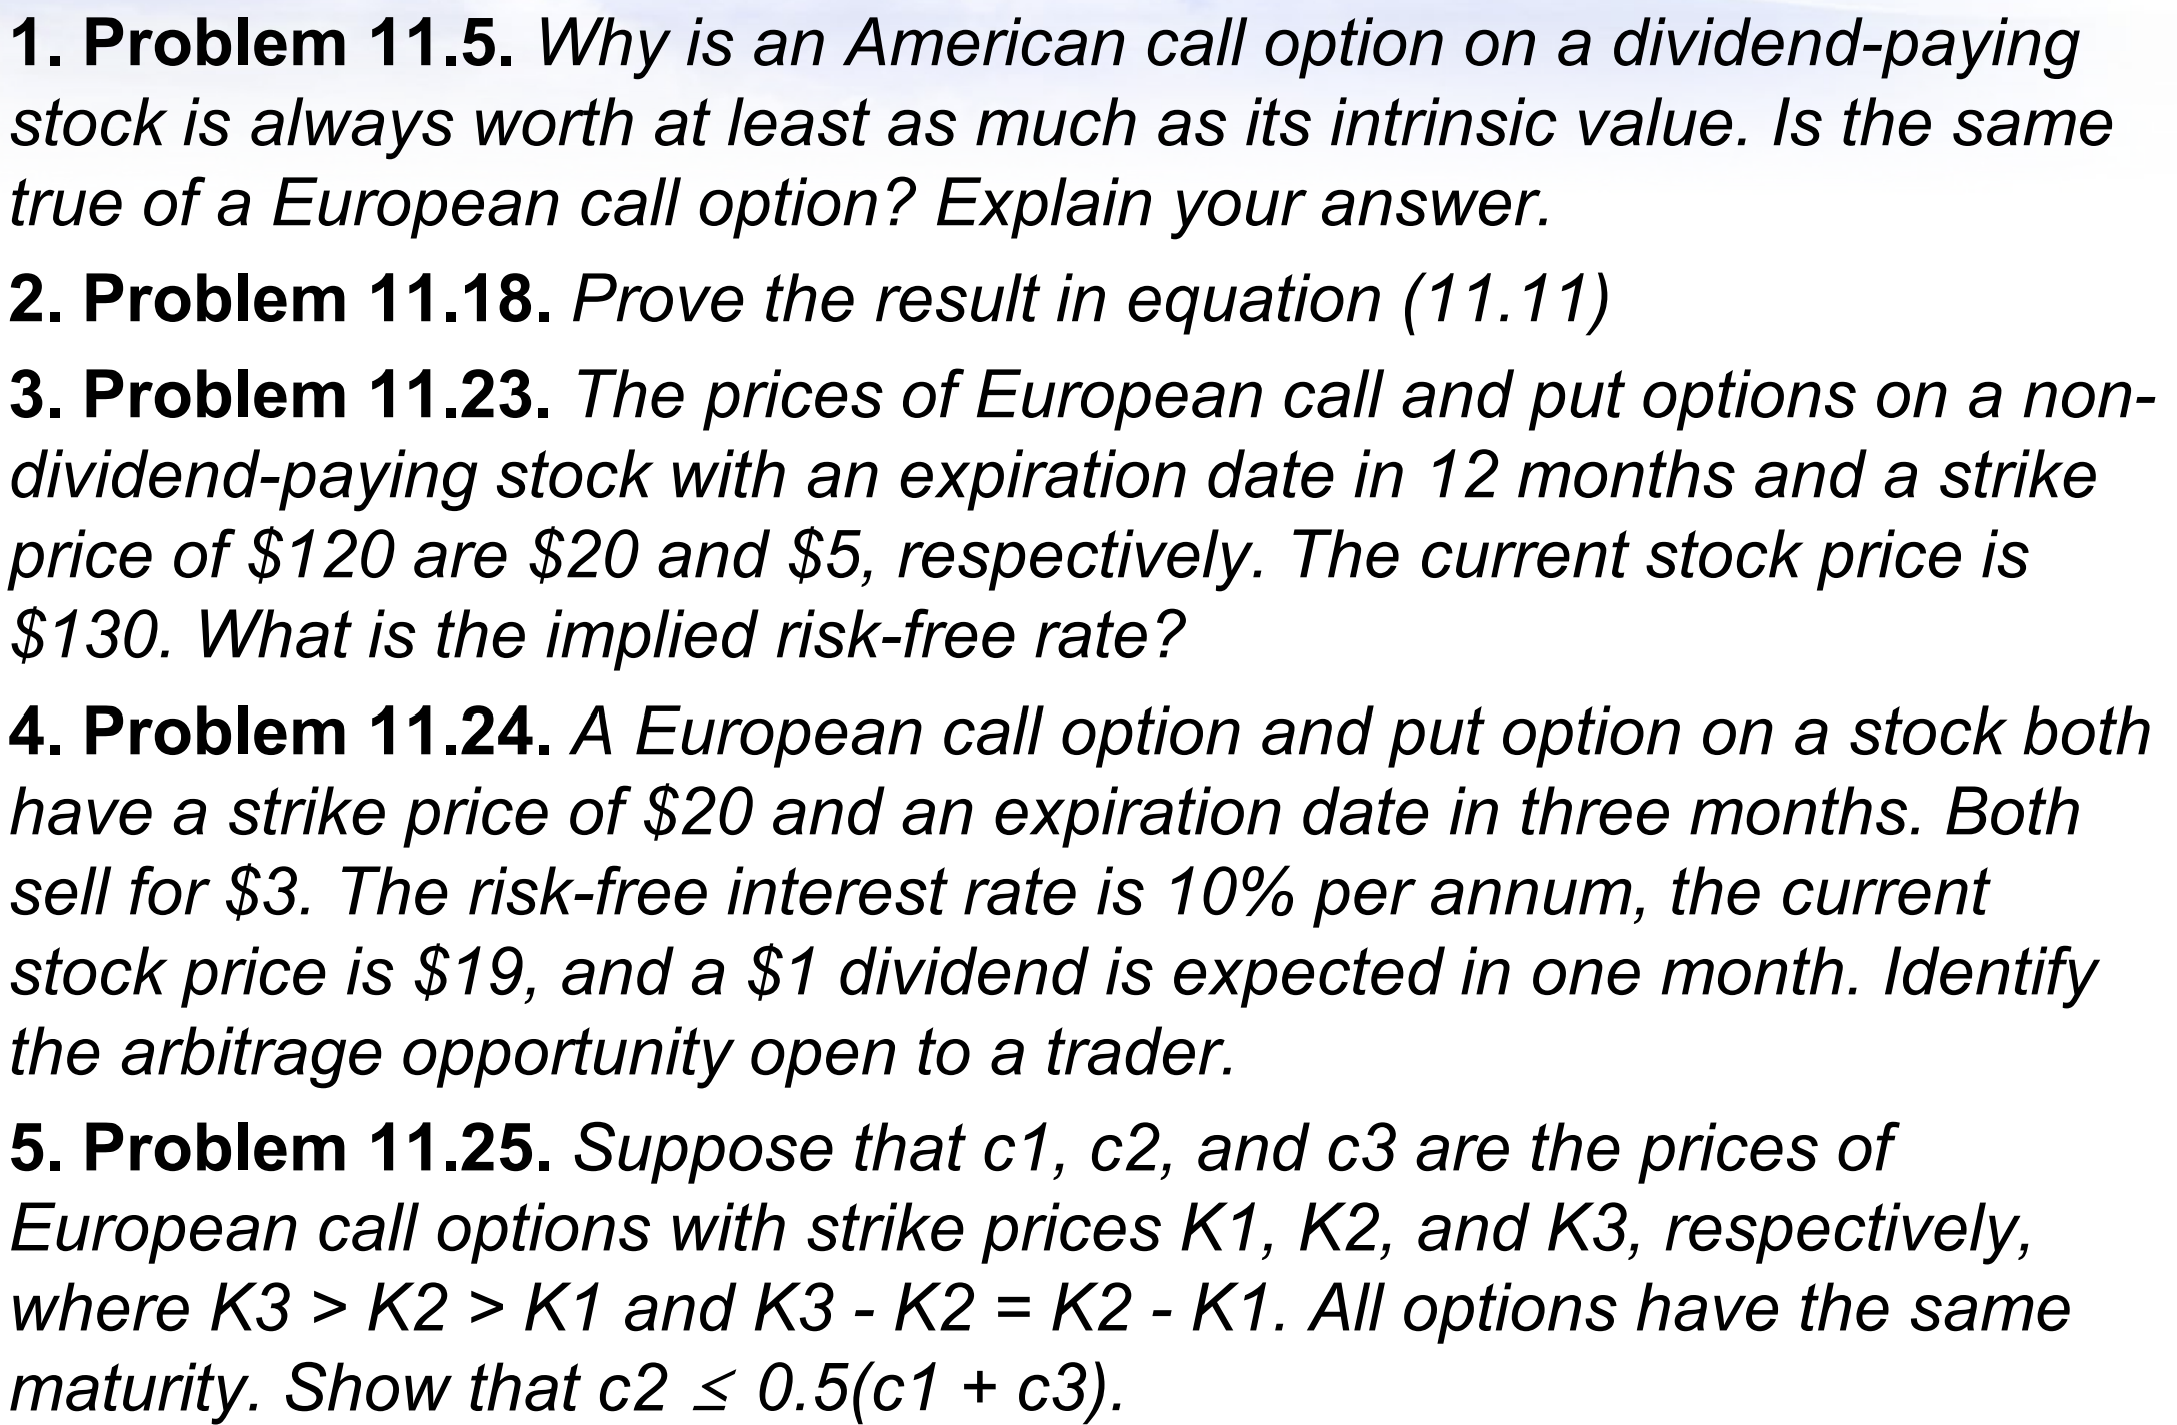
\includegraphics{images/선물옵션_11.png}

}

\caption{Chapter11}

\end{figure}%

\subsubsection*{\texorpdfstring{\textbf{11.5}}{11.5}}\label{section-2}
\addcontentsline{toc}{subsubsection}{\textbf{11.5}}

내재가치(intrinsic value)는 옵션을 현재시점에 권리행사한다면 얻을 수
있는 이익입니다. 따라서, 현재시점을 \(t\)라고 하면, 콜옵션의 내재가치는
\(max(S_t-K)\)입니다.

미국형 옵션은 옵션매수자가 원하는 때에 권리행사를 할 수 있으므로, 즉시
권리행사를 한다면 항상 내재가치만큼의 이익을 실현할 수 있습니다. 따라서
내재가치가 옵션가치의 하한이 됩니다.

한편, 유럽형 옵션은 만기시점에만 권리행사를 할 수 있으므로 기초자산에서
배당과 같은 중도현금흐름이 발생하면 옵션의 시간가치가 (-)로 형성될 수
있고, 이에 따라 내재가치보다 낮게 형성될 수 있습니다.

예를 들어, 다음달 배당이 예정된 주식에 대한 만기 2개월의 콜옵션을
보유하고 있다면 배당락이 발생하기 전에 권리행사를 통해 내재가치만큼
이익을 얻고, 배당수익도 누리는 것이 최적의 선택일 것입니다. 그러나,
유럽형 옵션은 만기까지 권리행사할 수 없으므로 이러한 콜옵션의 가격은
현재 내재가치보다 낮게 형성될 것 입니다.

\subsubsection*{\texorpdfstring{\textbf{11.18}}{11.18}}\label{section-3}
\addcontentsline{toc}{subsubsection}{\textbf{11.18}}

\textbf{?@sec-AmericanParity}

\subsubsection*{\texorpdfstring{\textbf{11.23}}{11.23}}\label{section-4}
\addcontentsline{toc}{subsubsection}{\textbf{11.23}}

각 파라미터는 \(T=1,\;S_0=130,\;K=120,\;c=20,\;p=5\)이므로, 풋콜패리티를
이용하면 다음과 같이 정리할 수 있습니다.

\[c+Ke^{-rT}=p+S_0\;\Rightarrow\;20+120e^{-r}=5+130 \Rightarrow r=\ln{\frac{120}{145}}\approx 4.26\%\]

\subsubsection*{\texorpdfstring{\textbf{11.24}}{11.24}}\label{section-5}
\addcontentsline{toc}{subsubsection}{\textbf{11.24}}

각 파라미터는
\(T=\frac{1}{4},\;K=20,\;r=0.1,\;S_0=19,\;D=1e^{-0.1/12},\;c=3,\;p=3\)입니다.

풋콜패리티를 이용하여 콜옵션의 가치를 평가해보면,

\[c+Ke^{-rT}+D=p+S_0\;\Rightarrow\;c+20e^{-0.025}+e^{-0.1/12}=3+19\;\Rightarrow\;c\approx 1.495\]

그러나, 현재 콜옵션의 시장가격이 3이므로 고평가되어있는 상태입니다.

따라서, (1) 콜옵션을 매도하고, 이와 동시에 (2) 풋옵션과 주식을 매수,
행사가격과 배당의 현재가치(\(Ke^{-rT}+D\))만큼의 무이표채권을
발행(자금을 차입)한다면, 현재시점에 1.505만큼 무위험차익을 얻을 수
있습니다.

\includegraphics[width=9.9in,height=1.44in]{Problems_files/figure-latex/mermaid-figure-1.png}

즉, 현재시점에 1.505만큼 수익이 발생하고 만기시점의 pay-off는 0이
됩니다.

\subsubsection*{\texorpdfstring{\textbf{11.25}}{11.25}}\label{section-6}
\addcontentsline{toc}{subsubsection}{\textbf{11.25}}

만기 Payoff를 살펴보면 확인 가능합니다.



\end{document}
